%!TEX TS-program = pdflatex
% dissertation.tex -- main dissertation file
%
% Wisconsin dissertation template
% Copyright (c) 2008-2009 William C. Benton.  All rights reserved.
%
% This program can redistributed and/or modified under the terms
% of the LaTeX Project Public License Distributed from CTAN
% archives in directory macros/latex/base/lppl.txt; either
% version 1 of the License, or (at your option) any later version.
%
% This program includes other software that is licensed under the
% terms of the LPPL and the Perl Artistic License; see README for details.
%
% You, the user, still hold the copyright to any document you produce
% with this software (like your dissertation).
%

%%% You'll want ``oneside'' for the deposit version, but probably not for any versions that don't need to meet the UW requirements
\documentclass[12pt,oneside,letterpaper]{memoir}
\setulmarginsandblock{3cm}{3cm}{*}
\setlrmarginsandblock{3cm}{3cm}{*}
\checkandfixthelayout

% why does this need to be here
\usepackage[usenames]{color}
\usepackage{mdframed}
\usepackage{framed}

%\usepackage{todonotes}
% compile without to do notes:
\usepackage[disable]{todonotes}

% preamble.tex -- packages to include
%
% Wisconsin dissertation template
% Copyright (c) 2008 William C. Benton.  All rights reserved.
%
% This program can redistributed and/or modified under the terms
% of the LaTeX Project Public License Distributed from CTAN
% archives in directory macros/latex/base/lppl.txt; either
% version 1 of the License, or (at your option) any later version.
%
% This program includes other software that is licensed under the
% terms of the LPPL and the Perl Artistic License; see README for details.
%
% You, the user, still hold the copyright to any document you produce
% with this software (like your dissertation).

%% You should use natbib
\IfFileExists{natbib.sty}{%
\usepackage{natbib}%
}{}

%% You probably need appendix, if you want appendices
\IfFileExists{appendix.sty}{%
\usepackage{appendix}%
}{}

%% the spacing in memoir is weird, you'll need to use this
\DisemulatePackage{setspace}
\usepackage[onehalfspacing]{setspace}

%% List setup; the ``hanglist`` environment will allow you to have
%% nicely-typeset enumerated lists (i.e. with the numbers hanging in
%% the margins).  You need at least version 2.1 of enumitem.sty.  If
%% you don't have enumitem installed at all, hanglist will just be an
%% alias for enumerate.
\IfFileExists{enumitem.sty}{%
\usepackage[loadonly]{enumitem}[2007/06/30]%
\newlist{hanglist}{enumerate}{1}% 
\setlist[hanglist]{label=\arabic*.}%
\setlist[hanglist,1]{leftmargin=0pt}%
}{%
\newenvironment{hanglist}{\begin{enumerate}}{\end{enumerate}}%
}

%% Comment out any of these that you don't want
\usepackage{amssymb}
\usepackage{amsmath}
\usepackage{amsthm}
%\usepackage{theorem}
\usepackage{hyperref}

\IfFileExists{mathpartir.sty}{%
\usepackage{mathpartir}%
}{}

%%%%% LISTINGS package and setup
\IfFileExists{listings.sty}{%
\usepackage{listings}%
}{}



%% Get rid of ugly borders around PDF hyperlinks (e.g. for cross-references, bib entries, or URLs)
\hypersetup{pdfborder = 0 0 0}

%% You want microtype.
\IfFileExists{microtype.sty}{%
\usepackage[protrusion=true,expansion=true]{microtype}%
}{}

%\pagestyle{thesisdraft}

% Surround parts of graphics with box
\usepackage{boxedminipage}

%% booktabs (thx to Nate Rosenblum for bringing this beautiful package
%% to my attention)
\IfFileExists{booktabs.sty}{%
\usepackage{booktabs}%
}{}

% This is now the recommended way for checking for PDFLaTeX:
\usepackage{ifpdf}

%% Avoid ugly "Type 3" fonts
\usepackage{lmodern}
\usepackage[LY1]{fontenc}

%% Substitute your favorite serif and sans fonts here....
\IfFileExists{tgpagella.sty}{%
% TeX Gyre pagella, like Palatino
\usepackage{tgpagella}%
}{}

\usepackage[LY1]{eulervm}

\ifpdf
\usepackage[pdftex]{graphicx}
\else
\usepackage{graphicx}
\fi

\usepackage{makeidx}
\makeindex

{\theoremstyle{plain}
\newtheorem{thm}{Theorem}[chapter]
\newtheorem{cor}[thm]{Corollary}
\newtheorem{define}[thm]{Definition}
\newtheorem{exmpl}[thm]{Example}
}
{\theoremstyle{remark}
\newtheorem{rmk}[thm]{Remark}
}

\newtheoremstyle{customsty1}
{3pt}%
{3pt}%
{}% --- body font
{}% --- indent amount
{\bfseries}% --- Theorem head font
{:}% --- Punctuation after head
{.5em}% --- space after head
{}% --- theorem head spec (can be left empty, meaning 'normal')

% Define 'newtheorems' that use ``customsty1''
{\theoremstyle{customsty1} 
}


%%% NB: the ``deposit'' chapter- and page- styles should conform to UW
%%% requirements.  If you are producing a pretty version of your
%%% dissertation for web use later, you will certainly want to make
%%% your own chapter and page styles.

\makechapterstyle{deposit}{%
  \renewcommand{\chapterheadstart}{}
  \renewcommand{\printchaptername}{}
  \renewcommand{\chapternamenum}{}
  \renewcommand{\printchapternum}{\parbox{2em}{\MakeLowercase{\Large\scshape\thechapter{}}} }
  \renewcommand{\afterchapternum}{}
  \renewcommand{\printchaptertitle}[1]{%
  \raggedright\Large\scshape\MakeLowercase{##1}}
  \renewcommand{\afterchaptertitle}{%
  \vskip\onelineskip \hrule\vskip\onelineskip}
}

\makepagestyle{deposit}
 
\makeatletter
 
\renewcommand{\chaptermark}[1]{\markboth{#1}{}}
\renewcommand{\sectionmark}[1]{\markboth{#1}{}}
 
\makeevenfoot{deposit}{}{}{}
\makeoddfoot{deposit}{}{}{}
\makeevenhead{deposit}{\thepage}{}{}
\makeoddhead{deposit}{}{}{\thepage}
\makeatother

%%% set up page numbering for chapter pages to satisfy UW requirements
%%% NB: You will want to delete until the ``SNIP'' mark if you are
%%% making a ``nice'' copy
\copypagestyle{chapter}{plain}
\makeoddfoot{chapter}{}{}{}
\makeevenhead{chapter}{\thepage}{}{}
\makeoddhead{chapter}{}{}{\thepage}
%%% SNIP

%%% bib nonsense
\makeatletter
\newenvironment{wb-bib}[1]{%
  \chapter*{references}
\ifnobibintoc\else 
\phantomsection 
\addcontentsline{toc}{chapter}{References} 
\fi 
\prebibhook
  \begin{bibitemlist}{#1}}{\end{bibitemlist}\postbibhook}

\AtBeginDocument{%
  \@ifpackageloaded{natbib}{% natbib is loaded
    \addtodef{\endthebibliography}{}{\vskip-\lastskip\postbibhook}
    \@ifpackagewith{natbib}{sectionbib}{% with sectionbib option
      \renewcommand{\bibsection}{\@memb@bsec}}%
      {\renewcommand{\bibsection}{\@memb@bchap}}}%
  {}
  \@ifpackagewith{chapterbib}{sectionbib}{%
    \renewcommand{\sectionbib}[2]{}
    \renewcommand{\bibsection}{\@memb@bsec}}{}
}
\makeatother

% defs.tex -- wbepi environment for chapter epigraphs and other useful defs.
%
% Wisconsin dissertation template
% Copyright (c) 2008 William C. Benton.  All rights reserved.
%
% This program can redistributed and/or modified under the terms
% of the LaTeX Project Public License Distributed from CTAN
% archives in directory macros/latex/base/lppl.txt; either
% version 1 of the License, or (at your option) any later version.
%
% This program includes other software that is licensed under the
% terms of the LPPL and the Perl Artistic License; see README for details.
%
% You, the user, still hold the copyright to any document you produce
% with this software (like your dissertation).


%% put lstnewenvironment declarations here, if you're using listings

%% end lstnewenvironment declarations

%% I put convenience definitions that will go in several chapters here

%%%%% begin convenience definitions

\makeatletter
\newcommand{\wb@episource}{}
\newenvironment{wbepi}[1]{\begin{quote}\renewcommand{\wb@episource}{#1}\itshape}{\par\upshape \raggedleft --- \textsc{\wb@episource}\\ \end{quote}}
\makeatother

%%%%% SVN
\IfFileExists{svn-multi.sty}{%
\usepackage{svn-multi}%
%%% Uncomment the second one and comment out the first one if you want
%%% to include subversion revision information in each file.
\newcommand{\vcinfo}{}%
%\newcommand{\vcinfo}{\begin{centering}\fbox{\fbox{\parbox{5in}{Author: \svnauthor\\Revision: \svnfilerev\\Last changed on: \svnfiledate\\URL: \svnkw{HeadURL}}}}\\[1em]\end{centering}}%
}{%
\newcommand{\svnidlong}[4]{}%
\newcommand{\svnfilerev}{}%
\newcommand{\svnauthor}{}%
\newcommand{\svnfiledate}{}%
\newcommand{\svnkw}{}%
\newcommand{\vcinfo}{}%
}

%%%%% end convenience definitions

% thesisdefs.tex

% This is mostly adapted from withesis.cls.  The original copyright
% notice for withesis.cls follows, preceded by two percent signs (%%):

%% withesis.cls
%% LaTeX Style file for the University of Wisconsin-Madison Thesis Format
%% Adapted from the Purdue University Thesis Format
%% Originally by Dave Kraynie
%% Edits by Darrell McCauley
%% Adapted to UW-Madison format by Eric Benedict  (Noted with <EB>)
%% Updated to LaTeX2e by Eric Benedict 24 July 00
%% 
%%=============================================================================
%% Licensed under the Perl Artistic License.
%% see: http://www.ctan.org/tex-archive/help/Catalogue/licenses.artistic.html
%% for more info...
%%=============================================================================

% withesis.cls is available from CTAN.  The modifications to this file
% are also licensed under the Perl Artistic License.

% --wb, 2008

\makeatletter

\newcounter {tocpage}
\newcounter {lofpage}
\newcounter {lotpage}
\newcounter {listofheading}

\newcommand\@thesistitlesmallskip{0.2in}
\newcommand\@thesistitlemedskip{0.4in} 
\newcommand\@thesistitlebigskip{0.8in} 
\newcommand{\degree}[1]{\gdef\@degree{#1}}
\newcommand{\project}{\gdef\@doctype{A masters project report}}
\newcommand{\prelim}{\gdef\@doctype{A preliminary report}}
\newcommand{\thesis}{\gdef\@doctype{A thesis}}
\newcommand{\dissertation}{\gdef\@doctype{A dissertation}}
\newcommand{\department}[1]{\gdef\@department{(#1)}}

\newenvironment{titlepage}
 {\@restonecolfalse\if@twocolumn\@restonecoltrue\onecolumn
  \else \newpage \fi \thispagestyle{empty}
% \c@page\z@ -- deleted: count title page in thesis
}{\if@restonecol\twocolumn \else \newpage \fi}

\gdef\@degree{Doctor of Philosophy}    %Default is PhD
\gdef\@doctype{A dissertation }        %Default is dissertation

\gdef\@department{Nuclear Engineering \& Engineering Physics} 
\gdef\@defensedate{16 August 2021}
\gdef\@committee{
  \setstretch{1.0}
  \footnotesize
  Sunil S. Chirayath, Associate Professor, Nuclear Engineering, Texas A\&M University\\
  Douglass L. Henderson, Spangler Professor, Nuclear Engineering \& Engineering Physics\\
  Benjamin A. Lindley, Assistant Professor, Nuclear Engineering \& Engineering Physics\\
  Robert D. Nowak, Nosbusch Professor, Electrical \& Computer Engineering\\
  Paul P.H. Wilson, Grainger Professor, Nuclear Engineering \& Engineering Physics
  }

\renewcommand{\maketitle}{%
  \begin{titlepage}
%-----------------------------------------------------------------------------
% -- The thesis office doesn't like thanks on title page.  Put it in
% -- the acknowledgments.  This is here so you don't have to change
% -- your titlepage when converting from report style. -> from Purdue, but I
%        left it here since it seems compatible with UW-Madison, Eric
%-----------------------------------------------------------------------------
    \def\thanks##1{\typeout{Warning: `thanks' deleted from thesis titlepage.}}
    \let\footnotesize\small \let\footnoterule\relax \setcounter{page}{1}
    \begin{center}
      {\textbf{\expandafter\expandafter{\Large \@title}}} \\[\@thesistitlesmallskip]
       by \\[\@thesistitlesmallskip]
      {\Large \@author} \\[\@thesistitlemedskip]
      \@doctype submitted in partial fulfillment of \\ the requirements for the degree of \\[\@thesistitlemedskip]
      {\Large \@degree} \\[\@thesistitlesmallskip]
      {\large \@department} \\[\@thesistitlesmallskip]
      at the \\[\@thesistitlesmallskip]
      {\large UNIVERSITY OF WISCONSIN--MADISON} \\[\@thesistitlesmallskip]
      {\large \@date}
      \\[\@thesistitlebigskip]
    \end{center}
    \hspace*{-0.5cm}Date of final oral examination: \@defensedate \\[\@thesistitlesmallskip]
    \hspace*{-0.5cm}{\small The dissertation is approved by the following members of the Final Oral Committee:}\\
    \@committee
  \end{titlepage}
  \setcounter{footnote}{0}
  \setcounter{page}{1} %title page is NOT counted
  \let\thanks\relax
  \let\maketitle\relax \let\degree\relax \let\project\relax \let\prelim\relax
  \let\department\relax
  \gdef\@thanks{}\gdef\@degree{}\gdef\@doctype{}
  \gdef\@department{}
  %\gdef\@author{}\gdef\@title{}
}


%=============================================================================
% ABSTRACT
%=============================================================================
% The abstract should begin with two single-spaced lines describing
% the author and title in a standard format.  After these lines comes
% the standard abstract.
%=============================================================================
\def\abstract{
  \chapter*{Abstract}
  \addcontentsline{toc}{chapter}{Abstract}
  \relax\markboth{Abstract}{Abstract}}
\def\endabstract{\par\newpage}


%=============================================================================
% UMI ABSTRACT
%=============================================================================
% The UMI abstract should begin with the author and title in a standard format.
% After the author comes the advisor and university. After these lines comes
% a bunch of double spaced text to make up the standard abstract.
% After the abstract, the advisor's approval signature follows.
% This page is not numbered and is delivered seperately to the thesis office.
%=============================================================================

\def\advisortitle#1{\gdef\@advisortitle{#1}}
\def\advisorname#1{\gdef\@advisorname{#1}}
\gdef\@advisortitle{Professor}
\gdef\@advisorname{Cheer E.\ Place}

\def\umiabstract{
             \thispagestyle{empty}
                  \addtocounter{page}{-1}
                \begin{center}
                  {\textbf{\expandafter\uppercase\expandafter{\@title}}}\\
                  \vspace{12pt}
                  \@author \\
                  \vspace{12pt}
                  Under the supervision of \@advisortitle\ \@advisorname\\
                  At the University of Wisconsin-Madison
                \end{center}
}

\def\endumiabstract{\vfill \hfill\@advisorname\par\newpage}


%============================================================================
% VERBATIMFILE
%============================================================================
% \verbatimfile{<filename>}    for verbatim inclusion of a file
% - Note that the precise layout of line breaks in this file is important!
% - added the \singlespace - EB
%============================================================================
\def\verbatimfile#1{\begingroup \singlespace
                    \@verbatim \frenchspacing \@vobeyspaces
                    \input#1 \endgroup
}


%=============================================================================
% SEPARATOR Pages
%   Creates a blank page with a text centered horizontally and vertically.
%   The page is neither counted nor numbered.
%   These pages are required in the thesis format before sections such
%   as appendices, vita, bibliography, etc.
%=============================================================================
\def\separatorpage#1{
  \newpage
  \thispagestyle{empty}
  \addtocounter{page}{-1}
  \null
  \vfil\vfil
  \begin{center}
    {\textbf{#1}}
  \end{center}
  \vfil\vfil
  \newpage}


%=============================================================================
% COPYRIGHTPAGE
%=============================================================================
% The copyright must do the following:
% - start a new page with no number
% - place the copyright text centered at the bottom.
%=============================================================================
\def\copyrightpage{
  \newpage
  \thispagestyle{empty}    % No page number
  \addtocounter{page}{-1}
  \chapter*{}            % Required for \vfill to work
  \begin{center}
   \vfill
   \copyright\ Copyright by \@author\ \@date\\
   All Rights Reserved
  \end{center}}


%=============================================================================
% GLOSSARY
%=============================================================================
% The glossary environment must do the following:
% - produce the table of contents entry for the glossary
% - start a new page with GLOSSARY centered two inches from the top
%=============================================================================
%\def\glossary{
%  \chapter*{GLOSSARY}
%  \addcontentsline{toc}{chapter}{Glossary}}
%\def\endglossary{\par\newpage}

%=============================================================================
% NOMENCLATURE
%=============================================================================
% The nomenclature environment must do the following:
% - produce the table of contents entry for the nomenclature section
% - start a new page with NOMENCLATURE centered two inches from the top
%=============================================================================
\def\nomenclature{\separatorpage{DISCARD THIS PAGE}
  \chapter*{Nomenclature}
  \addcontentsline{toc}{chapter}{NOMENCLATURE}}
\def\endnomenclature{\par\newpage}

%=============================================================================
% CONVENTIONS
%=============================================================================
% The conventions environment must do the following:
% - produce the table of contents entry for the nomenclature section
% - start a new page with CONVENTIONS centered two inches from the top
%=============================================================================
\def\conventions{\separatorpage{DISCARD THIS PAGE}
  \chapter*{Conventions}
  \addcontentsline{toc}{chapter}{CONVENTIONS}}
\def\endconventions{\par\newpage}


%=============================================================================
% COLOPHON
%=============================================================================
% The colophon environment must do the following:
% - produce the table of contents entry for the nomenclature section
% - start a new page with COLOPHON centered two inches from the top
%=============================================================================
\def\colophon{\separatorpage{DISCARD THIS PAGE}
  \chapter*{Colophon}
  \addcontentsline{toc}{chapter}{Colophon}}
\def\endcolophon{\par\newpage}

%=============================================================================
% LIST OF SYMBOLS
%=============================================================================
% The list of symbols environment must do the following:
% - produce the table of contents entry for the list of symbols section
% - start a new page with LIST OF SYMBOLS centered two inches from the top
%=============================================================================
\def\listofsymbols{\separatorpage{DISCARD THIS PAGE}
  \eject
  \chapter*{LIST OF SYMBOLS}
  \addcontentsline{toc}{chapter}{LIST OF SYMBOLS}}
\def\endlistofsymbols{\par\newpage}

%=============================================================================
% VITA
%=============================================================================
% The vita environment must do the following:
% - produce a separator page with the word vita centered
% - produce the table of contents entry for the vita
% - start a new page with VITA centered two inches from the top
%=============================================================================
\def\vita{
%  \separatorpage{VITA}         % UW doesn't require this EB
  \chapter*{VITA}
  \addcontentsline{toc}{chapter}{VITA}}
\def\endvita{\par\newpage}

%=============================================================================
% ACKNOWLEDGMENTS
%=============================================================================
% The acknowledgments environment must do the following:
% - start a new page with ACKNOWLEDGMENTS centered two inches from the top
%=============================================================================
\def\acks{
  \chapter*{Acknowledgments}
}
\def\endacks{\par\newpage}

%=============================================================================
% DEDICATION
%=============================================================================
% The dedication environment must do the following:
% - start a new page
% - center the text vertically
% - include the text in a center environment
%=============================================================================
%\def\dedication{
%  \newpage
%  \null\vfil
%  \begin{center}}
%\def\enddedication{\end{center}\par\vfil\newpage}

\def\dedication{
  \newpage
  \null\vfil
  }
\def\enddedication{\par\vfil\newpage}
%=============================================================================
% DATE
%=============================================================================
%\def\today{\ifcase\month\or
  %January\or February\or March\or April\or May\or June\or
  %July\or August\or September\or October\or November\or December\fi
  %\space\number\day, \number\year}
\newcount\@testday
\def\today{\@testday=\day
  \ifnum\@testday>30 \advance\@testday by -30
  \else\ifnum\@testday>20 \advance\@testday by -20
  \fi\fi
  \number\day\ \
  \ifcase\month\or
    January \or February \or March \or April \or May \or June \or
    July \or August \or September \or October \or November \or December
    \fi\ \number\year
}


%  Single counter for theorems and theorem-like environments:
\newtheorem{theorem}{Theorem}[chapter]
\newtheorem{assertion}[theorem]{Assertion}
\newtheorem{claim}[theorem]{Claim}
\newtheorem{conjecture}[theorem]{Conjecture}
\newtheorem{corollary}[theorem]{Corollary}
\newtheorem{definition}[theorem]{Definition}
\newtheorem{example}[theorem]{Example}
\newtheorem{figger}[theorem]{Figure}
\newtheorem{lemma}[theorem]{Lemma}
\newtheorem{prop}[theorem]{Proposition}
\newtheorem{remark}[theorem]{Remark}

%=============================================================================
% TABLE OF CONTENTS; LIST OF FIGURES; LIST OF TABLES
%=============================================================================
% In report style, \tableofcontents, \listoffigures, etc. are always
% set in single-column style.  @restonecol is used to keep track of
% whether we need to switch back to double column style after the toc.
%
% The only known problem now is that the first page with the new
% layout is too long.  The problem seems to be that the change to
% textheight doesn't take place on the first page.  Even if it's the
% first line in the table of contents macro.  Presumably the same
% problem also occurs in the lof and lot.
%
% I'm taking a shot at fixing the problem by dropping in a throw-away
% page between the change to the height parameters and the start of
% the chapter.  Isn't elegance wonderful?
%
%=============================================================================

% \def\@tableof#1#2#3#4#5{
% { % limit scope of following declarations!!
%   \@restonecolfalse\if@twocolumn\@restonecoltrue\onecolumn\fi
%   \addtolength{\textheight}{-40pt}       % -24-16
%   \addtolength{\majorheadskip}{-40pt}    % -24-16
%   \addtolength{\headheight}{52pt}        %  36+16
%   \addtolength{\headsep}{-12pt}          % -12
%   \separatorpage{DISCARD THIS PAGE}
%   \chapter*{#1}
%   #5
%   \relax\markboth{#1}{#1}
%   \hbox to \hsize{#2 \hfil Page}
%   \singlespace
%   \setcounter{#3}{0}
%   \setcounter{listofheading}{1}  % change from 0 to 1 by mccauley, 14may93
%   \def\@oddhead{\vbox to \headheight{\vspace{4pt}
%     \hbox to \hsize{\hfil\textrm{\thepage}} \vfil
%     \ifnum\value{#3}=1
%       \ifnum\value{listofheading}=2
%         \hbox to \hsize{Appendix\hfil} \vspace{4pt} \fi
%       \ifnum\value{listofheading}=1
%         \stepcounter{listofheading} \fi
%       \hbox to \hsize{#2 \hfil Page}
%     \else
%       \setcounter{#3}{1}
%     \fi}}
%   \def\@evenhead{\vbox to \headheight{\vspace{4pt}
%     \hbox to \hsize{\textrm{\thepage}\hfil} \vfil
%     \ifnum\value{#3}=1
%       \ifnum\value{listofheading}=2
%         \hbox to \hsize{Appendix\hfil} \vspace{4pt} \fi
%       \ifnum\value{listofheading}=1
%         \stepcounter{listofheading} \fi
%       \hbox to \hsize{#2 \hfil Page}
%     \else
%       \setcounter{#3}{1}
%     \fi}}
%   \@starttoc{#4}  \if@restonecol\twocolumn\fi
%   \newpage
% }}
% 
% \def\tableofcontents{\@tableof{TABLE OF CONTENTS}{}{tocpage}{toc}{}}
% 
% \def\listoffigures{
%   \@tableof{LIST OF FIGURES}{Figure}{lofpage}{lof}
%   {\protect\addcontentsline{toc}{chapter}{LIST OF FIGURES}}}
% 
% \def\listoftables{
%   \@tableof{LIST OF TABLES}{Table}{lotpage}{lot}
%   {\protect\addcontentsline{toc}{chapter}{LIST OF TABLES}}}

%=============================================================================
% BIBLIOGRAPHY
%=============================================================================
% The thebibliography environment executes the following commands:
%
%  o start a new 'chapter' with BIBLIOGRAPHY as the heading
%  o produce a separator page for the bibliography
%
%  \def\newblock{\hskip .11em plus .33em minus -.07em} --
%      Defines the `closed' format, where the blocks (major units of
%      information) of an entry run together.
%
%  \sloppy  -- Used because it's rather hard to do line breaks in
%      bibliographies,
%
%  \sfcode`\.=1000\relax --
%      Causes a `.' (period) not to produce an end-of-sentence space.
%=============================================================================
% \altbibtitle
%   The default title for the References chapter is ``LIST OF REFERENCES''
%   Since some people prefer ``BIBLIOGRAPHY'', the command
%   \altbibtitle has been added to change the chapter title.
%   This command does nothing more than change REFERENCES to BIBLIOGRAPHY
%============================================================================
\def\@bibchaptitle{Bibliography}
\def\altbibtitle{\def\@bibchaptitle{Bibliography}}
\def\thebibliography#1{
  %\separatorpage{\@bibchaptitle}
  \global\@bibpresenttrue
  \chapter*{\@bibchaptitle\markboth{\@bibchaptitle}{\@bibchaptitle}}
  \addcontentsline{toc}{chapter}{\@bibchaptitle}
  \vspace{0.375in}    % added to match 4 line requirement
  \interlinepenalty=10000 % added to prevent breaking of bib entries
  \singlespace\list
  {[\arabic{enumi}]}{\settowidth\labelwidth{[#1]}\leftmargin\labelwidth
    \advance\leftmargin\labelsep \usecounter{enumi}}
  \def\newblock{\hskip .11em plus .33em minus -.07em}
  \sloppy
  \sfcode`\.=1000\relax}
\let\endthebibliography=\endlist



\makeatother

\newacronym{UW}{UW}{University of Wisconsin}
\newacronym{US}{US}{United States}
\newacronym{DHS}{DHS}{Department of Homeland Security}
\newacronym{DNDO}{DNDO}{Domestic Nuclear Detection Office}
\newacronym{NTNFC}{NTNFC}{National Technical Nuclear Forensics Center}
\newacronym{UOC}{UOC}{uranium ore concentrate}
\newacronym{SNM}{SNM}{special nuclear material}
\newacronym{SNF}{SNF}{spent nuclear fuel}
\newacronym{AI}{AI}{artificial intelligence}
\newacronym{ROC}{ROC}{receiver operating characteristics}
\newacronym{SVR}{SVR}{support vector regression}
\newacronym{SVM}{SVM}{support vector machine}
\newacronym{ORIGEN}{ORIGEN}{Oak Ridge Isotope GENeration}
\newacronym{ORIGEN-ARP}{ORIGEN-ARP}{ORIGEN-Automatic Rapid Processing}
\newacronym{INDEPTH}{INDEPTH}{INverse DEPletion THeory}
\newacronym{GADRAS}{GADRAS}{GAmma Detector Response and Analysis Software}
\newacronym{i.i.d.}{i.i.d.}{independent and identically distributed}
\newacronym{DRF}{DRF}{detector response function}
\newacronym{MAPE}{MAPE}{mean absolute percentage error}
\newacronym{RMSE}{RMSE}{root-mean-squared error}
\newacronym{AGR}{AGR}{advanced gas reactor}
\newacronym{BWR}{BWR}{boiling water reactor}
\newacronym{PWR}{PWR}{pressurized water reactor}
\newacronym{CANDU}{CANDU}{Canada deuterium uranium}
\newacronym{VVER}{VVER}{water-water energetic reactor}
\newacronym{SFCOMPO}{SFCOMPO}{spent fuel isotopic composition}
\newacronym{CHTC}{CHTC}{Center for High Throughput Computing}
\newacronym{PCA}{PCA}{principal components analysis}
\newacronym{ICA}{ICA}{independent components analysis}
\newacronym{PLS}{PLS}{partial least squares}
%\newacronym{}{}{}


\clearpage\pagenumbering{roman}  % This makes the page numbers Roman (i, ii, etc)

\title{Spent Nuclear Fuel Attribution using Statistical Methods: Impacts of Information Reduction on Prediction Performance}
\author{Arrielle C.~Opotowsky}
\department{Nuclear Engineering \& Engineering Physics}

\date{2021}

\begin{document}

\listoftodos[ToDos as of: \today]

%%% Uncomment the following if your .bib contains references that you will not 
%%% explicitly cite, but that should be in the final bibliography:
% \nocite{*}

\ifpdf
\DeclareGraphicsExtensions{.pdf, .jpg, .tif, .png}
\else
\DeclareGraphicsExtensions{.eps, .jpg}
\fi

\maketitle

\svnidlong{$LastChangedBy$}{$LastChangedRevision$}{$LastChangedDate$}{$HeadURL: http://freevariable.com/dissertation/branches/diss-template/frontmatter/frontmatter.tex $}
\vcinfo{}

%%% SOME OF THIS CODE IS ADAPTED FROM THE VENERABLE withesis.cls

% COPYRIGHT PAGE
%  - To include a copyright page use \copyrightpage
\copyrightpage

% DEDICATION
\begin{dedication}
	\emph{Please insert your dedication here.}
\end{dedication}

%% BEGIN PAGESTYLE

%%% You can pick a pagestyle if you want; see the memoir class
%%% documentation for more info.  The default ``deposit'' option meets
%%% the UW thesis typesetting requirements but is probably
%%% unsatisfactory for making a version of your dissertation that
%%% won't be deposited to the graduate school (e.g. for web or a nice
%%% printed copy)

\chapterstyle{deposit}
\pagestyle{deposit}


% ACKNOWLEDGMENTS
\begin{acks}
This proposal would not be possible with the wisdom and patience of my advisor,
Paul Wilson. I honestly don't have words for how grateful I am to you.  I'm
also appreciative of the CNERG community for technical and non-technical
assistance; may quiche recipes be forever shared during important phone calls.
Kelly Burton and Max Lagally have invested much effort into my success and
convinced me that graduate school was the right path for me---more than once.
My GERS friends have given me so much in and out of school, especially Jos\'e
Roberto, Richard, and Chandler.  I have also received generous funding from the
National Science Foundation and the Department of Homeland Security.

Mountains of personal support motivated me here and kept me here, which I do
not take for granted. Steven W. Harrell, my chosen family, inspired me to get
all my KSAs, no matter where I wanted to find them. The "If you're gonna be
dumb, you gotta be tough" mentality hilariously applies to a PhD program.
Robin, you have been such a light in my life for over a decade and always
remind me why I came back to grad school.  And to my friends for 15 years,
thanks for keeping in touch despite the gaps.  Denise and April, it's been
amazing to watch your wonderful transformations. Ruthie, you push me to be
fierce, spittin' truths and slaying your way through life.  Maurice, thanks for
the help when I was struggling. Lou, thanks for being one of my best friends
and sources of laugh lines. Liz, I love finding your inspirational notes around
my home and thanks for all the meals. For endlessly encouraging my academic
pursuits, I'm appreciative of my California family, Mel, Bonnie, Joelle, and
Jamie. Finally, my Madison family has blessed me in countless ways: Shan,
Ninja, Peter, Drax, Heather, Burnie, Marit, Sarah, James, BLou, Fetal, Matt, 


\end{acks}

% CONTENTS, TABLES, FIGURES
\renewcommand{\printtoctitle}[1]{\chapter*{#1}}
\renewcommand{\printloftitle}[1]{\chapter*{#1}}
\renewcommand{\printlottitle}[1]{\chapter*{#1}}

\renewcommand{\tocmark}{}
\renewcommand{\lofmark}{}
\renewcommand{\lotmark}{}

\renewcommand{\tocheadstart}{}
\renewcommand{\lofheadstart}{}
\renewcommand{\lotheadstart}{}

\renewcommand{\aftertoctitle}{}
\renewcommand{\afterloftitle}{}
\renewcommand{\afterlottitle}{}

\renewcommand{\cftchapterfont}{\normalfont} 
\renewcommand{\cftsectionfont}{\itshape} 
\renewcommand{\cftchapterpagefont}{\normalfont} 
\renewcommand{\cftchapterpresnum}{\bfseries} 
\renewcommand{\cftchapterleader}{} 
\renewcommand{\cftsectionleader}{} 
\renewcommand{\cftchapterafterpnum}{\cftparfillskip} 
\renewcommand{\cftsectionafterpnum}{\cftparfillskip} 

% \captionnamefont{\small\sffamily} 
% \captiontitlefont{\small\sffamily} 

% \renewcommand{\contentsname}{contents}
% \renewcommand{\listfigurename}{list of figures}
% \renewcommand{\listtablename}{list of tables}

\tableofcontents

\clearpage
\listoftables

\clearpage
\listoffigures

\clearpage
% NOMENCLATURE
% \begin{conventions}
% % \begin{description}
% % \item{\makebox[0.75in][l]{term}
% %        \parbox[t]{5in}{definition\\}}
% % \end{description}
% \input{conventions}
% \end{conventions}

%% The UW graduate school no longer wants a UMI abstract page
%% Should you need one for some reason, uncomment the following
%% lines.  Thanks to Matt Fredrikson for reporting this!

% \advisorname{Gottlob Frege}
% \advisortitle{Professor}
% \begin{umiabstract}
%  Nuclear forensics is a nuclear security capability that is broadly defined as
material attribution in the event of a nuclear incident.  Improvement and
research is needed for both technical and non-technical components of this
process.  One such technical area is the provenance of non-detonated \gls{SNM};
studied here is \gls{SNF}, which is applicable in a scenario involving the
unlawful use of commercial byproducts from nuclear power reactors.  The
experimental process involves measuring known forensics signatures to ascertain
the reactor parameters that produced the material. Knowing these assists in
locating the source of the material. This work is proposing the use of
statistical methods to determine these quantities instead of empirical
relationships. 

The purpose of this work is to probe to what extent this method is feasible.
Thus, two experiments have been designed, using simulated nuclide measurements
as observations and reactor operation parameters as the prediction goals.
First, machine learning algorithms are employed with full-knowledge training
data, i.e., nuclide vectors directly from simulations.  Second, this workflow
is performed on reduced-knowledge training data, analgous to a detector that
can only measure certain radionuclides. The results are evaluated using the
performance of the reactor parameter predictions.

The reactor parameters of interest are the reactor type and three quantities of
interest describing the \gls{SNF}: burnup, initial U235 enrichment, and time
since irradiation. The algorithms used to predict these quantities are
\textit{k}-nearest neighbors, decision trees, and \gls{MLL} calculations. The
first experiment predicts all of these quantities well using the three
algorithms, except for the case where \textit{k}-nearest neighbors is
predicting time since irradiation. The second experiment has widely varying
results, but two consistent themes: the methods predict burnup very well and
enrichment poorly.

This approach is an exploratory study using simple algorithms. Even so, the
results are overall promising and warrant further study.


% \end{umiabstract}

\begin{abstract}
  Nuclear forensics is a nuclear security capability that is broadly defined as
material attribution in the event of a nuclear incident.  Improvement and
research is needed for both technical and non-technical components of this
process.  One such technical area is the provenance of non-detonated \gls{SNM};
studied here is \gls{SNF}, which is applicable in a scenario involving the
unlawful use of commercial byproducts from nuclear power reactors.  The
experimental process involves measuring known forensics signatures to ascertain
the reactor parameters that produced the material. Knowing these assists in
locating the source of the material. This work is proposing the use of
statistical methods to determine these quantities instead of empirical
relationships. 

The purpose of this work is to probe to what extent this method is feasible.
Thus, two experiments have been designed, using simulated nuclide measurements
as observations and reactor operation parameters as the prediction goals.
First, machine learning algorithms are employed with full-knowledge training
data, i.e., nuclide vectors directly from simulations.  Second, this workflow
is performed on reduced-knowledge training data, analgous to a detector that
can only measure certain radionuclides. The results are evaluated using the
performance of the reactor parameter predictions.

The reactor parameters of interest are the reactor type and three quantities of
interest describing the \gls{SNF}: burnup, initial U235 enrichment, and time
since irradiation. The algorithms used to predict these quantities are
\textit{k}-nearest neighbors, decision trees, and \gls{MLL} calculations. The
first experiment predicts all of these quantities well using the three
algorithms, except for the case where \textit{k}-nearest neighbors is
predicting time since irradiation. The second experiment has widely varying
results, but two consistent themes: the methods predict burnup very well and
enrichment poorly.

This approach is an exploratory study using simple algorithms. Even so, the
results are overall promising and warrant further study.


\end{abstract}

\clearpage\pagenumbering{arabic}

%%% END STUFF TAKEN FROM WITHESIS EXAMPLE FILE


%% Now include the tex files for each chapter, like so (I put these in separate dirs): 

\glsresetall

\newcommand{\narr}{\noindent Narrator:\\}

\mdfdefinestyle{MyShadeQuoteStyle}{%
    leftmargin=20pt,
    rightmargin=20pt,
    backgroundcolor=gray!10,
    linewidth=0pt,
    skipbelow=\topskip,
    skipabove=\topskip
}

\newenvironment{shadequote}[1][]{%
    \ignorespaces%
    \begin{mdframed}[style=MyShadeQuoteStyle,#1]%
}{%
    \end{mdframed}%
    \ignorespacesafterend%
}%

\chapter{Let Them Eat Steak: A Chapter for the Non-Scientist}
\label{ch:public}

{
\setlength{\parindent}{0pt}
\setlength{\parskip}{1em}
\setstretch{1.4}

\begin{quoting}
  {
  \footnotesize
  
  \textit{This chapter was written to convey my PhD work to the general public
  and was supported by the Wisconsin Initiative for Science Literacy (WISL).  I
  have much gratitude to WISL and Prof. Bassam Shakashiri for the editing
  assistance and the opportunity.}
  
  \textit{Writing this chapter is a also result of me keeping a promise to
  myself, and so despite its cheesy approach to telling a tale of science, it
  is a beautiful and important moment for me. I have a lot of people to credit
  for helping bring this story from a parallel universe into reality: Anna
  Stephenson for the illustrations and helping me convert my graphics from
  sterile science to adorable art; Robin Kinchen Cenac (and Reya!) and Louise
  Opotowsky for overall creative guidance and for suffering through highly
  technical explanations of my work to prepare me for writing this chapter;
  Prof. Paul P.H. Wilson, Almost-Dr.  Kalin Keisling, Dr. Dinh Truong, and Dr.
  Richard Rojas Delgado for feedback and suggestions on my fake country names;
  and last, never least, but always the littlest, Ninjita Binjita, for the
  all-important role of lap warmer.} 
  
  }
\end{quoting}

\narr Welcome, curious companions! Our good friend has got a tale to tell.  But
they cannot tell this story on their own, so they asked me to give you some
background and science along the way.

\textit{Be warned: the country names are drawn from a parallel universe with
different nations and international relations. Any similarities to countries
that exist in this universe are purely coincidental. Additionally, there are
fantastical details throughout the tale, and the capability of our curious
companions to decipher between fantasy and science is presumed.  This parallel
universe also doesn't have an Earth with the same climate crisis, so the steak
in this analogy is definitely from a happy cow on a regenerative farm.}

\begin{tcolorbox}[halign=center]
\textbf{Background \& Introduction}
\end{tcolorbox}

Many underappreciated jobs keep a civilization functioning. For example,
excluding New Orleanians and other People of the Pothole (yes, New Orleans
exists in the parallel universe), you probably don't think about how you hold
the expectation that your roads are drivable. There are those responsible for
moving your garbage out of sight and mind, there are also people who clean up
roadkill, and there are those who clear the shards of a car accident with
fascinating speed. In fact, when any civic role functions well, it isn't
noticed. It is an odd result of a well-functioning society that the most
essential components remain unseen until they no longer function. Jobs like
this exist at the federal level, generally unseen, because they are so crucial
they regularly get bipartisan support. This is a story about \textit{those}
people.

Now to our friend\ldots

\begin{shadequote} 

  Imagine the scene: they were sitting in their backyard in perfect weather,
  breeze blowing, flowers flowering, and chipmunks chirping, eyes closed as the
  sun warms their skin. Suddenly they felt a chill, and opened their eyes to a
  dark sky.
  
  Except it wasn't a dark sky, it was a drone hovering over them with a package
  for delivery! C'est myst\'{e}rieux! They hadn't ordered anything. What could it 
  be? 
  
  Why, it was a package of nuclear material \textit{(Narrator: well-packaged,
  because we are not irradiating our friend)} delivered anonymously. Turns out,
  they unknowingly intercepted the attempted smuggling of nuclear material to
  construct a weapon inside the borders of United Fissions of Uranium (the
  UFU). And now our friend is officially in the middle of an international
  drama. What to do? Who to tell? 

\end{shadequote}

\begin{figure}[!htb]
  \centering
  \makebox[\textwidth][c]{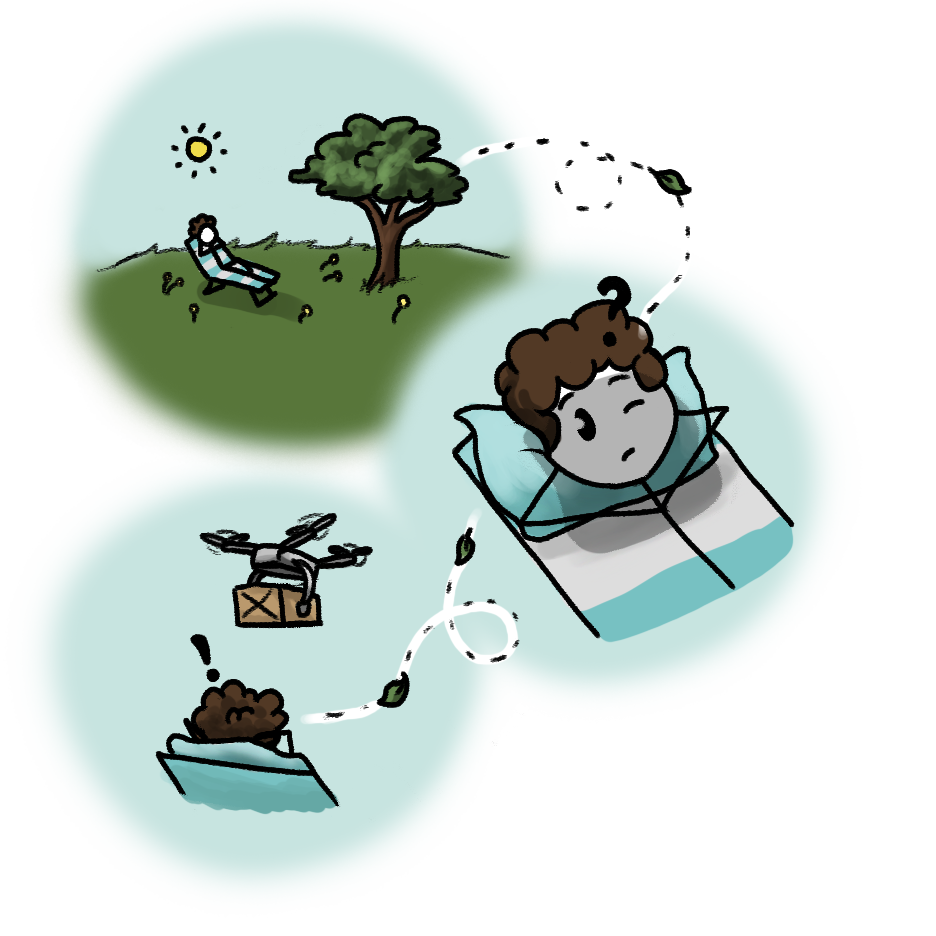
\includegraphics[width=0.9\linewidth]{./chapters/public/intro.png}}
  \large Our friend's day is quite ruined. \small Illustration by Anna Stephenson
\end{figure}

\narr I actually don't know who they should have told; federal jurisdictional
decisions for nuclear incidents is not the drama being told today. But the
authorities quickly found out and figured that out for themselves.

\begin{shadequote} 

  This turns out to be a misdelivered package, because nuclear terrorists are
  people too\ldots that sometimes make typos. The UFU authorities believe that
  there are many more packages on their way to different locations, but having
  no intel on where to intercept them, they need to know where this material
  came from to locate the terrorist group responsible. They need nuclear
  security experts, and FAST.

\end{shadequote}

\narr \textit{Enter: nuclear security}. This is not to be confused with nuclear
safety, that is, making sure nuclear power reactors behave and do not have
accidents that harm the environment and the beings in it---a more-than-worthy
effort, but not the one being discussed here. The nuclear security enterprise
instead focuses on preventing or mitigating undesirable outcomes of a different
variety, like nuclear terrorism. Nuclear security's goal is keeping all of the
nuclear material in the world inside a regulatory pipeline, so none of it gets
into the hands of people who want to do others harm.

\noindent In this universe:\\ A high profile example of nuclear security at
work, at least on a diplomatic level, is the Joint Comprehensive Plan of
Action\footnote{For more information on the JCPOA, see this
\href{https://www.armscontrol.org/factsheets/JCPOA-at-a-glance}{\color{violet}fact
sheet}}, better known as the Iran nuclear deal. Personal opinions (if you have
them) and recent news (if you've seen it) aside, its purpose is to keep a
closer eye on the country to be sure they aren't developing the capabilities
necessary to make weapons.  Another part of the nuclear security effort is a
strong nuclear forensics capability.  Nuclear forensics begins \textbf{after} a
nuclear incident occurs, which sadly, happens. This incident can be some intact
material drone-delivered to a friend by mistake, or it could be something even
worse, like the detonation of a nuclear weapon. Just in 2019, the International
Atomic Energy Agency confirmed malicious intent for six incidents of trafficked
nuclear material\footnote{Here is the
\href{https://www.iaea.org/sites/default/files/20/02/itdb-factsheet-2020.pdf}{\color{violet}2020
document} that contains this information}.

Most might think of forensics as catching a murderer, but this is more like
catching the nuclear smuggler. Given some nuclear material (a body) and
composition of the material\slash how it was encased and transported (the clues
around it like blood and fingerprints), how\slash from where was the nuclear
material obtained and\slash or smuggled (what conclusions can be drawn about
the murder)?  In both situations, forensics work ideally leads to blaming, with
court-admissible proof, someone for the illegal act. Fingerprints of humans are
important to a murder investigation, and likewise, there are fingerprints of
nuclear materials that can provide their point of origin and\slash or where
they were processed.

\begin{shadequote}

  Slight correction: They need \textbf{nuclear forensics} experts, and FAST. 
  
  These UFU authorities are in luck, since our friend happens to be a hobby
  nuclear forensics scientist! As a citizen scientist, they cannot use actual
  nuclear materials or well-equipped laboratories to test their methods and
  ideas. Our friend instead uses their software development and simulation
  skills to study their favorite topic of attributing mysterious nuclear
  materials to their point of origin. This is now their chance to unveil a
  research method to the authorities and see if they can help prevent a nuclear
  weapon from being detonated in the UFU in time. 
  
  But the authorities are not sure. Some experimental method developed by a
  \sout{grad student} hobby scientist surely wouldn't work? Also, it's not
  validated, so it wouldn't hold up in court. But the race to save lives is on.
  ``What,'' they ask, ``do ya got cookin'?''

\end{shadequote}

\narr I'll tell you all about what our friend has cookin': some steak. But hold
on, I'll get there in a minute.

From a visual inspection, the nuclear material in question has been determined
to be nuclear fuel after it's been loaded into, used in, and removed from a
nuclear reactor. By performing some to-be-discussed nuclear forensics
approaches on this material, we can figure out all of the details of this fuel
related to its creation, time in the reactor, and how long it has been out of
the reactor. 

First, I need to define some terms for you. There are four main concepts that
are covered: \textit{reactor type}, \textit{burnup}, \textit{enrichment}, and
\textit{time since irradiation}.  Ideally, the process of determining these
parameters can pinpoint a sample of nuclear fuel to the exact reactor it came
out of!

\begin{figure}[!htb]
  \centering
  \makebox[\textwidth][c]{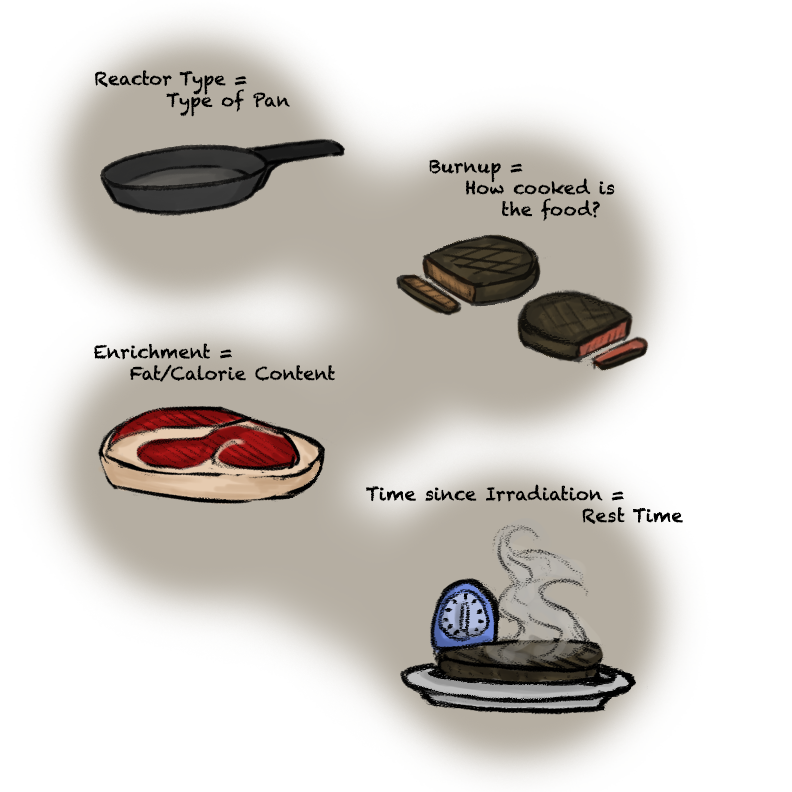
\includegraphics[width=0.9\linewidth]{./chapters/public/nukemetaphor.png}}
  \large If you imagine nuclear fuel as steak, you might be able to figure out 
  the reactor that made it! \small Illustration by Anna Stephenson
\end{figure}

Let's consider the nuclear fuel as food, specifically, steak. We can think of
the reactor as the type of pan our steak was cooked in. If it's cast iron,
it'll make a different steak than a \$10 nonstick pan that's only nonstick for
3 uses (the parallel universe shares some similar woes). The same is true for
nuclear fuel; it looks quite different depending on which reactor type it spent
time in. Our friend focuses on three main types of nuclear reactors, called
\glspl{PWR}, \glspl{BWR}, and \glspl{PHWR}\footnote{We won't cover any details
about these reactors here, but if you're curious about different types of
nuclear reactors,
\href{http://www.world-nuclear.org/uploadedFiles/org/WNA/Publications/Nuclear\_Information/Pocket\%20Guide\%20Reactors.pdf}{\color{violet}here}
is a great summary.}; different countries use one or a mix of these three main
technologies. (More than these three exist, but these are the ones our friend
wants to focus on.) 

There's also a measurement called burnup. In steak-talk, this is how well-done
it is (more accurately, it is how much energy your steak produces, but it is
more ``well-done'' as it cooks longer and produces more energy), and would be
measured in energy produced per unit of raw steak. In nuclear-talk, it's
measured in energy (mega- or gigawatt-days) per metric ton of initial uranium
(MWd/MTU or GWd/MTU). 

Next, the enrichment, meaning \% \gls{U235} enrichment, which refers to how
much of this type of uranium is in the nuclear fuel when it's freshly made.  A
lot of the time, nuclear engineers refer to a specific element from the
periodic table with a mass number attached, like \gls{U235}, as nuclides,
because the concept of nuclides emphasizes nuclear properties, which can differ
drastically even though they are the same element on the periodic table. ``U'' is
shorthand for uranium, and the mass number 235 refers to the number of protons
(92) plus neutrons (143) in the nucleus of the atom. The protons have a
positive charge, and the neutrons have no charge; the protons are balanced by
the negative charge of an equal number of electrons, but we aren't worried
about those right now. \gls{U235} is a special nuclide that nuclear engineers
call \textit{fissile}\footnote{For more information on nuclides and what
fissile means, check out this
\href{https://whatisnuclear.com/isotopes.html}{\color{violet}link}.}: when it
absorbs an extra neutron, it splits into two atoms and releases some energy.
When this energy is harnessed into our electrical grid, it's great, but that
energy can also be harnessed into a weapon, which is not great. This is like
the calorie content or fat content of your steak. The more fat, the more
calories, and so the more energy it can supply. In nuclear fuel, more fissile
material in the form of a higher \gls{U235} enrichment means that the fuel can
provide more energy than a fuel of lower enrichment. Uranium naturally has
0.7\% \gls{U235} in it, but commercial nuclear fuel is commonly enriched up to
5\%.

Last, the time since irradiation measures how long the nuclear fuel, or steak,
has been cooling after it leaves the reactor, or pan. Nuclear fuel is intensely
radioactive when it leaves the reactor, which produces a lot of heat, so it
needs to cool off for a few years to be able to be stored longer term without
heat dissipating measures (which is submerging the nuclear fuel in water; think
of the fuel as taking a several year vacation in a swimming pool). This is just
like our steak needing to rest a little before it's consumed. And that's about
as far as this metaphor can go, because aside from some recent Godzilla movies,
I don't think any of us are eating nuclear waste (in this universe, at least). 

If a nuclear material spent time in a nuclear reactor, these four parameters,
part of what we will call the reactor operation history, are important to
identifying where it came from. Next, we will talk about how identifying
where it came from can happen in an investigation.

\begin{figure}[H]
  \centering
  \makebox[\textwidth][c]{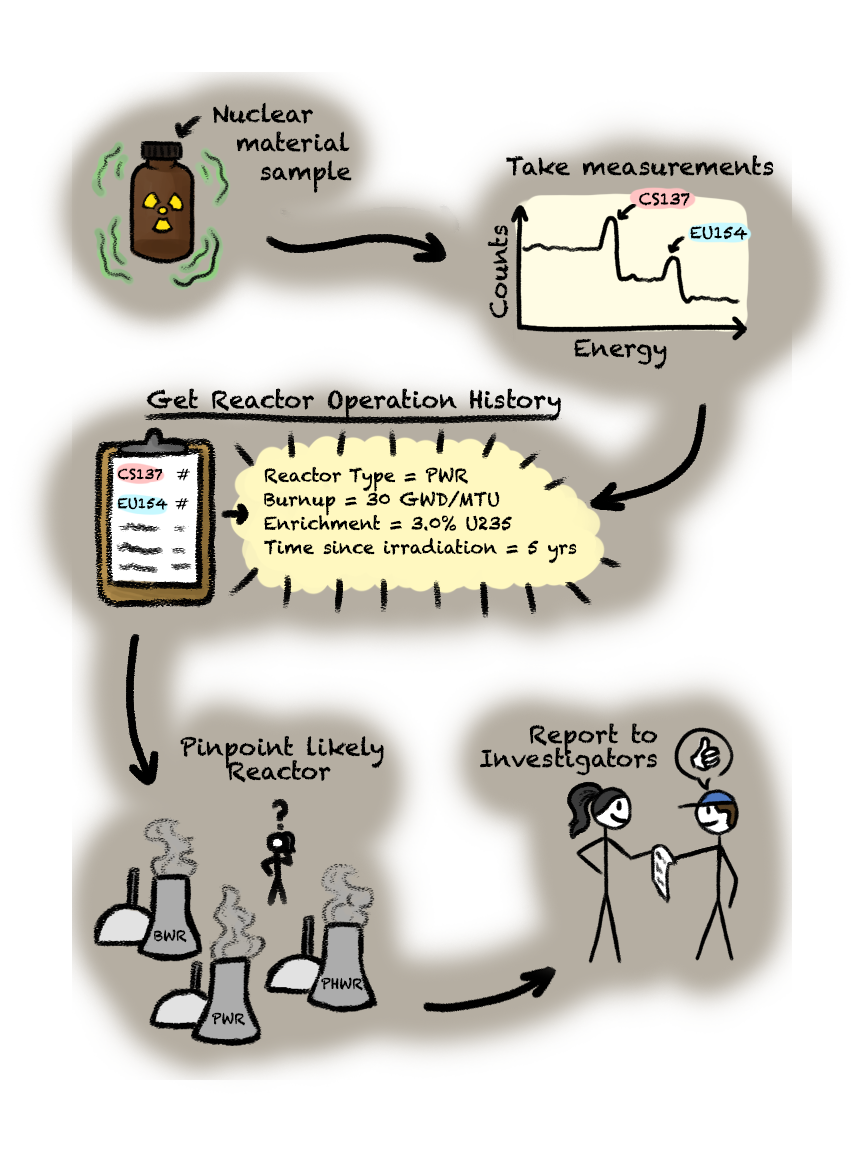
\includegraphics[width=0.8\linewidth]{./chapters/public/nf-workflow.png}}
  \large It's as simple as this $\uparrow$. \small Illustration by Anna Stephenson
\end{figure}

After some of-unknown-origin nuclear material believed to be from a reactor
enters our consciousness, some measurements will be taken by technicians
working with the government. For example, this could be something called
\textit{gamma spectroscopy}, which is pictured in the process below. This
detector measures a type of radioactivity called gamma rays\footnote{Gamma rays
are really cool, and if you read
\href{https://www.symmetrymagazine.org/article/incredible-hulking-facts-about-gamma-rays}{\color{violet}this
article}, you'll think so too!}, and gamma rays have different energies. So the
material is just sitting there spitting out gamma rays left and right and up
and down and the detector is just sitting there measuring the ones that hit it.
It collects counts of gamma rays associated with an energy; this is called a
gamma spectrum. Gamma rays of certain energies are known to come from certain
nuclides. 

Knowing how much of certain radioactive nuclides is in a material can
tell us about the reactor operation history: the reactor type (pan), burnup
(doneness), enrichment (fat), and time since irradiation (rest time). After
determining these parameters, a specialist can pinpoint a specific reactor
somewhere in the world (via access to a reactor history database) that created
the material and investigators can use that to move forward with their work.

\begin{tcolorbox}[halign=center]
\textbf{Methodology}
\end{tcolorbox}

\begin{shadequote}

  In the time it took to get through the lesson above, a foe had enough time to
  arrive on the scene: an official government scientist. This scientist has a
  different priority: precision over speed. Our friend's research is driven by
  ``how fast can I get an answer?'', whereas the scientist is driven by
  ``what's the most correct answer?'' These two priorities in this situation
  are at odds, but both equally important. The authorities need an answer, and
  fast, but it needs to be the right one because otherwise many UFU lives are
  at risk.
  
  Our friend was in the middle of telling the authorities about their fast
  nuclear fuel-identifying machine learning approach when this scientist
  arrived, so they got to listen in:
  
  ``Machine learning is a field under the umbrella of artificial intelligence,
  which allows computers to imitate human behavior. Scientists are using
  machine learning in many fields to solve complex problems, and so I wanted to
  see if it could be useful in my favorite area of study: nuclear forensics.''
  
  Pointing to the top of the diagram, they say, ``So, I first simulated hundreds
  of thousands of examples of nuclear fuel scenarios: different reactor types,
  many levels of burnup, different levels of \gls{U235} enrichment, and times
  since irradiation spanning up to 16 years.  Each simulation gives me lists of
  nuclides and their measurements that are important to determining those four
  parameters.  Machine learning professionals call these lists of nuclides the
  \textit{features}, and the parameters are \textit{labels}. All together, it's
  called a \textit{training data set}.''
  
  Pointing to the middle, ``Next, this training data is put into a
  \textit{machine learning algorithm}\footnotemark[6], which is how people
  teach computers to teach themselves with some software method. Using the
  training data set, the algorithm creates a model, which is usually a model we
  can't see or understand as humans. They are quite secretive creatures, don't
  you think?  Anyway, there are many different types of algorithms, and I have
  tested out some simple ones to see if this approach is even remotely
  feasible. These also happen to be the less-secretive type of algorithms so we
  can understand what the models are doing. One seems to work really well,
  called \gls{MLL} calculations\footnotemark[7], and I think it's good enough
  to use to save UFU.''
  
  Last, they point to the bottom of the diagram. ``So now we have the model. If
  we take the same measurements that exist in the training database features,
  then we can use the model to give us a predicted label, in this case burnup.
  But because I'm doing this experimentally, I know the actual label because I
  simulated this unknown nuclear material. So in this way, I can measure the
  prediction errors and refine my method.''
  
\end{shadequote}

\begin{figure}[H]
  \centering
  \makebox[\textwidth][c]{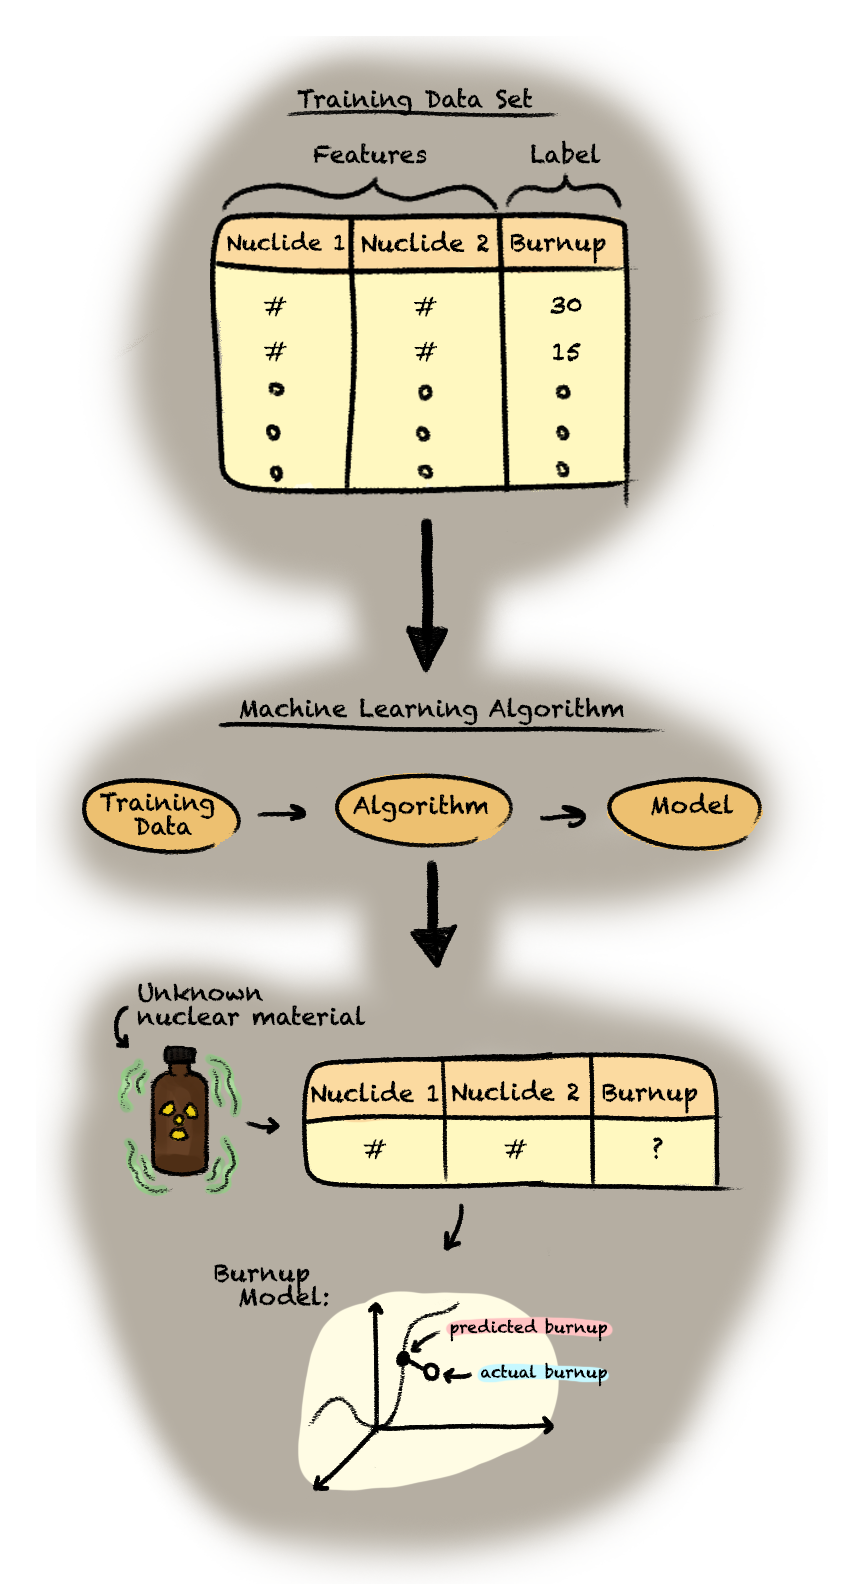
\includegraphics[height=0.9\textheight]{./chapters/public/ml-workflow.png}}
  \large Again, it's as simple as this $\uparrow$. \small Illustration by Anna Stephenson
\end{figure}

\begin{shadequote}

  The UFU authorities' eyes glazed over, but the scientist was excited. They
  were thinking, ``My oh my, we could use this! I have a database just like this
  of the most perfect simulated nuclide measurements that I can use back at the
  lab! I never really knew what to do with it, so I took a screenshot of a few
  entries and used it as my desktop background; databases are beautiful.''
  
  But our friend didn't think the scientist could take the proper measurements
  in time. Our friend uses this method with a different kind of training set,
  one that is created by simulating detectors that can take measurements in
  minutes \textit{(Narrator: remember the gamma spectroscopy from above?)},
  with the expectation that this would help in a real world scenario like this
  one. The gamma detectors measure the radioactivity of the sample, which is
  more difficult to get a direct answer from than the scientist's method in the
  lab, but our friend is all about speed. The measurements the scientist needs
  to take to match the sample with their training database involve dissolving
  the material and making many different measurements of the nuclides using a
  technique called mass spectrometry\footnotemark[8].  It gives super accurate
  results that will do well with the machine learning method, but the
  measurements take weeks. 
  
  They fought about this for about an hour, which was silly because our friend
  could have taken the gamma measurements in a fraction of that time and been
  off to use their machine learning model. But, tensions were high, egos were
  flaring, and everyone wanted to save lives. 
  
  The UFU authorities deglazed their eyes and looked at each other, then at our
  friend, then at the scientist. After some telepathic decision making, they
  said, ``We choose\ldots\ldots''

\end{shadequote}
\footnotetext[6]{For a better introduction to machine learning, read
\href{https://towardsdatascience.com/introduction-to-machine-learning-for-beginners-eed6024fdb08}{\color{violet}this}!}
\footnotetext[7]{If you have institutional access to journals,
\href{https://www.tandfonline.com/doi/full/10.1080/00295450.2017.1401442}{\color{violet}here's
the method's first paper}.}
\footnotetext[8]{I tried to find a non-company-affiliated source that explained
this simply, but failed.
\href{https://www.jeolusa.com/RESOURCES/Analytical-Instruments/Mass-Spectrometry-Basics}{\color{violet}This
is a good explanation}, though, if you're curious about mass spectrometry.}

\vspace{5mm}
\narr Now, you, curious companion, must choose your own adventure. Do we use
our friend's speedy strategy or do we trust the scientist's careful course of
action? Remember, we want to be fast, which our friend can most likely do, but
we also want to be right, which the scientist can most likely do.

\vspace{-13mm}
\begin{figure}[H]
  \centering
  \makebox[\textwidth][c]{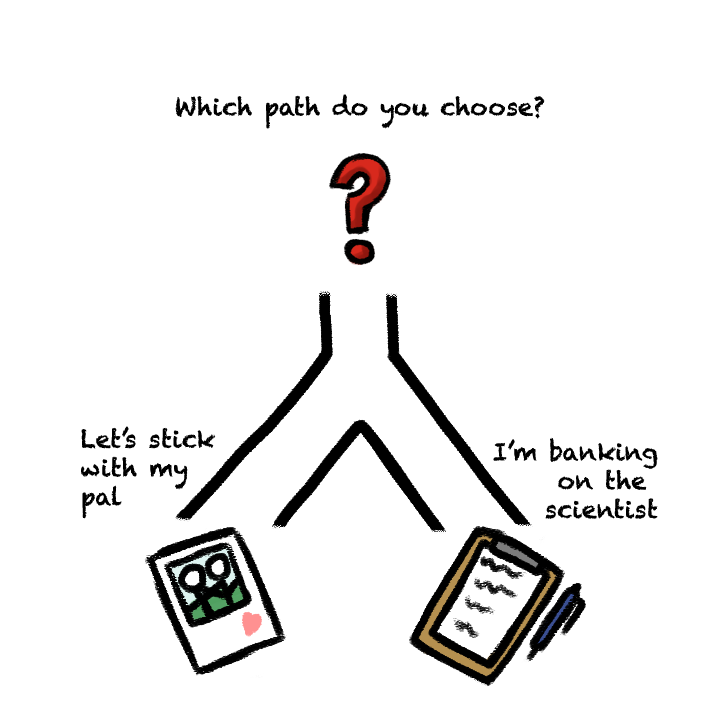
\includegraphics[width=0.69\linewidth]{./chapters/public/path.png}}
  \small Illustration by Anna Stephenson
\end{figure}
\vspace{-6mm}

\noindent \fcolorbox{gray!10}{gray!10}{
  \begin{minipage}[t]{0.45\textwidth}
    
    \setlength{\parskip}{1em}

    ``\ldots our friend!'' Now the race is on to measure the material with a
    gamma detector and predict the fuel's reactor operation history. For a
    hobbyist, our friend has a pretty great gamma detector: a portable
    high-purity germanium detector. It can detect the gamma rays very
    precisely, and our friend always wants to use the best detector they can
    get their hands on.

  \end{minipage}%
}
  \hfill\vline\hfill
\noindent \fcolorbox{gray!10}{gray!10}{
  \begin{minipage}[t]{0.45\textwidth}
  
    \setlength{\parskip}{1em}

    ``\ldots the scientist!'' Now the scientist takes the nuclear fuel to start
    making measurements. Back in their fancy state-of-the-art lab with all the
    mass spectrometry equipment a radiochemist could ever dream of, the
    scientist and their team get started. One week goes by, two weeks go by.
    And by the third week the scientist and their team had measured 29 nuclides
    in the nuclear fuel sample to high precision! 

  \end{minipage}
}

\noindent \fcolorbox{gray!10}{gray!10}{
  \begin{minipage}[t]{0.45\textwidth}
    
    \setlength{\parskip}{1em}

    \vspace{-22pt}
    \begin{figure}[H]
      \centering
      \makebox[\textwidth][c]{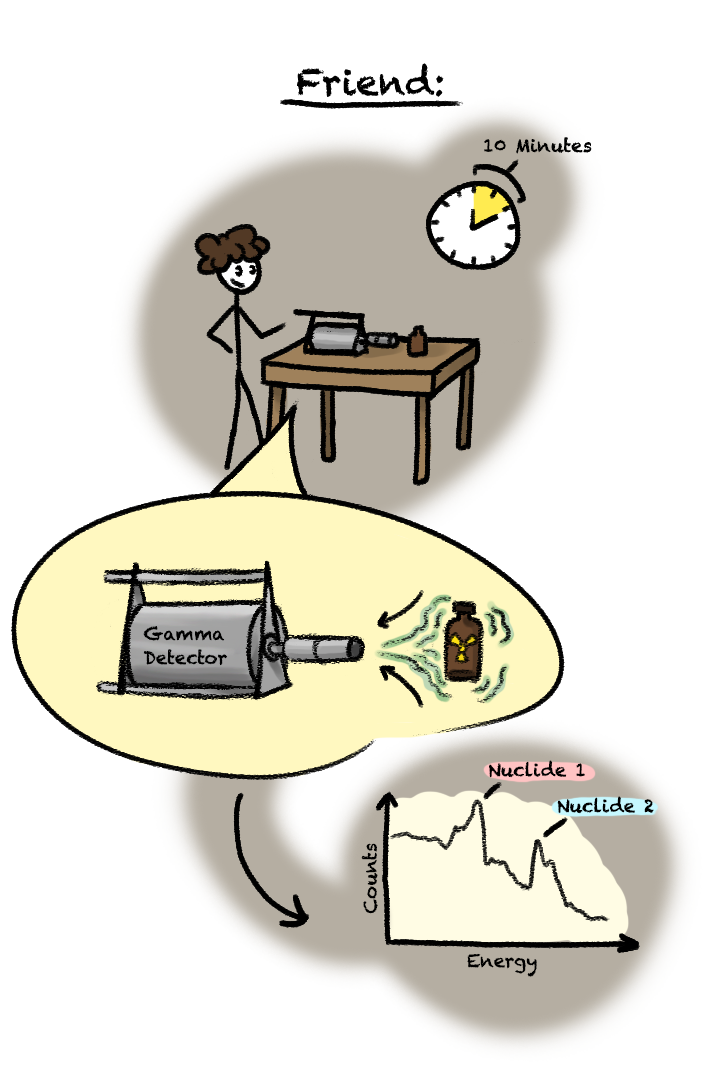
\includegraphics[width=0.95\linewidth]{./chapters/public/gamma_spec.png}}
      \large This process doesn't require advanced training. 
      \small Illustration by Anna Stephenson
    \end{figure}
    \vspace{-7mm}
    
    Using the technical assistance of the UFU authorities, our friend was able
    to protect themself against radiation and take the sample out of its
    packaging to get the best measurements possible. They let the detector
    measure the sample for 10 minutes, et voil\`{a}: a gamma spectrum of the
    sample. Our friend then took the gamma spectrum and compared it against
    their machine-learned model that was created using a training set composed
    of $450,000$ simulated gamma spectra of different types of nuclear fuel.
    And out popped an answer:
  
  \end{minipage}%
}
  \hfill\vline\hfill
\noindent \fcolorbox{gray!10}{gray!10}{
  \begin{minipage}[t]{0.45\textwidth}
  
    \setlength{\parskip}{1em}
    
    \vspace{-46pt}
    \begin{figure}[H]
      \centering
      \makebox[\textwidth][c]{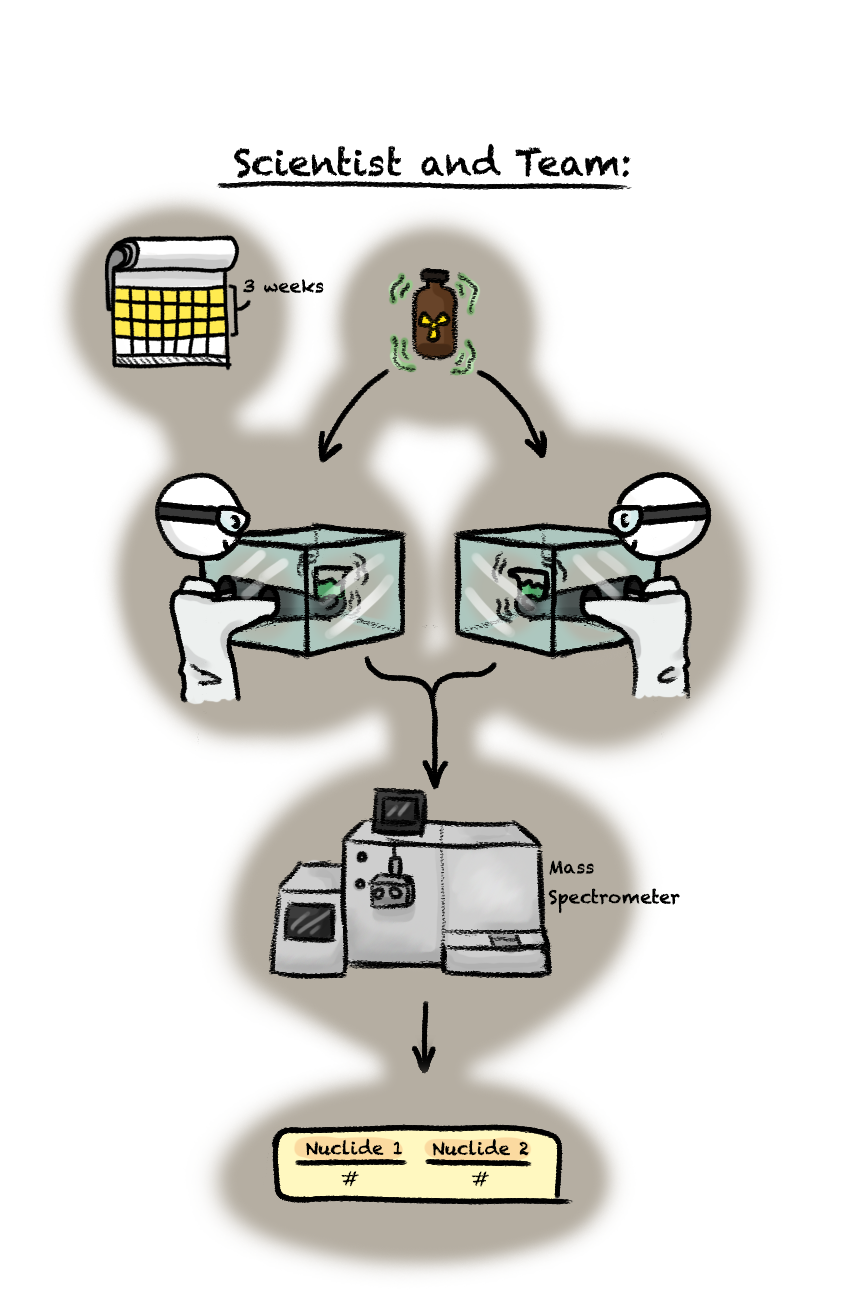
\includegraphics[width=1.2\linewidth]{./chapters/public/mass_spec.png}}
      \large This process is complicated, but here are some snapshots. 
      \small Illustration by Anna Stephenson
    \end{figure}
    \vspace{-7mm}
    
    Now they were ready to borrow our friend's machine learning method to
    predict the parameters of the reactor operation history.  The scientist
    then took the list of 29 nuclides and their measurements and compared that
    information against their machine-learned model that was created using a
    training set composed of $450,000$ of the exact same 29 simulated
    measurements of different types of nuclear fuel. And out popped an answer:
    
  \end{minipage}
}

\begin{tcolorbox}[halign=center]
\textbf{Results}
\end{tcolorbox}
\vspace{-4mm}

\fcolorbox{gray!10}{gray!10}{
  \begin{minipage}[t]{0.45\textwidth}
    
    \setlength{\parskip}{1em}
    
    \begin{table}[H]
      \centering
      \begin{tabular}{ll} \toprule
        Reactor Type     & BWR                          \\
        Burnup           & 44.02 $\scriptstyle GWd/MTU$ \\
        Enrichment       & 2.04 \%\:${}^{235}\text{U}$  \\
        Time Since Irrad & 5.34 $years$                 \\ \bottomrule
      \end{tabular}
    \end{table}
    \vspace{-2mm}
    
    ``Ok! We got it!'' said our friend. Given these values, some of the UFU
    authorities specializing in worldwide reactor operational history databases
    were able to determine this came from a reactor in the Democratic People's
    Republic of Thoria (DPRT). 
    
  
    This made sense to everyone because the DPRT had been a threat for some
    time. Everyone knew their missiles couldn't get to the UFU, so they must
    have concocted a different plan.

    It was a matter of hours before the UFU had hundreds of DPRT conspirators
    in custody. With the culprits contained, the drone-delivered material
    didn't make it to the bomb assembly location, and the day was saved!
    
    \ldots Except, three weeks later, the capital city of Curiumville was
    bombed.
  
  \end{minipage}%
}
  \hfill\vline\hfill
\fcolorbox{gray!10}{gray!10}{
  \begin{minipage}[t]{0.45\textwidth}
    
    \setlength{\parskip}{1em}
  
    \begin{table}[H]
      \centering
      \begin{tabular}{ll} \toprule
        Reactor Type     & BWR                          \\
        Burnup           & 44.02 $\scriptstyle GWd/MTU$ \\
        Enrichment       & 4.11 \%\:${}^{235}\text{U}$  \\
        Time Since Irrad & 4.65 $years$                 \\ \bottomrule
      \end{tabular}
    \end{table}
    \vspace{-2mm}

    ``Ok! We got it!'' said the scientist. Given these values, some of the UFU
    authorities specializing in worldwide reactor operational history databases
    were able to determine this came from a reactor in \ldots GASP! 

    The Commonwealth of Puerto Plutonio, a Territory of the UFU?! This made no
    sense! We thought they liked being colonized!

    It was now a rush to track down the conspirators since there wasn't much
    intelligence data on them. The UFU was scrambling. 

    And in the middle of the scramble, the capital city of Curiumville was
    bombed.
  
  \end{minipage}
}

\vspace{4mm}

\narr Now, curious companion, you are both permitted and encouraged to read the
other adventure. 

After weeks went by the UFU authorities with the help of the scientist were
able to confirm the actual parameters:
\vspace{8mm}
\begin{table}[H]
  \centering
  \begin{tabular}{ll} \toprule
    Reactor Type           & BWR                         \\
    Burnup                 & 44.02 $GWd/MTU$             \\
    Enrichment             & 4.11 \%\:${}^{235}\text{U}$ \\
    Time Since Irradiation & 4.86 $years$                \\ \bottomrule
  \end{tabular}
\end{table}

Our friend's experimental machine learning method isn't so bad for a method
developed with little resources!  Their gamma spectroscopy-based approach
predicted the correct reactor type and burnup.  Most significantly, though,
their method did not predict the \gls{U235} enrichment well, and this is what
led to the false blame on the DPRT.  (The time since irradiation was also 6
months too long, but didn't heavily impact the false attribution like the
enrichment did.) The scientist's mass spectrometry-based approach was clearly
more accurate for all four parameters. The reactor type, burnup, and enrichment
were correctly predicted. Although the time since irradiation was off by 2-3
months, this error didn't result in any false blame being allocated.

In both versions, luckily, the bomb didn't detonate and no one died. It was too
rushed of a job, and with the nuclear test ban treaty, no one actually knows
their nuclear weapons WILL work. You didn't think our friend's tale was going
that dark, did you?

\vspace{8mm}
\begin{shadequote}

  ``Hey,'' the scientist said to our friend, ``I'm famished.'' Our friend said, ``Oh
  goodness, me too!'' They looked at each other, and after some telepathic
  decision making, agreed on a nice steak.

\end{shadequote}

\begin{figure}[H]
  \centering
  \makebox[\textwidth][c]{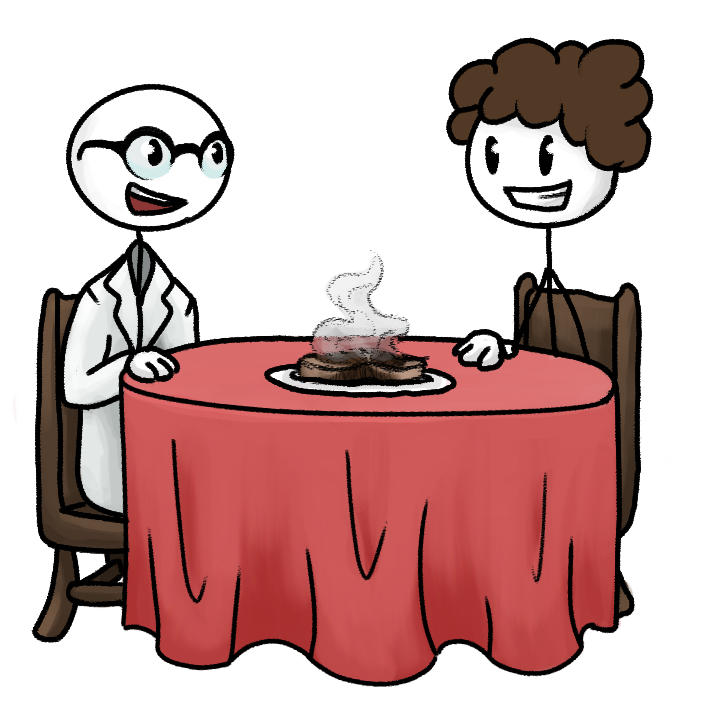
\includegraphics[width=0.75\linewidth]{./chapters/public/theend.png}}
  \large The end. \small Illustration by Anna Stephenson \\~\\
\end{figure}

\hrule

\begin{tcolorbox}[halign=center]
\textbf{Discussion \& Conclusions}
\end{tcolorbox}

This machine learning-based research protocol is designed to answer the
question: \textit{How does the ability to determine forensic-relevant spent
nuclear fuel attributes using machine-learning techniques degrade as less
information is available?} The dissertation written after this chapter answers
that in much more detail than the two scenarios presented here, but I hope to
have communicated the basics of what I'm doing to a general audience. I
actually don't use any real-measured samples by which to compare the different
types of training sets (the samples in this story are a part of my work, but
simulated), but I do use a real-world set of test cases with the 29 nuclide
mass training set.  There are many challenges with doing this yet to be
resolved, so it is not presented here in a research snapshot.

The lack of a feel-good resolution in this tale is not meant to reduce
confidence in our national nuclear forensics capability or my research project,
but rather to show how science does not necessarily result in clear-cut answers
to questions. Much of the time, asking a question and answering it using the
scientific method creates more questions than answers. For example,  there are
questions about why the gamma spectra approach gave such a wrong enrichment
prediction (something echoed in my results, which are aggregate statistics of
$450,000$ cases versus the one case presented here). Another question might be
whether a 3-month or 6-month time since irradiation prediction error is too
large of an error, or an acceptable error.

\begin{tcolorbox}[halign=center]
\textbf{Author Commentary}
\end{tcolorbox}

\textit{Last, I wanted to make a short statement about my work on an even
broader scale.}

Every scientist should take note of the ethical and political implications of
their work. Yes, I said it: science is political\footnote[9]{Everyone knows
\href{https://www.scientificamerican.com/article/yes-science-is-political/}{\color{violet}it}!}!
Although the morality of preventing or mitigating a nuclear disaster is not
necessarily in question, the nuclear field (both commercial power and
defense/the nuclear weapon program) is far from blameless when it comes to
destroying human bodies and the environment. The mining industry caused uranium
contamination and early death for many Din\'{e} in Navajo Nation and
payouts/cleanup only began recently\footnote[10]{For more information about the
500 abandoned mines and the cleanup efforts, read more
\href{https://www.epa.gov/navajo-nation-uranium-cleanup/abandoned-mines-cleanup}{\color{violet}here}.},
plutonium production during World War II has resulted in the displacement and
illness of US citizens around Hanford, WA, and government-sanctioned human
radiation experiments were conducted on unwitting people and children. None of
this (and so much more that's not mentioned here) comes as a surprise knowing
the entire nuclear enterprise sits on a foundation of well-documented
racism\footnote[11]{\href{https://thebulletin.org/2020/08/a-call-for-antiracist-action-and-accountability-in-the-us-nuclear-community/}{\color{violet}Here's}
a good article on nuclear's racist roots.}.  Last, the obvious must be stated:
the US is the only country to ever deploy a nuclear weapon against another
country, where the human toll was undeniably brutal\footnote[12]{And Black
American journalists
\href{https://www.nytimes.com/2021/08/09/science/charles-loeb-atomic-bomb.html?smid=url-share
}{\color{violet}exposed the government's lies} about it}. This and much more is
documented in a list of resources curated by Kalin Kiesling with help from the
nuclear community\footnote[13]{The resources are curated in
\href{https://docs.google.com/document/d/e/2PACX-1vQuRSix5J31G4yhH-Z0kwmlpXe6OgS9MXg6l-LBEOVNDPDAPVivPSrJ7A71TMCsW2EdvGMepZCcwdTP/pub}{\color{violet}this
Google document}.}.

None of this means that nuclear power as an energy source is inherently evil,
but the industry and our government must acknowledge and take responsibility
for abusing both the land and the beings on it. It is hard to hold this
knowledge and still want to participate in nuclear science, but if more people
in nuclear science and industry also hold this knowledge, then maybe taking
life and land for granted can be less of a norm. Of course, better policy is
always a stronger influence. Why am I saying all of this inside a(n unofficial)
chapter in a nuclear engineering dissertation? Science is political, and so I
must be too.  

}

\chapter{Introduction}
\label{ch:intro}

The realm of nuclear security involves parallel efforts in nonproliferation
(verification of treaty compliance, monitoring for smuggling, proper storage
and transportation of nuclear materials), cyber security, minimizing stocks of
weaponizable materials, disaster response training, and nuclear forensics. All
of these efforts have been continually improving, but there was a gap regarding
the ability of the \gls{US} to coordinate and respond to a nuclear incident,
especially with the technical portion of nuclear forensics: characterization
and analysis. After all, the first textbook on the topic was published in 2005
\cite{nftext_2005}. In 2006, the \gls{US} \gls{DHS} founded the \gls{NTNFC}
within the \gls{DNDO}. The mission of the \gls{NTNFC} is to establish a robust
nuclear forensics capability to attribute radioactive materials with
demonstrable proof.

Multiple fields contribute to a nuclear forensics capability, such as
radiochemical separations, material collection techniques, detector technology,
material library development, and identifying forensic signatures. These needs
vary based on whether the material being collected is post-detonation (e.g.,
bomb debris) or pre-detonation (e.g., \glsreset{SNF}).  In the pre-detonation
realm, this project focuses on statistical methods to to model \gls{SNF}
production history using nondestructive detector measurements. 

\section{Motivation}
\label{sec:motivation}

Nuclear forensics is an important aspect of deterring nuclear terrorism even
though it is not, at first glance, obvious preventative nuclear security.  The
most common defense of the field is that nuclear forensics deters state actors,
not terrorist organizations. While it is true that a strong capability
encourages governments to be more active in prevention of nuclear terrorism, it
can also deter the terrorist organizations as well by increasing their chances
of failure. Small destructive successes tend to be more valued than high-risk
mass destruction. Nuclear forensics can also assist in cutting off certain
suppliers of nuclear materials or technologies (e.g., nuclear specialists that
are only involved for financial reasons, access to state suppliers), building a
concrete barrier to nuclear terrorism.  Therefore, nuclear forensics is
considered to impede nuclear terrorism in both tangible and abstract ways
\cite{aps_aaas_forensics}.

Following the prevention value of nuclear forensics, it is important to
understand the process of the technical portion of the investigation and how
that can be improved.  In the event of a nuclear incident, such as the
retrieval of stolen \gls{SNM} or the detonation of a dirty bomb, it is
necessary to learn as much as possible about the source of the materials in a
timely manner. In the case of non-detonated \gls{SNM}, knowing the processes
that produced it is crucial to determine the chain of custody of the
interdicted material.  Section \ref{sec:nfneeds} covers the specific needs of
the nuclear forensics community for \gls{SNF} provenance, and Section
\ref{sec:statscontrib} discusses how computational approaches are useful, with
a focus on why statistical methods in particular are being pursued. 

\subsection{Needs in Nuclear Forensics}

\begin{frame}
  \frametitle{Nuclear Forensics Investigations}
  \begin{minipage}[t]{0.5\textwidth}
    \textbf{Post-detonation}
    \begin{itemize}
      \item Collection: debris, swipe samples
      \item Characterization: rapid analysis of isotope ratios
      \item Goals
      \begin{itemize}
        \item Inverse problem: reconstruct weapon design/yield
        \item Safety: informing disaster response
      \end{itemize}
      \item Data evaluation
    \end{itemize}
  \end{minipage}%
  \pause
  \begin{minipage}[t]{0.5\textwidth}
    \textbf{Pre-detonation}
    \begin{itemize}
      \item Collection: depends on intercepted material
      \item \boxalert{Characterization:} non-destructive and destructive
      \item Goals:
      \begin{itemize}
        \item \boxalert{Inverse problem:} material chain of custody
        \item Safety: material handling and security
      \end{itemize}
      \item \boxalert{Data evaluation}
    \end{itemize}
  \end{minipage}
\end{frame}


\begin{frame}
  \frametitle{Nuclear Forensics as an Inverse Problem}
  Necessary to determine the quality of prediction

  Use Bayes' Framework:
  $$ P(A|B) = \frac{P(B|A)P(A)}{P(B)} $$
  $$ P(M|D) = \frac{P(D|M)P(M)}{P(D)} $$
\end{frame}


\label{sec:nfneeds}

\subsection{Contribution of Statistical Methods}
As previously mentioned, there are two main issues that are being addressed for
forensics of \gls{SNF}: database issues and speed of characterization. Many
have begun considering computational approaches to nuclear forensics problems,
such as the INDEPTH tool for inverse depletion and decay analysis
\cite{weber_2006, weber_2010, weber_2011}. This tool uses an iterative
optimization method involving many forward simulations to obtain reactor
parameters of interest given some initial values. 

Another approach utilizes artificial intelligence to solve nuclear forensics
problems, such as implementing searching algorithms for the database comparison
step \cite{gey_search} and machine learning for determining reactor parameters
from \gls{SNF} characteristics \cite{dayman_feasibility_2013, nicolaou_2006,
nicolaou_2009, nicolaou_2014, robel_2009, jones_viz_2014, jones_snf_2014}.  A
variety of statistical and machine learning tools have been used to
characterize spent fuel by predicting categories or labels (reactor type, fuel
type) as well as predicting values (burnup, initial enrichment, or cooling
time) The former uses classification algorithms and the latter uses regression
algorithms. Many algorithms can be applied to both cases.

A typical (supervised) machine learning workflow would take a set of training
data with labels or values inserted into some statistical learner, calculate
some objective, minimize or maximize that objective, and provide some model
based on that output. Then a test set (with known values) is provided to the
model so that its performance can be evaluated and finalized. After model
finalization, a user can provide a single instance and a value can be predicted
from that. \todo{insert ML schematic}

To obtain reliable models, one must 1. choose/create a training set carefully
and 2. study the impact of various algorithm parameters on the error. Many
algorithms are developed on an assumption that the training set will be
independent and identially distributed (i.i.d.). [Aside: there are ways to
handle skewed data sets] This is important so that the model does not overvalue
or overfit a certain area in the training space. Additionally, algorithm
performance (or error) can be optimized with respect to training set size,
number of features, or algorithm parameters (regularization terms, etc).  These
are known as diagnostic plots. When plotting the training and testing error
with respect to the number of instances, this is known as a learning curve.
When plotting these errors with respect to the number or features or algorithm
parameters, this is known as a validation curve. \todo{insert example
diagnostic plot?}

Algorithm choice is usually based on what is being predicted and intuition
regarding strengths and weaknesses.  For the sake of comparison (i.e. weak
validation), some machine learning approaches here are based on previous work
\cite{dayman_feasibility_2013} while also extending to a more complex model
via an algorithm that is known to handle highly dimensional data sets well.
Thus, this paper investigates three regression algorithms: nearest neighbor,
ridge, and support vectors.


It is first important to determine if statistical methods can
overcome the inherent database deficiencies. Next, the statistical methods must
be considered in such a way as to represent a real-world scenario. Although
mass spectrometry techniques provide extremely accurate isotopic information
for analytical methods, they are time-consuming and more expensive. And
although gamma spectroscopy can give extremely fast results cheaply, it only
measures certain radiological signals and is influenced by many environmental
factors, storage, and self-attenuation. As different machine learning
algorithms and parameters are investigated, this work focuses on probing the
amount of information required to obtain realistic results.

Because creating databases from real measurements to represent reactor
technologies from around the world is impossible, the database in this study
will be created from high-fidelity simulations via ORIGEN irradiation and
depletion \todo{check actual name of code part used}. In the simulation and
statistical learning paradigm, we need to determine how much information to
what quality is needed to train a machine-learned model; the model must give
appropriate predictions of reactor parameters given a set of measurements from
a test sample of interdicted \gls{SNF}. Of interest to an entity trying to
create a weapon is partially irradiated fuel if they have plutonium separations
capabilities or any radioactive substance in the case of a dirty bomb.
Addressing the former, a set of simulations of \gls{SNF} at different burnups
and cooling times will comprise the database.\todo{rewrite to be clearer}

Can the algorithm overcome the deficiencies of gamma detection and still
provide useful results? Or does it need more information, e.g., exact
isotopics? First, we must establish some baseline expectations of reactor
parameter prediction and how different algorithms perform. This work is based
off previous work on the subject \cite{dayman_feasibility_2013} regarding
machine learning performace with respect to information reduction, and expands
upon it by also evaluating a more advanced machine learning algorithm: support
vector regression. 



Below is a more in depth discussion of nuclear forensics and
how machine learning can contribute to this research area. After that, an
experimental design is outlined. Lastly, the results are presented and
discussed. 

Thus, ultimately, the goal is to answer the question \textit{How
does the ability to determine forensic-relevant spent nuclear fuel attributes
degrade as less information is available?}. 

%%%%%



\label{sec:statscontrib}

\section{Methodology}
\label{sec:methodology}

As previously mentioned, the typical workflow of the technical portion of a
forensics investigation is to analyze measurements of an unknown material. The
measurements are compared to databases filled with previously measured standard
materials with known reactor parameters, and/or the reactor parameters are
calculated from empirical relationships.  As this work focuses on \gls{SNF},
these measurements are elemental, chemical, and radiological in nature.
Because creating databases from real measurements to represent \gls{SNF} from
reactor technologies from around the world is not within the scope of this
project, the database in this study will be created from high-fidelity
simulations via the \gls{SCALE} \cite{scale} system using \gls{ORIGEN}
\cite{origen}. 


To understand how a physics-free model can predict nuclear reactor parameters,
Figure \ref{fig:compworkflow} introduces the \gls{INDEPTH} and statistical
methodologies, both of which use simulated \gls{SNF}.  While not all steps are
required to be equivalent, the only difference here is the method one chooses
to obtain reactor parameters. Both workflows address speed of characterization,
as it is intended to have gamma spectra as the inputs.  Because \gls{INDEPTH}
is better studied and validated than statistical methods \cite{weber_2006,
weber_2011, weber_2010}, this work focuses on a statistical approach but with
the intention to compare methodologies.  Both workflows also address many of
the database issues, described above. The statistical methodology is described
below.
\\
\begin{figure}[!tbh]
  \makebox[\textwidth][c]{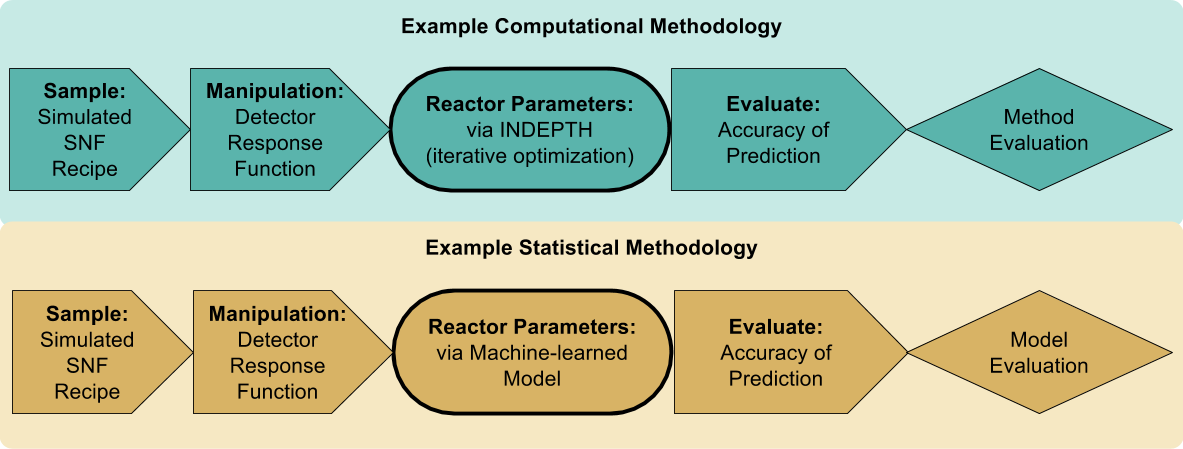
\includegraphics[width=\linewidth]{./chapters/intro/CompStatForensicsWorkflow.png}}
  \caption{Computational Forensics Research Workflows}
  \label{fig:compworkflow}
\end{figure}

In the simulation and statistical learning paradigm, we need to determine how
much information to what quality is needed to train an \gls{ML} model;
the model must give appropriate predictions of reactor parameters given a set
of measurements from a \textit{test} sample. 

The next step is to choose an algorithm that performs statistical learning.
Statistical learners have varied strengths and weaknesses based on what is
being predicted and how they implement optimization.  Chosen for this study are
simple regression algorithms for burnup prediction: nearest neighbor and ridge
regression.  For comparison, \acrfull{SVR} is used because it is known to handle
highly dimensional data sets well.  These algorithms are introduced in Section
\ref{sec:algs}.

After the training is complete, the results of each models' predictions must be
evaluated according to \gls{ML} best practices.  The machine-learned
model predicts the parameters of a previously unseen test set.  The difference
between the model predictions and the actual simulated parameters is known as
the testing error.  The testing error with respect to various specifications
such as the training set size, number of features, or algorithm parameters
provides insight into the model performance. These results are broadly known as
diagnostic plots and show if the predictions are due to good performance or bad
fitting. 

After the models are evaluated, it will be important to compare them both
against each other and against other computational forensics methods. Thus, a
Bayesian approach from the field of inverse problem theory will be used to give
the probability distribution of the predictions so that the statistically
generated predictions can be evaluated directly against other solutions, such
as the optimization-based method, \gls{INDEPTH}. 

Next, information reduction (within the training and testing data sets) must be
used to investigate the extension of this workflow to the real world. The
primary example here is the reduction of information quality via gamma ray
detectors.  If an algorithm could overcome the limitations of gamma detection
and still provide useful results, this would warrant further studies and
perhaps be field-applicable.

Thus, ultimately, the goal is to answer the question \textit{How does the
ability to determine forensic-relevant spent nuclear fuel attributes using
machine learning techniques degrade as less information is available?}. 

\section{Goals}

The main purpose of this work is to evaluate the utility of statistical methods
as an approach to determine nuclear forensics-relevant quantities as less
information is available. \Gls{ML} algorithms are used to train models
to provide these values (e.g., reactor type, time since irradiation, burnup)
from the available information. The training data is simulated using
\gls{ORIGEN}, which provides an array of nuclide concentrations as the features
($X$) and the parameters of interest ($y$) are provided from the simulation
inputs.  Information reduction is carried out using computationally generated
gamma spectra; the radionuclide concentrations from the simulations can be
converted into gamma energies, which then undergo a detector response
calculation to represent real as-measured gamma spectra as closely as possible.
\Gls{ML} best practices are used to evaluate the performance of the
chosen algorithms, and inverse problem theory is used to provide an interval of
confidence in the model predictions.

The necessary background is covered in Chapter \ref{ch:litrev}.  First, an
introduction to the broader field of nuclear forensics is in Section
\ref{sec:nfoverview} to place this work in the context of the technical mission
areas. After that, a short discussion of the field of \gls{ML}, the
algorithms used, and validation methods are in Section \ref{sec:mlback}.
Section \ref{sec:fcsim} includes information about the software used to generate
the training data and perform the predictions. Lastly, a review of statistical
methods being used in studies of forensics analysis is covered next in Section
\ref{sec:stats4nf}. 

After the existing work is discussed, the methodology and a demonstration of
the experimental components is introduced next in Chapter \ref{ch:demo_method}.
This will cover the simulated training data in Section \ref{sec:training}, the
the details for training models in Section \ref{sec:statmodel}, and the
process of model evaluation in Section \ref{sec:valid}.  

Finally, Chapter \ref{ch:proposal} summarizes the official thesis research
proposal. After the preparatory tasks are covered in Section \ref{sec:prep},
there are three experiments outlined in Sections \ref{sec:exp1},
\ref{sec:exp2}, and \ref{sec:exp3}. Qualitiative hypotheses as well as
alternative directions for risk mitgation are discussed throughout these
sections.  A detailed explanation of the method comparison step is covered next
in Section \ref{sec:modelcompare}.  Lastly, a projected timeline for the
completion of this project is in Section \ref{sec:timeline}.

\chapter{Background and Literature Review}
\label{ch:litrev}

This chapter provides a background and literature review of the necessary
components for this project. Section \ref{sec:nfoverview} outlines the broader
field of technical nuclear forensics, with a focus on the area that motivates
this project.  Section \ref{sec:mlback} introduces the field of machine
learning for an uninitiated audience, covers the relevant algorithms, and
presents the methods field practitioners use for validation. Next, Section
\ref{sec:fcsim} covers the computational methods used to generate the training
data for the machine learning input. Finally, the marriage of Sections
\ref{sec:nfoverview}, \ref{sec:mlback}, and \ref{sec:fcsim}, is presented in
Section \ref{sec:stats4nf}, which is a review of previous work applying
statistical methods to the nuclear forensics analysis of pre-detonated nuclear
materials. 

\section{Nuclear Forensics}
\label{sec:nfoverview}
Nuclear forensics comprises a large part of an investigation into a nuclear
incident, such as interdicted nuclear material or the detonation of a weapon
containing radioactive components.  The forensics portion of the investigation
encompasses both the analysis of nuclear material and/or related paraphernalia
as well as the interpretation of these results to establish nuclear material
provenance. The former has many technical aspects, relying on a range of
nuclear science and chemistry.  The latter involves intelligence and political
considerations of the material analyses for attribution. This review will only
consider the technical portion of the nuclear forensics workflow.

First discussed are the types of forensic investigations in Section
\ref{sec:types}, followed by an introduction to inverse problem theory in
Section \ref{sec:inverse} as a way to frame the forensics problem.

\subsection{Types of Nuclear Forensics Investigations}
\label{sec:types}

The technical programs researching improvements to the \acrshort{US}'s nuclear
forensics capabilities are split between the type of material being
investigated. The analysis of irradiated debris from a weapon has different
collection and measurement requirements than a mass of \gls{SNM}. This
separates the field into post-detonation and pre-detonation nuclear forensics.
While both are discussed below in Sections \ref{sec:postdet} and
\ref{sec:predet}, respectively, there is more focus on pre-detonation topics
since this work is based on \gls{SNF}.

\subsubsection{Post-Detonation}
\label{sec:postdet}

Post-detonation nuclear forensics requires a diverse set of measurements to
obtain the following information: identification of nuclear material,
reconstruction of the weapon device design, and reactor parameters for nuclear
material provenance. This could apply to an improvised nuclear device or a
nuclear bomb.  In conjunction with the measurements and characterization are a
large array of logistical concerns, including recovery efforts, personnel
safety, and material collection cataloging and transportation.

In the case of a full explosion using fissile material, the collection of
materials and debris occurs as quickly as possible.  It can be in the crater
created by the explosion, further away from the center in the fallout, and in
the atmosphere above or downwind from the detonation. These are collected by
finding glass-like material near the epicenter, debris swipes in the fallout
region, and advanced particle collection in the atmosphere via an airplane,
respectively.  While the epicenter cannot be reached for some time, the debris
and atmosphere measurements of radioactive material can provide the yield of
the weapon and whether it was made using uranium or plutonium. This along with
other physical and chemical measurement allow device reconstruction to begin.
Attribution begins to narrow to specific countries or organizations based on
this information. \cite{aps_aaas_forensics}

The research needs for post-detonation focus on material collection and
analysis as well as nuclear device modeling for reconstruction purposes.
Ideally, most material sample collection would be done using automatic
instrumentation.  Additionally, bolstering the existing device modeling code
for reverse engineering is needed.  And, as with pre-detonation, a database of
standard materials must be both strengthened and centralized.
\cite{aps_aaas_forensics}

\subsubsection{Pre-Detonation}
\label{sec:predet}

Pre-detonation nuclear forensics investigations occur for every scenario in
which non-detonated nuclear material has been found or intercepted. Although
this could be an intact bomb, it is more likely that \gls{SNM} intended for a
weapon would be the target of an investigation. Thus, the range of intact
materials for measurement could be as small as a plutonium sample or as large
as a shipment of \gls{UOC}.  The goal is to determine the provenance of the
\gls{SNM}, which in the case of \gls{SNF} is generally done by reconstructing
the irradiation process that created the material. 

For \gls{SNF}, where the material was obtained is the first step of the
investigation. This would be gleaned from the reactor parameters and storage
history (e.g., reactor type, cooling time, burnup), which requires first
measuring and calculating certain values: isotopic ratios, concentration of
chemical compounds, or existence of trace elements.  Both radiological methods
(e.g., gamma spectroscopy) and ionization methods (e.g., mass spectrometry)
measure these quantities.  

Although this is less of a humanitarian emergency than a post-detonation
investigation, it is still important to have rapid characterization
capabilities via on-site non-destructive analyses.  As previously discussed in
Section \ref{sec:motivation}, however, the faster measurements result in poor
measurement quality. Also, there is a need for research to combat the database
issues, as an insufficient forensics database can reduce the accuracy and/or
certainty of a reconstructed set of reactor parameters.  Another area of
research is deeper study of known forensics signatures or discovering new
signatures with modeling, simulation, or statistical methods. 

\subsection{Nuclear Forensics as an Inverse Problem}
\label{sec:inverse}

Nuclear forensics is a traditional inverse problem, which has been well
documented mathematically and applied to a range of scientific disciplines.
Understanding inverse problem theory can help systematically define the
limitations of certain solution methods.  This section provides an introduction
to the topic as well as its application to nuclear forensics. 

As outlined in a textbook on the formal approach to inverse problem theory
\cite{inverse_theory}, the study of a typical physical system encompasses three
areas:
\begin{enumerate}
  \itemsep-0.75em
  \item \textit{Model parameterization}
  \item \textit{Forward problem:} predict measurement values given model parameters
  \item \textit{Inverse problem:} predict model parameters given measurement values
\end{enumerate}

First, this shows that it is important to consider the parameters that comprise
a model; this is denoted as the \textit{model space}. This is not every
measurable quantity; domain knowledge is necessary to determine the model
space. In the nuclear forensics context for \gls{SNF}, this would consist of
the reactor operation history parameters. For example, this could be the time
since irradiation because the \gls{SNF} decays and material measurements are
different depending on when the measurement is taken.

Second, understanding the physical system also requires an understanding of the
forward problem. Predicting how a certain set of values of model parameters
will affect the resulting measurements is a problem with a unique solution.
The breadth of these end measurements provides the \textit{data space}, which
are all the conceivable results of a given forward problem. So for \gls{SNF}
this would be, e.g., the range of nuclide measurements typical of a commercial
reactor. 

Lastly, the inverse problem is predicting the model parameters (like time since
irradiation) given a solution (like an assay of nuclide measurements).  It is
statistical in nature; there is a probability that the measured nuclides are
caused by some value of a model parameter. Thus, the problem is
\textit{ill-posed} because a prediction is not guaranteed to be unique. 

\cite{inverse_select}
\cite{inverse_compare}

Further, including measurement uncertainties broadens the linear model to
probability densities of the parameters. The opposite is also true in the
forward case: including parameter uncertainties broadens the forward problem
results to probability densities of the potential measurement values.
\cite{inverse_theory}

In this way, we can define some probability that an answer is correct, given a
set of measurements and their uncertainties, the calculated model parameters,
the spread of the data space, and the spread of the model space. Inverse
problem theory connects these values to the general form of Bayes' theorem,
which is commonly expressed as follows:
\begin{equation}
  \label{eq:bayes}
  P(A|B) = \frac{P(B|A)P(A)}{P(B)}
\end{equation}

%Here, $A$ and $B$ are events, $P(A)$ and $P(B)$ are the probabilities that
%events $A$ and $B$ will occur, representing the model and data spaces,
%respectively. $P(A)$ is known as the likelihood and $P(B)$ is known as the
%marginal likelihood. The marginal likelihood is a concept of the data space
%capturing all the possible measurement values. It is ignored here because as a
%homogenous probability, it is only useful for determining absolute
%probabilities and this will only be applied in a relative context.  $P(B|A)$ is
%the prior probability that event $B$ will occur given a known result for $A$,
%which are the measurements given the model parameters (i.e. the forward
%problem).  $P(A|B)$ is the posterior probability that event $A$ will occur
%given a known result for $B$, which are the predicted model parameters given
%the measurements (i.e., the inverse problem) \cite{inverse_theory,
%gentle_bayes}. 

This is can be mapped easily to the inverse physical system problem scenario.
$A$ would represent an occurrence of a parameter in the model space, and $B$
would represent the measurement of some value. Thus, $P(A)$ is the probability
of a parameter existing without any knowledge of $B$. This is known as the
prior probability, usually given by some theory about the system. $P(B)$ is the
probability of some measurement existing without any knowledge of $A$. This is
known as the marginal likelihood, which is some homogeneous concept for the
potential measurements that could be made (this only serves to scale to
absolute probabilities and does not affect the relative probabilities). The
likelihood, $P(B|A)$, is the chance that a measurement is observed from a given
parameter, representing the forward problem.  Lastly, the posterior probability
is the chance of some parameter existing given some measurement, representing
the inverse problem solution \cite{inverse_theory, gentle_bayes}.  

Given the above, it is more intuitive to consider the conceptual version of
Bayes' theorem in Equation \ref{eq:bayes_words}.
\begin{equation}
  \label{eq:bayes_words}
  \text{Posterior} = \frac{\text{Likelihood} \cdot \text{Prior}}
                          {\text{Marginal \ Likelihood}} 
\end{equation} 

This framework is helpful for an experiment that intends to compare different
methods for calculating the posterior probability of a system given some
measurements \cite{bayes_compare}.  In the nuclear forensics context of
pre-detonated materials, this would be a a set of probabilities for different
parameters of interest, e.g., reactor type, burnup, cooling time, and
enrichment of some interdicted \gls{SNF}.


\section{Machine Learning}
\label{sec:mlback}
Machine learning is a sub-field of \gls{AI} within the broad category of
computer science. The goal of \gls{AI} is to create computer systems that
respond to their environment according to some set of criteria or goal. For
example, self-driving vehicles have computers on board that learn to avoid
curbs and humans. While its use has been increasing in the commercial sector,
there is also much anecdotal evidence to support the existence of a rapid
increase of \gls{AI} use in academic research across many disciplines beyond
robotics. \gls{AI} systems have been used in detection (e.g., fraud or spam),
medical diagnostics, user analysis (e.g., Netflix ratings), and a host of
scientific disciplines that have increasing amounts of multivariate data.

Much of the recent advances to the field of \gls{AI} have occured in the
statistical realm, which forgoes domain knowledge in favor of large data sets.
Thus, machine learning and statistical learning have become somewhat separate
fields \cite{changingml}. Machine learning research focuses on the underlying
algorithms using mathematical optimization, methods for pattern recognition,
and computational statistics.  Since this work is only an application of
machine learning, there is no distinction made between the terminology.
Additionally, this study is not concerned with computational time, but rather
the ability to correctly predict values and categories relevant to the nuclear
forensics mission. This restricts the relevancy of the algorithms to the
underlying theory and its impact on the resulting model's accuracy. 

Machine learning algorithms can be separated into two main categories:
unsupervised and supervised learning.  The former groups or interprets a set of
input data, predicting patterns or structures. The latter includes both the
input and output data, enabling the trained model to predict future outputs.
Broadly speaking, the unsupervised learning algorithms are designed for
clustering data sets or dimensionality reduction (i.e., determining some subset
or linear combination of features most relevant to the input data) of data
sets.  Supervised learning algorithms predict both discrete and continuous
values via classification and regression, respectively. Some algorithms can
perform both classification and regression, and neural networks can even be
modified to perform either supervised or unsupervised learning. 
%Additionally, various algorithms can be strung together, which is referred to
%as \textit{ensemble methods}. One common way of doing this is performing
%deimensionality reduction prior to supervised learning
\\
\begin{figure}[!htb]
  \makebox[\textwidth][c]{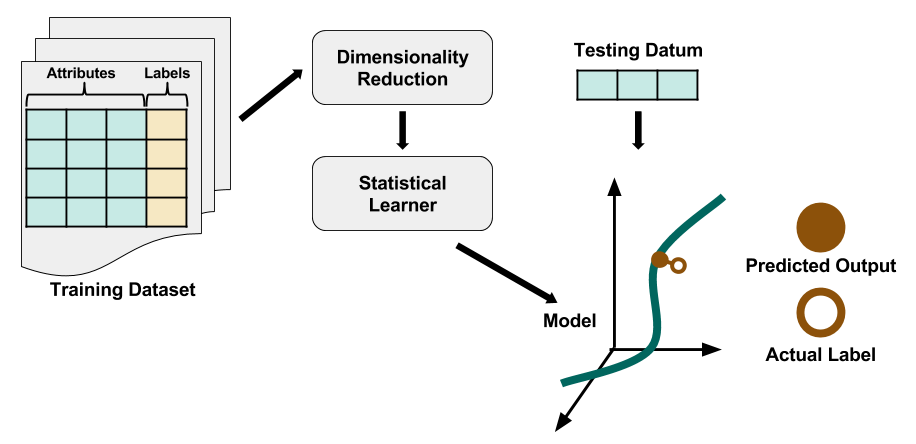
\includegraphics[width=1.15\textwidth]{./chapters/intro/SupervisedRegression.png}}
  \caption{Schematic of Regression with Machine Learning}
  \label{fig:supervised}
\end{figure}

As shown in Figure \ref{fig:supervised}, a typical (supervised) machine
learning workflow begins with a training data set, which has a number of
\textit{instances}, or rows of observations.  Each instance has some
\textit{attributes}, also referred to as \textit{features}, and a label, which
can be a categorical label or discrete/continuous values.  

The training data are then inserted into a statistical learner; this calculates
some objective, minimizes or maximizes that objective, and provides some model.
This model is typically evaluated using a testing set that has the same set of
attributes and labels (but different instances). The comparison of what the
model predicts and the actual label gives the \textit{generalization error}.
Depending on the performance and application, the model may need improvement
from more training and/or some changes in the algorithm parameters. Once the
model is performing well enough and validated, it is finalized; then a user can
provide a single instance and a value can be predicted from that. 

This study performs regression tasks using supervised learning algorithms.
Differences among the underlying mathematics of the algorithms impact the
trained models.  Therefore the algorithms used in this study will be discussed
in Section \ref{sec:algs}. Next, model selection and assessment is covered in
Section \ref{sec:selectass}.  Evaluating and optimizing algorithm performance
is discussed in Section \ref{sec:optvalid}, as well as robustly comparing
different algorithms for validation.

\subsection{Algorithms for Statistical Learning}
\label{sec:algs}
%\setlength\abovedisplayskip{2.5pt}

For relevant nuclear forensics predictions, both classification and regression
algorithms must be used.  For example, one may want to predict the reactor type
label given some measurement-based features of \gls{SNF} of an unknown source.
This would require a classification algorithm. Or perhaps the input fuel
composition is relevant to an investigation on weapons intent, so a regression
algorithm would be used. 

There are three algorithms presented in this section: \textit{k}-nearest
neighbors, decision trees, and \gls{MLL} calculations. They were chosen based
on their simplicity; this work has yet to be benchmarked using simple
algorithms so a more complex treatment of the training sets in this work would
be premature. Additionally, in part because of their simplicity, they are all
"white box" methods.  This is unique in the \gls{ML} universe, since most
algorithms create a black box model that is unable to be analyzed by a human.
The  decision trees method provides an output model that can be used to discern
behavior and understand predictions, and \textit{k}-nearest neighbors and
\gls{MLL} calculations do not create a model at all. Individual predictions can
still be analyzed, however, since the procedures are so simple. 

\subsubsection{Nearest Neighbor Methods}

Nearest neighbors classification and regression are unique algorithms in
that thay are instance-based; they do not actually generalize, but instead
track the observations in the training set.  The main metric for this algorithm
is distance (or dissimilarity) between the test sample and the closest training
sample(s) in the vicinity.  During prediction, the algorithm will calculate a
value based on the instance that is closest to the current test sample. Thus,
there is not any learning, but instead a direct comparison between an unknown
sample and the space that the training set populates. The predictions from
nearest neighbors can be quite accurate, but are highly unstable to
peturbations \cite{elements_stats}.

The process of prediction with \textit{k}-nearest neighbors is as follows.
First, the distances between the test sample and each of the training set
instances are calculated.  Most commonly the Euclidian distance is used, but
this walkthrough uses the Manhattan distance:
\begin{equation}
  d_{i} = \sum_{j=1}^{N_{feats}} |x_{j,train} - x_{j,test}|
  \label{eq:l1}
\end{equation}
where $i$ is each training set instance, and $j$ refers to each feature in the
training set.  The lowest \textit{k} $d_{i}$ are chosen. For \textit{k}-nearest
neighbors regression, the value, $y$ is predicted using the following equation.
\begin{equation}
  y(\boldsymbol{x}) = \frac{1}{k} \sum_{i=1}^{k} w_i \cdot y_i
  \label{eq:knn}
\end{equation}
where $w_{i}$ is either uniform and takes on a value of $1$ or is
distance-based and takes on a value of $1/d_{i}$ and $\boldsymbol{x}$ is the
full set of features. The regression equation averages the closest \textit{k}
neighbors for an estimate of the unknown sample.  In \textit{k}-nearest
neighbors classification, the class label $y$ is predicted using the mode of
the nearest neighbors selected using the \textit{k} smallest $d_i$, or when
$w_i$ is $1/d{i}$ the weighted mode is used to choose the predicted label.

\begin{figure}[!htb]
  \centering
  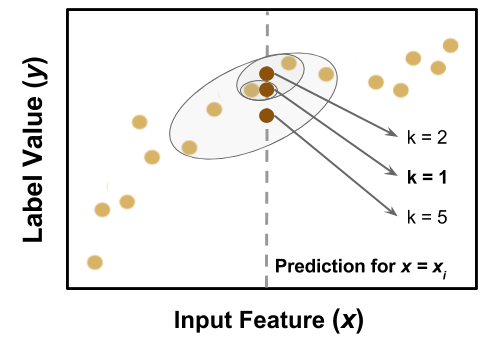
\includegraphics[width=0.8\linewidth]{./chapters/litrev/nn-fig.png}
  \caption{Schematic of \textit{k}-nearest neighbors regression, showing how 
           changing \textit{k} alters the predicted label value $y$.}
  \label{fig:nn}
\end{figure}

Figure \ref{fig:nn} provides a pictoral explanation of Equation \ref{eq:knn}
for a prediction where there is one feature. In this figure, there is a test
sample with a feature, valued at $x_i$, indicated with the grey dotted line.
The three circles represent the neighborhood given by the value of \textit{k},
and the darker dots on the line represent the reported prediction $y$ for each
choice of \textit{k}.  In this illustration, $k=1$ or $k=2$ provide a more
accurate prediction according to a visual inspection of the trend, but higher
values of $k$ can be useful, and will be discussed in Section
\ref{sec:complexity}.

\subsubsection{Decision Trees}

Decision trees are a common choice because they are simple to implement and
provide an interpretable model. However, the predictions from decision trees,
similar to \textit{k}-nearest neighbors, are unstable to peturbations.  What
follows is a highly simplified explanation of the Classification and Regression
Trees algorithm for growing decision trees, showing only the equations for
splitting criteria.  A more complete treatment can be found in Reference
\cite{elements_stats} or in the User Guide in Reference \cite{scikit}.

At their core, decision trees algorithms split the feature space into different
regions.  Decision trees are constructed by iteratively finding places in the
feature space at which to split the data to best predict a label. Some measure
of information gain (more accurately the opposite, impurity, denoted here as
$H$) is used to select a splitting criterion at each split, which maximizes
differentiation between average label values in regression or groups similar
labels together in classification.  This process continues until some
externally set stopping requirement is met, or no information gain can be made
by continuing to create splits. 

Each split creates two new nodes on the tree, where the node has to find a new
splitting criterion. In the math that follows, there are nodes given by $m$,
and a number of samples in each node given by $N_{\text{samples}, m}$. The
individual node samples are given by $i$. The impurity at the node is denoted
as $H(m)$. In classification, the node impurity can be measured by the Gini
index, where $p_{m, k}$ is the proportion of class $k$ observations at the
node:
\begin{equation}
  \begin{aligned}
    p_{m, k} &= \frac{1}{N_{\text{samples}, m}} \sum_{i=1}^{N_{\text{samples}, m}}
              I(y = k)
    \\
    H(m) &= \sum_k p_{m, k} (1 - p_{m, k})
  \end{aligned}
\end{equation}
And in regression, the node impurity $H(m)$ can be measured by the mean squared
error, where $\bar{y}_m$ is the average value of the samples in the node.
\begin{equation}
  \begin{aligned}
    \bar{y}_m &= \frac{1}{N_{\text{samples}, m}} \sum_{i=1}^{N_{\text{samples}, m}} 
                 y_{i, m}
    \\
    H(m) &= \frac{1}{N_{\text{samples}, m}} \sum_{i=1}^{N_{\text{samples}, m}}
              (y_i - \bar{y}_{i, m})^2
  \end{aligned}
\end{equation}
The splitting criterion with the lowest impurity is the one that is chosen to
make the split.  This will partition the feature space and the splitting
process will continue until a pre-defined tree size or number of samples per
node. Without a pre-defined stopping point the tree will grow until there is
one sample per node. This process can be understood more intuitively by
stuyding Figure \ref{fig:dtr}. Note that this tree was created using a maximum
tree depth of $2$ for visualization purposes in order to explain the process,
so is not indicative of a real decision tree.

\begin{figure}[!htb]
  \centering
  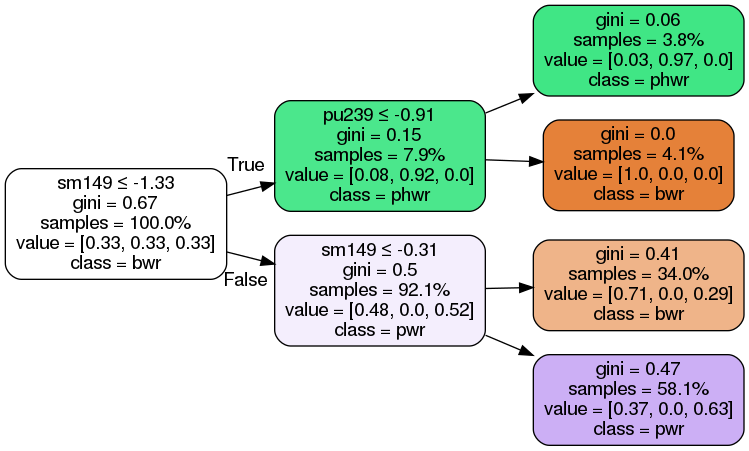
\includegraphics[width=\linewidth]{./chapters/litrev/dtree.png}
  \caption{Example of a decision tree process, where maximum tree depth was 
           limited to 2 for vizualization purposes.}
  \label{fig:dtr}
\end{figure}

In Figure \ref{fig:dtr}, the first split is determined to occur at the feature
Sm149 on whether the nuclide measurement is above a value of $-1.33$. Note that
this value is negative because of the scaling process the training set is put
through, described in Section \ref{sec:statmodel1}. The majority class at this
node is \gls{BWR} which is expected since the training set is 72\% \gls{BWR}.
The values list indicates the fraction of each class in the node, which is
alphabetically ordered \texttt{[bwr, phwr, pwr]}. It is even among the three
because the class weights were told to be balanced.  This splitting criterion
provides a Gini impurity score of 0.67, which represents the minimum Gini
impurity of all the candidate splits, but also indicates there are multiple
classes represented in this node (again, expected).  It would be 0 if there
were only one class in the node.  In the visualization, the shading of the
colors in the tree are bolder for there being a higher fraction of a single
class.

\subsubsection{Maximum Log-Likelihood Calculations}

The \gls{MLL} calulations approach applied here is based on a method developed
to do similar work \cite{mll_method, mll_validate, mll_sensitivity}.  That work
involved matching nuclear material samples based on some select measurements to
entries in a database of containing those measurements (see Section
\ref{sec:stats4nf}).  Each database entry also has a similar list of labels to
the labels being predicted in this work: reactor type, burnup, and time since
irradiation.

Interestingly, the \gls{MLL} calculations method works like \textit{k}-nearest
neighbors, where there is no model but a prediction according to the closest
match database entry.  There is one detail that differs, however. Whereas
\textit{k}-nearest neighbors minimizes distance/dissimilarity, this approach
instead maximizes similarity via a likelihood function. An "unknown" test
sample is compared against the training set using the likelihood calculation
between that sample and the training set entries.  The higher the likelihood,
the higher the probability that the database entry represents the sample. The
likelihood is in Equation \ref{eq:like}, whereas the log-likelihood is used
more often in practice, shown in Equation \ref{eq:loglike}.
\begin{equation}
  L(M|x_{test}) = \prod_i \frac{1}{\sigma_{i,train} \sqrt{2\pi}} \exp{\frac{-(x_{i,test} - x_{i,train})^2}{2 \sigma_{i,train}^2}}
  \label{eq:like}
\end{equation}
\begin{equation}
  ln(L(M|x_{test})) = \sum_i ln(\frac{1}{\sigma_{i,train} \sqrt{2\pi}}) - \frac{(x_{i,test} - x_{i,train})^2}{2 \sigma_{i,train}^2}
  \label{eq:loglike}
\end{equation}
The likelihood is a measure of the probability that a model $M$ produced the
measurements seen in the test sample, given by $L(M|x_{test})$.  In both
Equations \ref{eq:like} and \ref{eq:loglike}, $x$ refers to the set of
features, and $x_{i, test}$ and $x_{i,train}$ are the individual features for the
test sample and the training set entries, respectively. The uncertainty of the
measurement associated with each feature is represented by $\sigma_{i,train}$.



\subsection{Model Selection and Assessment}
\label{sec:selectass}
After a model is trained, the first step is model selection and assessment.
Selection is estimating model performance among a set of trained models using a
single validation set.  After one model is chosen, assessment takes place by
determining the prediction capability on new data via a previously unseen
testing set. Both selection and assessment can be done in a single step using
\textit{k}-fold cross-validation, which is described below.

\subsubsection{Sources of Error} 

In statistical learning, there are two sources of error that need to be
simultaneously minimized: bias and variance. Bias is caused by simplifications
in the model, so the error is caused by missed relationships in the data; an
underfit model is due to high bias.  Variance is caused by including random
noise in the model, so the error is caused by oversensitivity to that noise; an
overfit model is due to high variance. 

%%%%%%%%%%%%%%%%%%%%%%%%%%%%%%%%%%%%%%%%%%%%%%%%%%%%%%%%%%%%
%%%%%%%%%%%%%%%%%%%%%%%%%%%%%%%%%%%%%%%%%%%%%%%%%%%%%%%%%%%%
Include math or just reference it?
Talk about irreducible error too?
%%%%%%%%%%%%%%%%%%%%%%%%%%%%%%%%%%%%%%%%%%%%%%%%%%%%%%%%%%%%
%%%%%%%%%%%%%%%%%%%%%%%%%%%%%%%%%%%%%%%%%%%%%%%%%%%%%%%%%%%%

\begin{figure}[!htb]
  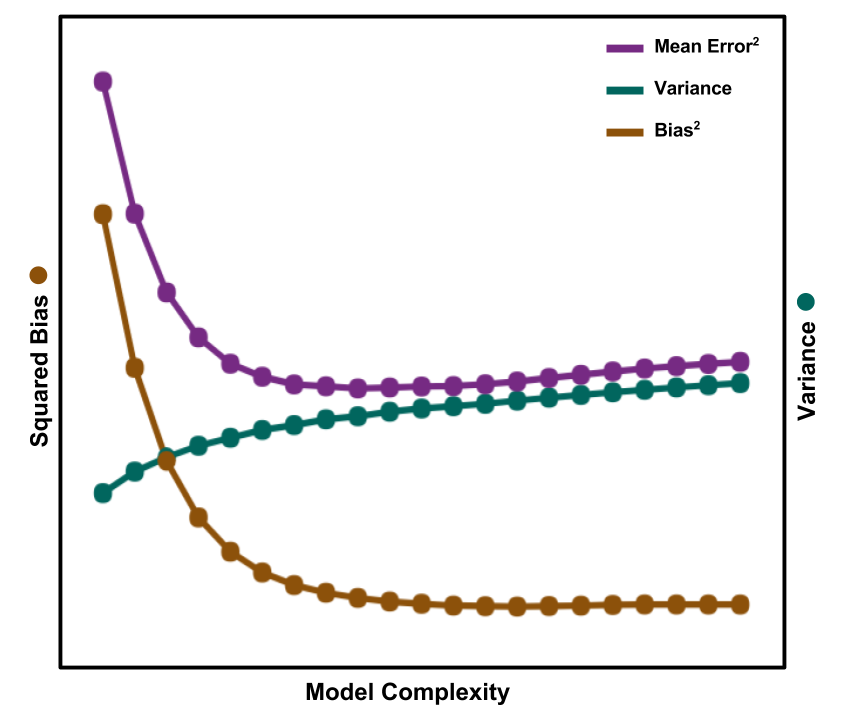
\includegraphics[width=\linewidth]{./chapters/litrev/BVtradeoff.png}
  \caption{Total prediction error comprised of bias and variance}
  \label{fig:bvtradeoff}
\end{figure}

As shown in Figure \ref{fig:bvtradeoff}, there is a minimum in the total error,
showing that there is a tradeoff between the bias and variance. Some bias is
desired in order to generalize to future unknown data. But some variance is
also positive for the model because it captures the relationships in the data
that the bias counteracts. 

\subsubsection{Types of Error}

While the sources of the model prediction error are well known, the creation of
a statistically learned model is a hidden process. Although the model emerges
from a black box, there are ways to evaluate the generalization (i.e.,
prediction) capability of it.  This is done by removing a small portion of the
data for use as a testing set.  The rest of the data set is known as the
training set and is used to train a model. After training, the test set is used
to test the model.  

The generalization error is typically referred to as the \textit{testing
error}, as it is measuring the ability of the model to predict future cases
that were not introduced in the training phase (i.e., the testing set entries).
Next, the \textit{training error} is provided by comparing the model
predictions to the training set, as the model would likely be smoother than the
potential noise the training set would include. This is useful to determine the
fitness of the model, the application of which is discussed below in Section
\ref{sec:optvalid}.

Although one could just train and test their model, there is a way to test the
model while still in the training phase. A testing set that would be used
during training to give feedback, a \textit{cross-validation} set, can provide
a faster convergence to a satisfactory model. As shown in Figure
\ref{fig:cverror}, this can be done by splitting the data set into three
groups: a large training set, a small cross-validation set, and a small testing
set. 

\begin{figure}[!htb]
  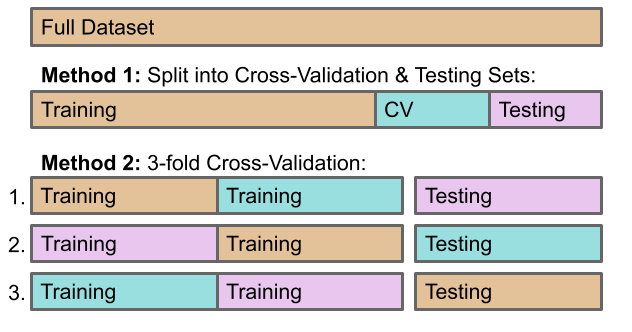
\includegraphics[width=\linewidth]{./chapters/litrev/cverror.png}
  \caption{Illustration of how a dataset can be split up for model evaluation}
  \label{fig:cverror}
\end{figure}

However, in practice, multiple rounds of cross-validation steps are used,
referred to as \textit{k-fold cross-validation}. This allows a user to use all
data entries as a testing entry once.  As illustrated in \ref{fig:cverror},
this splits the dataset into \textit{k} subsets. One set is designated as the
testing set, and a model is trained with the rest. Following the first training
phase, another begins, this time with a different subset as the testing set.
This process is performed \textit{k} times to give \textit{k} models, and the
models are then averaged, providing an additional level of model validation
than can be achieved with a single testing set.



\subsection{Model Optimization and Validation}
\label{sec:optvalid}
It is unlikely to have a model perform as one expects the first time. There are
therefore a few techniques for optimizing the performance. It should be noted
that much of the discussion here and in Section \ref{sec:valid} focuses on
the diagnostics aspect rather than the validation aspect of these techniques.
In practice, these are used for both purposes, but in this work the formal
comparison of model performance will be used, introduced and detailed in
Sections \ref{sec:invcompare} and \ref{sec:modelcompare}, respectively. 

However, the increase in performance from over-optimization could be linked to
the training set performance and might not generalize outside of the specific
type of input data used.  A workaround for this scenario is to obtain more data
for the set or to obtain a completely different data set altogether. 

\subsubsection{Training Set Size}

The first diagnostic plot for optimizing the model performance is called a
\textit{learning curve}, which provides information about the bias-variance
tradeoff with respect to the data set size. More specifically, learning curves
compare the training and cross-validation errors to the size of the training
set (i.e., number of instances in the training set). This is done by randomly
selecting a percentage of the the training set, inputting that into a
statistical learner, and tabulating the error of the learned model. 

Typically, a learning curve will look somewhat like one of the three examples
in Figure \ref{fig:learning}\footnote{These schematics are based on hand-drawn
diagrams by Ritchie Ng on http://www.ritchieng.com/applying-machine-learning/}.
A learning curve tests the model for high bias or high variance, which can
correspond to an undefit or overfit model, respectively. 

\begin{figure}[!hp]
  \centering
  \begin{subfigure}[h]{0.65\linewidth}
    \centering
    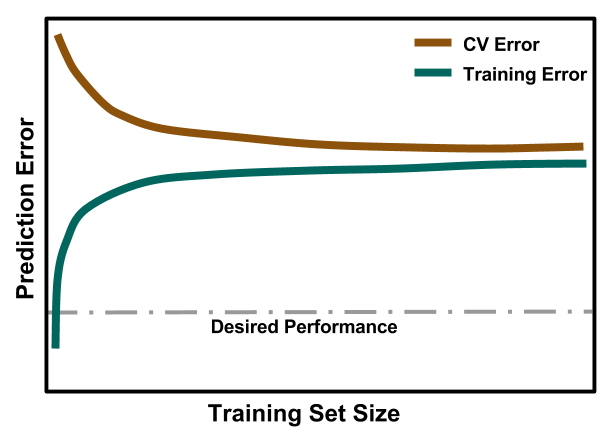
\includegraphics[width=\linewidth]{./chapters/litrev/LearningCurve-bias.png}
    \caption{High bias}
    \label{fig:bias}
  \end{subfigure}
  \begin{subfigure}[h]{0.65\linewidth}
    \centering
    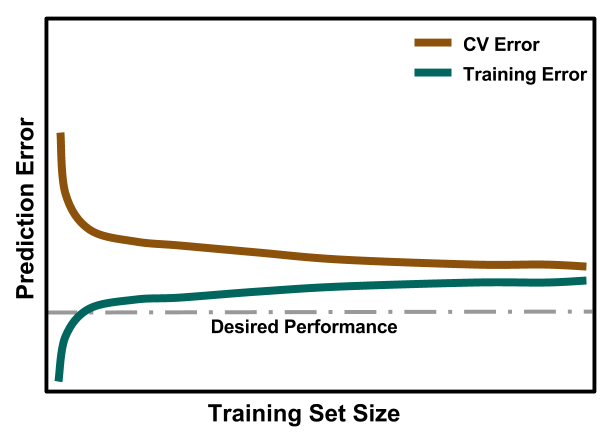
\includegraphics[width=\linewidth]{./chapters/litrev/LearningCurve-ideal.png}
    \caption{Ideal}
    \label{fig:ideal}
  \end{subfigure}
  \begin{subfigure}[h]{0.65\linewidth}
    \centering
    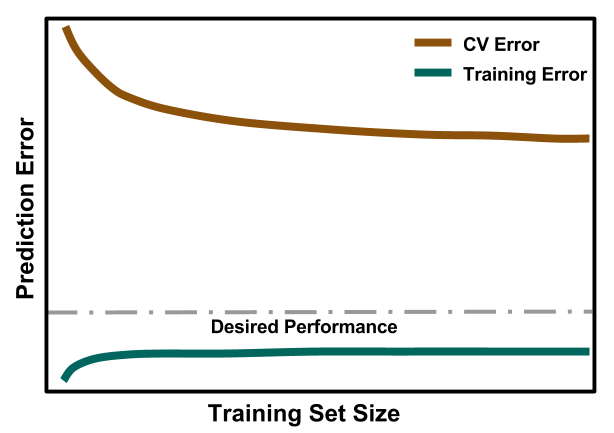
\includegraphics[width=\linewidth]{./chapters/litrev/LearningCurve-variance.png}
    \caption{High variance}
    \label{fig:variance}
  \end{subfigure}
  \caption{Learning curves for three training scenarios}
  \label{fig:learning}
\end{figure}

Figure \ref{fig:bias} suggests underfitting because the model is missing
important features in the data. It is characterized by a small gap between the
curves but high overall errors. The cross-validation error remains consistently
high and the training error increases drastically with increasing data, since
it is not generalizing well. 

Figure \ref{fig:variance} suggests overfitting because the model has too much
sensitivity to variations in the data. It is characterized by a very large gap
between the curves. It has an extremely low training error, as it has taken
into account every detail of the training set, but a high cross-validation
error because it cannot generalize beyond the testing set. 

Figure \ref{fig:ideal} is an example of a more ideal model fit. It is
characterized by a small gap between the two errors, and they are at a
reasonable level with respect to the desired performance.  The training error
should increase with respect to the training set size due to a larger amount of
bias (preventing overfitting). But the cross-validation error should decrease
quickly with respect to the training set size due to being close to the minimum
of the bias-variance tradeoff. 

\subsubsection{Model Complexity}

After ensuring the appropriate training set size is selected, the models must
be further optimized using \textit{validation curves}.  These provide
information on the bias-variance tradeoff with respect to model complexity. Two
main factors affecting model complexity can cause the model to be under- or
overfit to the data: number of features in the data set and algorithm
parameters that vary the regularization.

\begin{figure}[!htb]
  \centering
  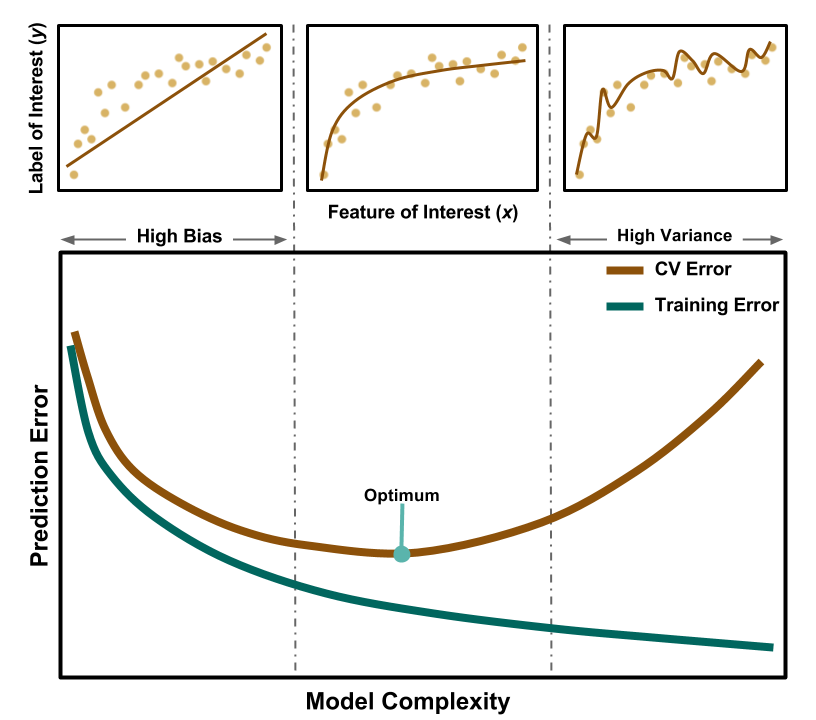
\includegraphics[width=1.05\linewidth]{./chapters/litrev/ValidationCurve.png}
  \caption{Validation curve showing examples of different fittings}
  \label{fig:validation}
\end{figure}

Figure \ref{fig:validation} adapted from Ref. \cite{elements_stats} shows the
optimum as the minimum of the cross-validation error curve. There is some gap
between it and the training error, much larger than the left side of the plot
and much smaller than the right.  The plot above is a visualization of a
decently fit model.  The left region is marked by both errors being quite high,
and above is an  illustration of how an underfit plot (high bias) could provide
high errors. The right region shows the training error being quite low but the
cross-validation error being high. The diagram above shows that it is obvious
how the training error would be negligible, but generalizing beyond that
probably will not yield accurate results. 

In practice, plotting learning and validation curves can be iterative. But as
previously mentioned, too many optimizations will result in a poorly performing
model when exposed to data outside of the training set.

\subsubsection{Comparison of Methods}
\label{sec:invcompare}

In addition to evaluating a single learned model, it will be beneficial to
compare models. This can be done using Bayesian inference as discussed in
Section \ref{sec:inverse}.  Equations \ref{eq:bayes} and \ref{eq:bayes_words}
show that there are three values to obtain to calculate a posterior
probability, i.e., the probability of a parameter estimated from a
machine-learned model being correct: the likelihood, the prior probability, and
the marginal likelihood. 

The posterior probability represents the solution to an \textit{inverse}
problem, where model parameters are predicted from some given measurement
values. It is not directly computable and thus the remaining probabilities
discussed below indirectly allow its computation.  In this context, it is the
probability that a predicted reactor parameter from a chosen method is correct
given input based on an \gls{SNF} recipe.  For example, it is the probability
that a plutonium-239 concentration of $y\%$ is attributed to a uranium oxide
fuel in a \gls{BWR} with a burnup of $x\ GWd/MTU$.  Most inverse problems are
\textit{ill-posed}, usually because the solution is not guaranteed to be
unique. The posterior probabilities compared across methods will provide the
most probable correct answer. This will reveal the superior method versus
others that have lower posterior probabilities. \cite{inverse_theory}

The likelihood represents the solution to a \textit{forward} problem, where
measurement values are predicted from some given model parameters.  In this
context, this is calculated from the instances in the training data set.  The
likelihood is the probability that the output \gls{SNF} composition of a
simulation is correct given the input of reactor operation parameters.  In
practice, it will be calculated from a large number of forward simulations
using \gls{ORIGEN}, i.e., the training data set. For example, this would be the
probability that uranium oxide fuel from a \gls{BWR} having a burnup of $x\
GWd/MTU$ contains $y\%$ of plutonium-239.

The prior probability represents the spread of plausible model parameters, so
it is a hypothesis based on the breadth of the model space with no evidence
provided.  In other words, it is given by model parametertization from a number
of potential sources.  One method is expert-elicited values. Another is a
predicted model from some established theory or previously known relationship,
e.g., empirical relations between isotopic ratios and certain reactor
parameters or a direct calculation of the reactor parameters. In this context,
it is obtained from the estimated model parameters from a given statistical
model.  For example, it is the probability that a model from \gls{SVR} predicts
a burnup of $x\ GWd/MTU$ for uranium oxide fuel from a \gls{BWR} with no other 
direct measurements provided.

The marginal likelihood represents the spread of plausible measurements, so it
is based on the breath of the data space with no model-based information
provided.  In practice, however, it is calculated by summing the joint
probabilities of all possible model parameter hypotheses and measurements. This
in essence provides a normalization constant.  Thus, the marginal likelihood is
only needed for absolute posterior probability calculations; it does not affect
the relative probabilities, which are all that is needed for model comparison
\cite{inverse_theory}. 

For reference, Table \ref{tbl:bayes} is a summary of the Bayes' theorem
components described above as related to this work.

\begin{table}[!hp]
  \centering
  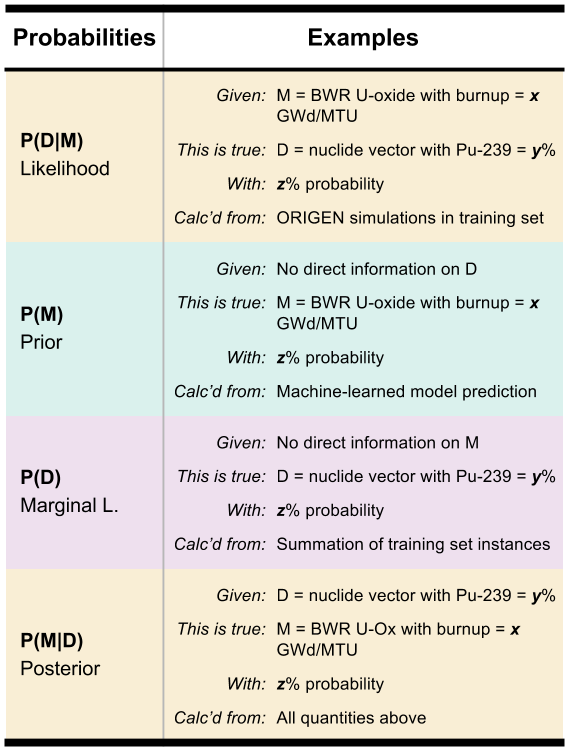
\includegraphics[width=\linewidth]{./chapters/litrev/bayes.png}
  \caption{Summary of contextual explanations of Bayes theorem components}
  \label{tbl:bayes}
\end{table}




\section{Computational Methods}
\label{sec:fcsim}
There can be a large number of computational tools within a given field of
study.  They are typically developed with one aspect of analysis in mind, so
one must understand the simplifying assumptions the developers made for their
purposes. Thus, choosing a computational tool is not always obvious. Thus, this
section both introduces and defends the choices for the various experimental
components.

\subsection{Fuel Cycle Simulation}

Nuclear fuel cycle studies involve tracking the material flow of nuclear fuel.
This can be anywhere from mining to waste management, or focus on a process
step anywhere in between. Fuel cycle studies are not necessarily
nuclear-specific. They can be used to evaluate, e.g., economic predictions,
environmental impact, transportation planning, etc.  In order to draw
conclusions from these studies, it is common to use a nuclear fuel cycle
simulator that tracks the quantities of interest. These allow the comparison of
different fuel types, reactor technologies, material processing steps, etc. 

As mentioned, there are simplifications researchers need to make in order to
experiment in a controlled way. Fuel cycle simulators are built for specific
needs as well and also must remove complicating factors that are generally less
relevant to the study.  For example, one tool might be suited well to
large-scale systems analysis with little nuclear physics included in the
models, and another might focus on detailed isotopics within a system to track
plutonium isotopes.

\todo{more needed?}

Because a large portion of a nuclear forensics investigation relies on
measuring isotopics, \gls{ORIGEN-ARP} \cite{origen} within the SCALE code
system was chosen for its physically detailed models. \gls{ORIGEN} calculates
time-dependent nuclide concentrations (or quantities derived from these) that
result from activation and depletion calculations. The physics (i.e., neutron
transport and decay) calculations are carried out in other SCALE modules that
solve the depletion equations.  This generates libraries for \gls{ORIGEN} that
include the probabilities of reaction (i.e., cross sections) for the system.

To obtain an \gls{SNF} recipe from a reactor simulation, \gls{ORIGEN} uses the
desired input power generation with the cross section library to calculate a
flux, the resulting depletion, and the end composition (i.e., isotopics,
nuclide vector).  Another output is decay; the composition is computed using
decay equations with nuclear data \cite{endf}. These compositions provide
source terms for other calculations, such as decay emission spectra from
neutrons, or alpha, beta, gamma rays, which use the same resource for nuclear
data. Other quantities like activity, decay heat, or radiological hazard
factors are also an option.

\gls{ORIGEN-ARP} allows users to access a wider range of simulations by
interpolating between the already calculated libraries for a wide array of
reactors instead of creating new libraries.  It is known to be validated for
\gls{LWR} \gls{SNF} \cite{lwr_valid}. Additionally, recycled \gls{SNF} in the
form of mixed oxide fuel has been benchmarked with the relevant reactors
\cite{mox_valid}.  Thus, given an initial material composition, some reactor
operation parameters, and a reactor type, one can quickly perform many
different nuclear reactor simulations and obtain \gls{SNF} recipes.

\subsection{Statistics Toolkit}

The statistics toolkit chosen for this work is scikit-learn \cite{scikit}, a
machine learning package in python.  Virtually all modern machine learning
toolkits will have acceptably fast and reliable algorithms, but the use of
python provides a platform for seamless integration of all the tools in the
workflow. 

\subsection{Computational Gamma Spectra}

Although the data modification shown later in Section \ref{sec:inforeduc} does
not use any standalone tool, the code \gls{GADRAS} \cite{gadras} developed at
Sandia National Laboratories will provide information reduction in a physically
valid manner.  Test studies will be carried out using the gamma spectra
available from \gls{ORIGEN} simulations, but the detector response will need to
be varied more than this tool can provide. Thus, given the nuclide vectors from
\gls{ORIGEN}, \gls{GADRAS} computationally generates gamma spectra from the
gamma energies and a chosen \gls{DRF}. This will enable a more robust study of 
statistical performance with respect to information reduction.



\section{Applications of Statistical Methods to Nuclear Forensics Analysis}
\label{sec:stats4nf}
I'm the lit review section on previous applied ML work in the NF field.

\subsection{Special Nuclear Materials Studied}

The review on nf for the whole fuel cycle is useful here, perhaps. This is also 
important when I discuss my risk management section later. 

\subsection{Statistical Methods Employed}

Very short details from lit review outline and success rates should be 
discussed here




\glsresetall

\chapter{Reactor Parameter Prediction Using Nuclide Masses}
\label{ch:exp1}

This chapter covers the parameter prediction workflow using nuclide masses as
the input features. The methodology is introduced by detailing each
experimental component and its implementation. This is split into four
sections, which correspond to the four steps summarized in Figure
\ref{fig:method}.

\begin{figure}[!ht]
  \centering
  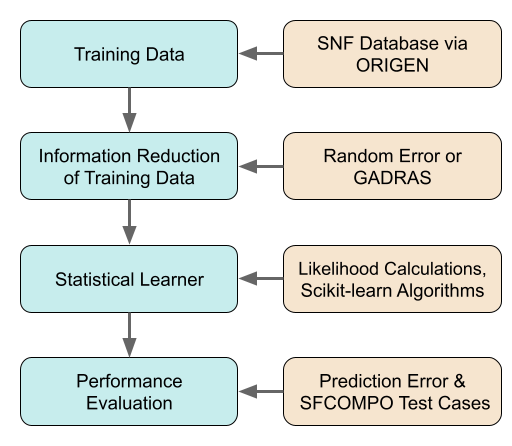
\includegraphics[width=0.7\linewidth]{./chapters/exp1/methodology.png}
  \caption{Flowchart of the experimental methodology and the way each step is being implemented.}
  \label{fig:method}
\end{figure}

Section \ref{sec:training1} discusses how the training data set is obtained
through simulations and computational means. The initial training data
simulated via \gls{ORIGEN} is detailed in Section \ref{sec:training1} This
provides a set of \gls{SNF} observations with known reactor operation
parameters, i.e., labels that are to be predicted. The four labels being
predicted are as follows:
\begin{enumerate}
  \item The classification of the \textbf{reactor type} is one of the three
        most common commercial power reactors: \gls{PWR}, \gls{BWR}, or 
        \gls{PHWR}.
  \item The \textbf{burnup} describes how much energy was produced by the fuel
        and has the units : $MWd/MTU$ or $GWd/MTU$, \textit{mega (or giga) 
        watt-days per metric ton of initial uranium}.
  \item The \textbf{enrichment} is the percentage of \gls{U235} with respect to
        the entire amount of uranium in the fuel: $\%U235$. 
  \item Lastly, the \textbf{time since irradiation}, or cooling time, is
        defined as how long the fuel has been out of the reactor core: $days$ 
        or $years$.
\end{enumerate}

Next, the information reduction step is covered in Section
\ref{sec:inforeduc1}, where uniform error is randomly applied. After this, the
less-precise training data sets will be input to a statistical learner for the
next step: training models.

Section \ref{sec:statmodel1} details the implementation of the algorithms
introduced in \ref{sec:algs}. They use the features and labels in the training
data sets to formulate a model. 

After this, the algorithms must be evaluated for their prediction performance
when given test samples (i.e., a new \gls{SNF} measurement that has no labels
according the to algorithm).  The approach is shown in Section \ref{sec:eval1}.
First presented is the prediction performance of samples that are taken out of
the training data set to be used as test cases, which is shown in Section
\ref{sec:randerr}.  Second, an external test set with nuclide concentrations is
used to show how this approach performs with real world measurements. This is
discussed in Section \ref{sec:sfcompo}.  

\section{Training Data Simulation}
\label{sec:training1}
\begin{figure}[H]
  \centering
  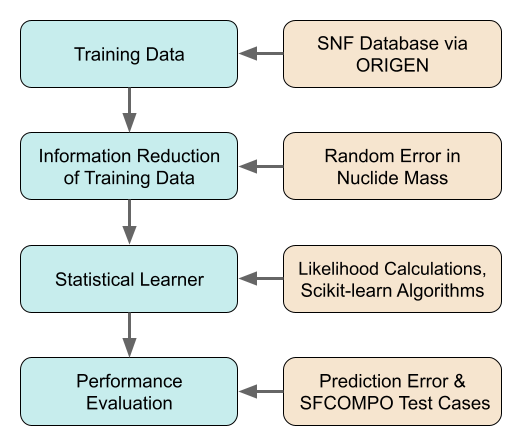
\includegraphics[width=0.7\linewidth]{./chapters/exp1/methodology1.png}
  \caption{First portion of the flowchart from Figure \ref{fig:method} being 
           described in this section.}
\end{figure}

Of interest to an entity trying to create a weapon is partially irradiated fuel
if they have plutonium separations capabilities or any radioactive substance in
the case of a dirty bomb. Thus, this work focuses on \gls{SNF} from commercial
power reactors. Ideally, a large enough database of \gls{SNF} nuclide assays
would be able to be used for this work. Since that does not exist, the 
database will be simulated via \gls{ORIGEN-ARP} \cite{origen, origenarp}.  

\subsection{Simulation Fidelity}
\label{sec:fidelity}

Nuclear fuel cycle studies involve tracking the material flow of nuclear fuel.
This can be anywhere from mining to waste management, or focus on a process
step in between. Fuel cycle studies are not necessarily nuclear-specific. For
example, they can be used to evaluate economic predictions, environmental
impact, transportation planning, etc.  In order to draw conclusions from these
studies, it is common to use a nuclear fuel cycle simulator that tracks the
quantities of interest. These allow the comparison of different fuel types,
reactor technologies, material processing steps, etc. 

There are simplifications researchers need to make in order to experiment in a
controlled way. Fuel cycle simulators, built for a specific needs, must remove
complicating factors that are less relevant to the study.  For example, one
tool might be suited well to large-scale systems analysis with little nuclear
physics included in the models, and another might focus on detailed isotopics
within a system to track plutonium.

Because a large portion of a nuclear forensics investigation relies on
measuring isotopics, this work used \gls{ORIGEN} \cite{origen}, which is a part
of the \gls{SCALE} 6.2 modeling and simulation suite of computational tools
developed for nuclear design and safety \cite{scale}. \gls{ORIGEN} was chosen
for its physically detailed models of activation, depletion, and decay.
Specifically, the ARP module of the code was used: \gls{ORIGEN-ARP}
\cite{origenarp}.

\gls{ORIGEN} calculates time-dependent nuclide concentrations (or quantities
derived from these) that result from activation and depletion calculations. The
physics (i.e., neutron transport and decay) calculations are carried out in
other \gls{SCALE} modules that solve the depletion equations.  This generates
libraries for \gls{ORIGEN} that include the probabilities of reaction (i.e.,
cross sections) for the system.

To obtain an \gls{SNF} recipe from a reactor simulation, \gls{ORIGEN} uses the
desired input power generation with the cross section library to calculate a
flux, the resulting depletion, and the end composition (i.e., isotopic recipes
or nuclide vectors).  Another output is decay; the composition is computed
using decay equations with nuclear data \cite{endf}. These compositions provide
source terms for other calculations, such as decay emission spectra from
neutrons, alpha particles, beta particles, and gamma rays. Other derived
quantities like activity, decay heat, or radiological hazard factors are also
an option.

\gls{ORIGEN-ARP} allows users to access a wider range of simulations by
interpolating between the pre-calculated libraries instead of creating new
libraries.  It is known to be validated for \gls{LWR} \gls{SNF}
\cite{lwr_valid}. Additionally, recycled \gls{SNF} in the form of mixed oxide
fuel has been benchmarked for the relevant reactors \cite{mox_valid}.  Through
\gls{ORIGEN}, given an initial material composition, some reactor operation
parameters, and a reactor type, one can quickly perform many different nuclear
reactor simulations and obtain \gls{SNF} recipes.

\todo[inline]{This section needs more information about ORIGEN-ARP validation
and maybe some nuclides that are known to perform poorly from ARP sims. Can
show a generic example from one of my sources, and or an example of trying to
match an ORIGEN-ARP simulation to an SFCOMPO entry. It is important to inform
that this training set as ground truth is not perfect truth, for some nuclides
more than others. The goal is to explain the ARP validation without getting
too deep.  This tool was necessary for the 500k training set. The prediction
performance will be impacted by the poorly simulated nucs, so it may be
worthwhile to note which ones have consistently large sim errors (unless this
involves getting too deep). P.S. did you mention homogenized core above?}

\subsection{Training Set Labels}
\label{sec:snflbls}

\begin{table}[!htb]
  \centering
  \begin{subtable}{\linewidth}
    \centering
    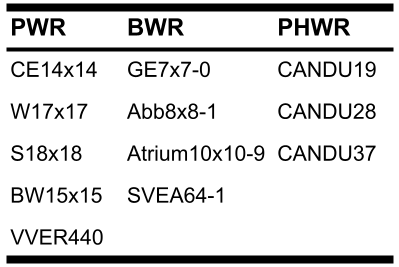
\includegraphics[width=0.5\linewidth]{./chapters/exp1/trainset4_Orxtrs.png}
    \caption{\gls{ORIGEN} designations for reactor technologies and fuel assembly design.}
    \label{tbl:rxtrtype}
    \vspace*{5mm}
  \end{subtable}
  \begin{subtable}{\linewidth}
    \centering
    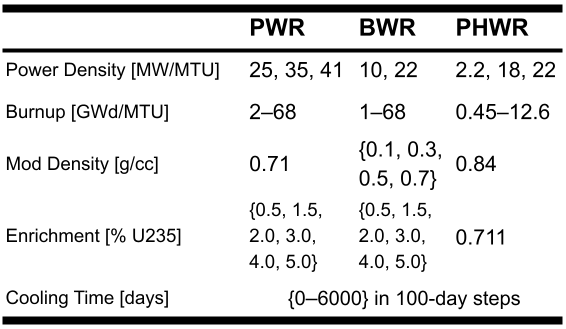
\includegraphics[width=0.75\linewidth]{./chapters/exp1/trainset4_inputs.png}
    \caption{Simulation parameters for \gls{ORIGEN} input files.}
    \label{tbl:rxtrparam}
  \end{subtable}%
  \caption{Training set database design using the \gls{SFCOMPO} database as guidance. \cite{sfcompo}}
  \label{tbl:train}
\end{table}

The design of the training set is dependent on a number of factors.  First, it
must have a sufficient number of burnup sets and time since irradiation steps
to provide robust prediction. This is decided upon by maximizing the steps for
both parameters, while balancing the computational limitations of a large
training set. Through previous experience, an approximate limit would be around
$1e6$ database entries for the specific calculations in this work and employing
reasonable computational limitations.

Secondly, the training set must represent what exists in the real world. This
was accomplished by studying the spread of parameters in the \gls{SFCOMPO}
database \cite{sfcompo}.  To ensure this, a variety of reactor types and
assembly designs were included, listed in Table \ref{tbl:rxtrtype}. Table
\ref{tbl:rxtrparam} lists the rest of the simulation inputs. These include not
only the labels of prediction interest, \gls{U235} enrichment, burnup, and time
since irradiation, but also other important simulation input parameters such as
the reactor power density and the moderator density.  (Water is both the
moderator and coolant in all simulated reactor types.)

\begin{figure}[!hbt]
  \makebox[\textwidth][c]{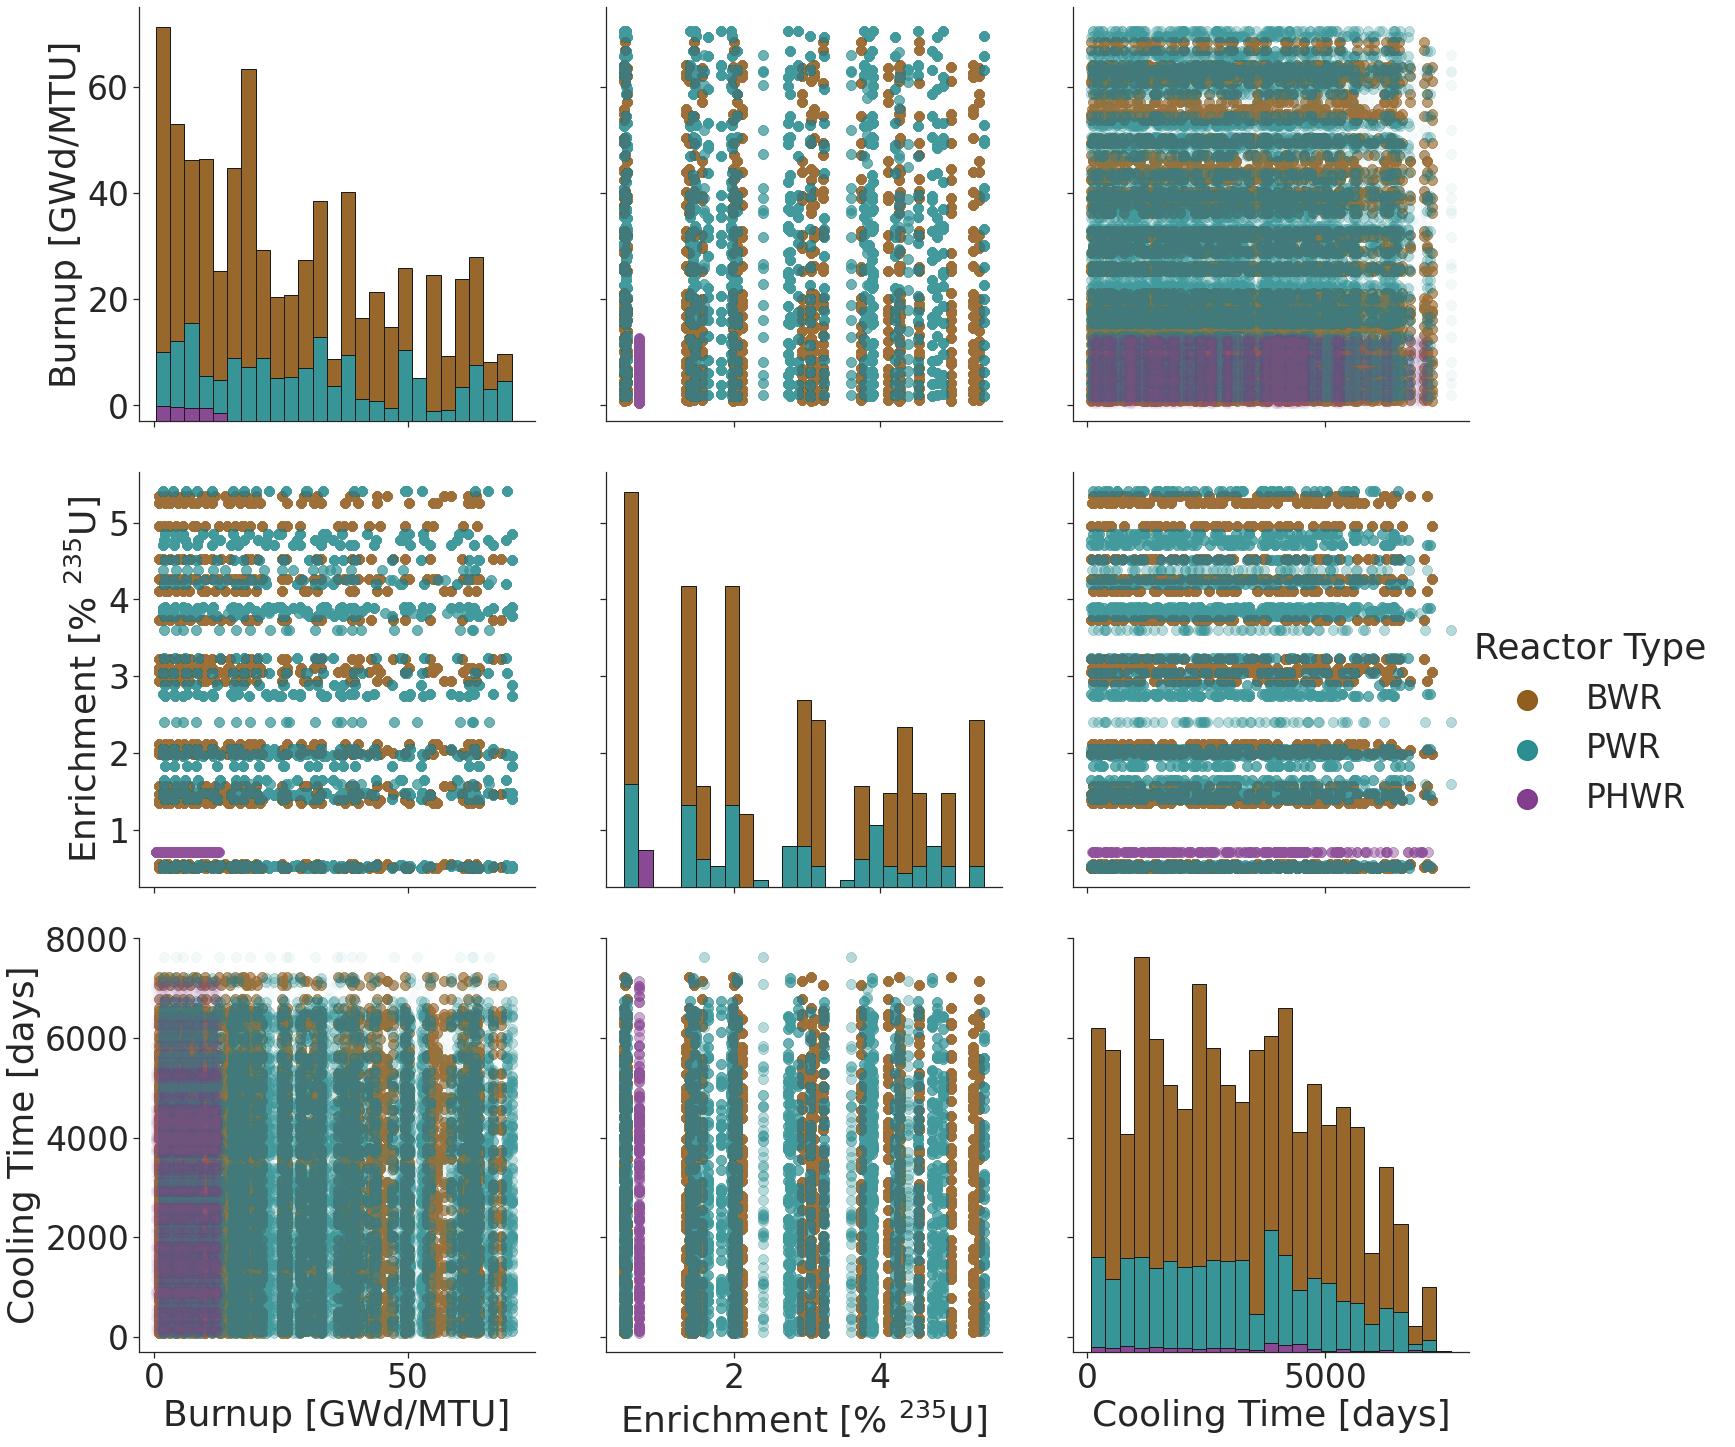
\includegraphics[width=\linewidth]{./chapters/exp1/histogram_scatter_trainset_viz.png}}
  \caption{A combination of histograms and scatter plots to visualize the 
           distribution of prediction labels in the training set.}
  \label{fig:trainhist}
  \todo[inline]{fix the histogram figure, this is a placeholder}
\end{figure}

The third factor influencing database design is ensuring ideal \gls{ML}
algorithm performance.  As mentioned in Section \ref{sec:errs}, many algorithms
are developed with the assumption that the training set will be
\acrfull{i.i.d.}.  This is important so that the model does not overvalue or
overfit a certain area in the training space. With the training set design,
there are predetermined values for enrichment, burnup, and time since
irradiation.  While there are $21-28$ burnup steps (depending on the reactor
type) and 61 cooling time steps, there are only 6 values for enrichment. This
creates the risk that the algorithm will end up being unable to generalize
outside of those discrete values. Therefore, the burnup steps and time steps
are perturbed randomly in a range that is $\pm10\%$ and $\pm30\%$ from the
originally defined values, respectively.  The enrichment also gets perturbed by
$\pm10\%$, and not more because the cross-section libraries in \gls{ORIGEN-ARP}
are pre-calculated for those enrichment values, so deviating too far from them
would result in inaccurate \gls{SNF} simulations. The power densities and
moderator densities were kept at the values defined in Table
\ref{tbl:rxtrparam}.  The resulting training set is $450240$ (or $4.5e5$)
entries.  Figure \ref{fig:trainhist} visualizes the somewhat even distribution
of the burnup and cooling time parameters, and shows the lack of even
distribution of the enrichment parameter through a combination of scatter plots
and histograms.  Note that there are many more \gls{BWR}s present in the
histograms because of the multiple moderator densities simulated (see Table
\ref{tbl:rxtrparam})

\subsection{Training Set Features}
\label{sec:snffeats}

The other design decision regarding the training set is related to
which nuclides to track, i.e., the features.  For this experiment, nuclide
masses are necessary, and the most common measurements in \gls{SFCOMPO} guide
the list of nuclides tracked.  

The set of training features of 29 nuclide masses listed in Table
\ref{tbl:nucmass} was designed with the following reasons in mind.  First, the
units in mass is to represent the scenario of "perfect knowledge", where a full
assay is done via mass spectrometry techniques.  Second, this is to have the
training set units convertable to those present in the external, real-world
test set: the \gls{SFCOMPO} database.  The \gls{ORIGEN} simulations output the
nuclide masses in $grams$, and they are converted to the units of
\textit{milligrams per gram of initial uranium}, $mg/gU_i$, when the models are
externally tested against \gls{SFCOMPO}. Lastly, the 29 nuclides chosen were
based on the presence of measurements in \gls{SFCOMPO}, where these were
present in at least 100 of the samples in the database.  The external test set
is described in more detail in Section \ref{sec:sfcompo}.

\begin{table}[!htb]
  \centering
  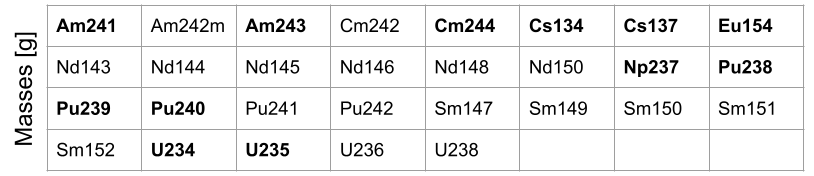
\includegraphics[width=\linewidth]{./chapters/exp1/nucmass_feats.png}
  \caption{Set of features saved for the first experiment, nuclide masses 
           measured in $grams$. The bold nuclide masses overlap with the 
           nuclides in \ref{tbl:nucacts}.}
  \label{tbl:nucmass}
\end{table}



\section{Information Reduction}
\label{sec:inforeduc1}

\begin{figure}[H]
  \centering
  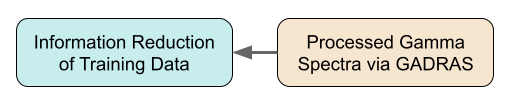
\includegraphics[width=0.7\linewidth]{./chapters/exp2/methodology2_2.png}
  \caption[Second portion of the flowchart from Figure \ref{fig:method2}]
          {Second portion of the flowchart from Figure \ref{fig:method2} being 
           described in this section.}
\end{figure}

The overall goal of this project is to determine how much information to what
quality is needed to train a  \gls{ML} model that can provide \gls{SNF}
attribution by correctly predicting the reactor type, burnup, \gls{U235}
enrichment, and time since irradiation.  In this section, the information
quality is treated as the energy resolution of gamma spectra from several
detectors.  This is because field-deployable detectors are of interest.

This process is outlined here for the second experiment, in which a gamma
spectrum is computed for each sample in the database from the nuclide
activities in Section \ref{sec:training2}.  The \gls{GADRAS} code \cite{gadras}
developed at Sandia National Laboratories will provide computational gamma
spectra. There are four steps to this process: choosing radionuclides,
inputting the radionuclide activities into a \gls{DRF} to compute gamma
spectra, processing the gamma spectra into a smaller feature set, and applying
a statistical counting error to those features.

\noindent \textbf{Step 1: Choosing Radionuclides}

The first step of is covered in Section \ref{sec:training2}.  

\noindent \textbf{Step 2: Computational Gamma Detection}

The second step is obtaining a gamma spectrum for every \gls{SNF} entry in the
database; this is done using \gls{GADRAS}. The \gls{GADRAS} tool includes many
capabilities related to radiation detection and spectra analysis; its
predominant use is related to the simulation of the detection of gamma rays and
neutrons from user-defined sources and detector configurations.  A combined
first principles and empirical modeling approach based on interaction cross
sections and radiation scattering inform the \glspl{DRF} code to calculate
typical gamma detector spectrum features, e.g., photopeaks and the Compton
continuum.  Although new detectors can be created and calibrated within the
software, this work employs the use of pre-calibrated detectors.  Thus, given a
source, which is a list of radionuclides and their activities in this case,
\gls{GADRAS} applies a \gls{DRF} from a given detector configuration to the
gamma energy lines from these radionuclides and models the spectrum.
\cite{gadras} 

The nuclide activity data requires some processing to be used in this way.  The
activities that come from the \gls{ORIGEN} simulations are based on there being
$1\:MT$ of initial uranium-based fuel. Not only is this quantity an unlikely
amount to be smuggled, it would overwhelm a detector at the calibrated
source-detector distances in \gls{GADRAS}.  Therefore, the material (and
resulting nuclide activities) are scaled to be $1\:g$ of \gls{SNF}.

For the \gls{GADRAS} calculations, the primary input is a nuclide activity
vector as the source, and the output is an array of energy bins (measured in
$keV$) and the counts per energy bin as the spectrum.  The sources are provided
without any background; this is because any spectrum would undergo background
subtraction before further analysis. Additionally, the nuclides are pre-decayed
in \gls{ORIGEN} to correspond to various cooling times, but a source age must
be provided to \gls{GADRAS} as a non-zero value (otherwise, important decay
transitions are missed). Various source times ($10\:sec$, $30\:sec$, $1\:min$,
$5\:min$, $10\:min$, $20\:min$, $30\:min$, $1\:hr$, $2\:hr$) were tested for
two samples, and both a qualitative visual analysis of the major photopeaks
plus a study of the total counts leveling off was used to choose a nonzero age
for the material.  At a source age of $20\:minutes$, the expected peaks are
visible and the total counts had reached a value similar to the longer ages
tested.

The other input information is related to the detector configuration.
User-chosen variables are the source-detector distance $[cm]$, height of
source-detector setup from nearest surface $[cm]$, the live time $[s]$, and the
number of channels for the detector. The detector configuration file in
\gls{GADRAS} contains much more information, however.  In it, there are a
number of parameters from calibration results, detector geometry, information
about scattering, and shielding information (shielding is not considered in
this work).

\begin{table}[!htb]
  \centering
  \begin{tabular}{@{}lcllll@{}}
  \toprule
    \textbf{Detector} &
    \textbf{\begin{tabular}[c]{@{}c@{}}\% FWHM \\ @ 661 keV\end{tabular}} &
    \textbf{\begin{tabular}[c]{@{}l@{}}Distance \\ (cm)\end{tabular}} &
    \textbf{\begin{tabular}[c]{@{}l@{}}Height \\ (cm)\end{tabular}} &
    \textbf{\begin{tabular}[c]{@{}l@{}}Live Time\\ (s)\end{tabular}} &
    \textbf{\begin{tabular}[c]{@{}l@{}}Num \\ Channels\end{tabular}} \\ \midrule
    In-Lab HPGe           & 0.21 & 100.0 & 84.0  & 600  & 8192 \\
    Portable HPGe         & 0.29 & 100.0 & 100.0 & 600  & 8192 \\
    CZT                   & 1.20 & 100.0 & 100.0 & 600  & 1024 \\
    SrI\textsubscript{2}  & 2.94 & 100.0 & 100.0 & 600  & 1024 \\
    LaBr\textsubscript{3} & 3.63 & 213.0 & 84.5  & 2400 & 1024 \\
    NaI                   & 7.74 & 213.0 & 85.4  & 2400 & 1024 \\ \bottomrule
  \end{tabular}
  \caption[Details of detector setups]
          {Select details of 6 detector setups used to obtain gamma 
           spectra-based training databases.}
  \label{tbl:detsetups}
\end{table}

Training databases were created for the six detectors outlined in Table
\ref{tbl:detsetups}. They were chosen to compare the highest energy resolution
detector, a lab-based \gls{HPGe}, against the rest, in order of decreasing
energy resolution: portable \gls{HPGe}, \gls{CZT}, \gls{SrI2}, \gls{LaBr3}, and
\gls{NaI} detectors. This is displayed in the table by including the \gls{FWHM}
of the $661\:keV$ peak for ${}^{137}\text{Cs}$. \Gls{GADRAS} is used to create
a spectrum for every \gls{SNF} entry in the 32 nuclide activity training
database using these six detector configurations.  At this point, there are six
versions of the original database, one for each detector.  The database entries
are each a full gamma spectrum of a given \gls{SNF} sample for the detector
setup in that training set. 

\noindent \textbf{Step 3: Processing Gamma Spectra}

The third step covers the processing of the gamma spectrum generated for each
\gls{SNF} entry into a training set.  It is not computationally prudent to use
full gamma spectra for training and testing, since the spectra returned have
1024 or 8192 bins, and machine learning algorithms are not designed to handle
thousands of features.  Thus, these spectra are processed into fewer features; 
this is outlined as follows.

There is much ongoing work on the topic of attributing \gls{SNF} with gamma
detection using targeted or advanced measurement techniques \cite{snf_gamma,
compton_supp, bwr_high-res_gamma, pwr_bwr_gamma} and using innovative spectra
evaluation and radioisotope identification methods \cite{riid_09,
rapid_riid_18, sull_gen_07, sull_valid_15, sull_auto_17, sull_unc_17}.  \todo{update citations} Since
this is a topic of active research and the approaches are heavily
detector-dependent, a simple processing approach is developed here.  Since all
entries in a given training set are background-subtracted spectra using the
same detector setup and calibration for the same measurement duration, each
photopeak can be directly compared to other photopeaks in the training set.
This is accomplished by comparing them via an area under the curve: placing an
energy window on a peak, and summing the counts of the bins within that energy
window. 

There are two main design choices here: the width of the energy windows and the
number of energy windows to include. First, the energy window width is a value
that is fixed for each detector prior to processing.  The different energy
window widths are listed in Table \ref{tbl:enwindows}.  They are chosen
manually; the spectra were plotted and different values were tested and
visually analyzed to be sure the windows were encompassing the peaks. This was
preferable to some linear function based on the detector energy resolution
because, e.g., the \gls{LaBr3} and \gls{NaI} detectors have the same
human-chosen window but the energy resolutions are different (see Table
\ref{tbl:detsetups}). 

\begin{table}[!htb]
  \centering
  \begin{tabular}{@{}lcm{0.7in}m{0.7in}m{0.7in}@{}}
    \toprule
    \multirow{2}{*}{\textbf{Detector}} &
    \multirow{2}{*}{\textbf{\begin{tabular}[c]{@{}l@{}}Energy Window\\ Size {[keV]}\end{tabular}}} &
    \multicolumn{3}{c}{\textbf{\# of Energy Windows}} \\ \cmidrule(l){3-5}
                     &    & Auto & Short & Long \\
    \toprule
    In-Lab HPGe      & 2  & 206  & 42    & 151  \\
    Portable HPGe    & 3  & 120  & 42    & 151  \\
    CZT              & 8  & 30   & 42    & 151  \\
    $\text{SrI}_2$   & 10 & 17   & 42    & 151  \\
    $\text{LaBr}_3$  & 12 & 19   & 42    & 151  \\
    NaI              & 12 & 9    & 42    & 151  \\ 
    \bottomrule
  \end{tabular}
  \caption[Energy window sizes and list lengths for processing gamma spectra]
          {Energy window sizes and list lengths for 6 detector setups used to 
           process the gamma spectra-based training databases.}
  \label{tbl:enwindows}
\end{table}

The second design decision is the number of energy windows to include.  Table
\ref{tbl:enwindows} lists three energy window list length columns,
\textit{Auto}, \textit{Short}, and \textit{Long}. These correspond to different
processed training sets that have a different number of energy windows
included.  There are two approaches taken: a nuclear physics-based method that
generates an energy window list based on the gamma energies expected to be
detected (short and long), and an automatic peak search of a manually chosen
gamma spectrum in the full gamma spectra training database (auto). 

The first energy window list method provides the short and long lists in Table
\ref{tbl:enwindows}; the length of these lists are the same for all detectors
because they are based on the gamma energies most likely to be detected, which
is independent of the detector quality. To obtain these lists, the expected
number of decays of each gamma energy is calculated based on the activities of
the 32 tracked nuclides using the Python for Nuclear Engineering toolkit
\cite{pyne} from a reference sample in the training set.  This reference sample
emerged as the sample of choice because it contains the superset of gamma
energies of all tested samples, of which there were nine (three for each
reactor type).

After the expected number of decays for each gamma energy for all 32 nuclides
are calculated, an arbitrary minimum number of decays is selected to filter out
the gamma energies that are unlikely to produce counts high enough to be
detected. The first arbitrary minimum number of decays is set at $5 \times
10^8$ decays, and the long list of 151 gamma energies that remain above this
cutoff is created.  A list of length 151 is likely to contain many features
that do not contribute discrimination to the models, and thus they may add
noise to the training set, so a shorter list is needed.  So, a higher arbitrary
minimum of $5 \times 10^{10}$ decays is chosen; this threshold creates the
short list of 42 gamma energies. 

The short and long lists of gamma energies correspond to the nuclides in Table
\ref{tbl:enlistnucs}. The 12 nuclides listed come from the long list, and the
subset of seven bold nuclides come from the short list.  To determine a "full
knowledge" scenario for the detector-based training sets, two training sets are
also created with the 7- and 12-nuclide activity lists.  It should be noted
that several (three for each reactor type) training set entries were selected
based on sampling evenly throughout the training set parameters, with the
intention that there would be a set of gamma energies comprised from multiple
entries. However, one sample emerged as a superset of the others. This sample
is thus chosen for the second method, discussed next.

\begin{table}[!htb]
  \centering
  \begin{tabular}{@{}|l|l|l|@{}}
    \hline
    \allbold{${}^{241}\text{Am}$} & \allbold{${}^{243}\text{Am}$} & ${}^{243}\text{Cm}$           \\ \hline
    ${}^{244}\text{Cm}$           & ${}^{245}\text{Cm}$           & \allbold{${}^{134}\text{Cs}$} \\ \hline
    \allbold{${}^{137}\text{Cs}$} & ${}^{152}\text{Eu}$           & \allbold{${}^{154}\text{Eu}$} \\ \hline
    \allbold{${}^{85}\text{Kr}$}  & ${}^{238}\text{Pu}$           & \allbold{${}^{125}\text{Sb}$} \\ \hline
  \end{tabular}
  \caption[Nuclides that are represented by the short and long energy windows 
           lists]
          {Nuclides that are represented by the gamma energy lines in the 
           energy lists. The entire set of 12 nuclides belongs to the long 
           list, and the 7 bold nuclides belong to the short list.}
  \label{tbl:enlistnucs}
\end{table}

The column denoted as \textit{Auto} in Table \ref{tbl:enwindows} is obtained by
a physics-free approach. It is based on a peak search of a spectrum in the full
gamma spectra training database. The previously mentioned sample is selected
for all six detectors, and a peak searching algorithm implemented in python
using the SciPy toolkit \cite{scipy} is applied. Using the peak search on the
six different spectra for the same sample, the resulting number of energy
windows for each detector is in Table \ref{tbl:enwindows}.  

%this is idx 66796
\begin{figure}[!htb]
  \makebox[\textwidth][c]{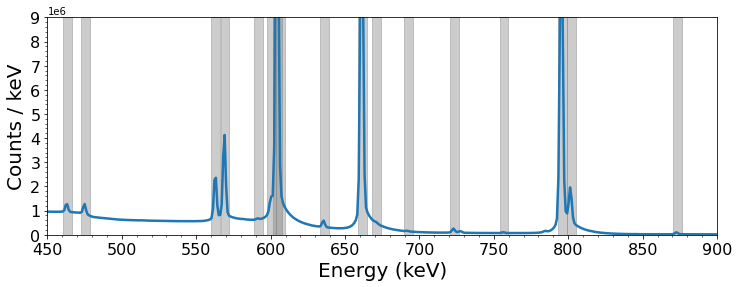
\includegraphics[width=\linewidth]{./chapters/exp2/energy_window_example.png}}
  \caption[Portion of gamma spectrum with windows, which shows summation regions 
           for spectra processing]
          {Slice of an example gamma spectrum in one of the training databases
           showing the windows over the gamma energy peaks. This is the portable
           \acrshort{HPGe} with the auto energy window list and the reference 
           sample's spectrum.}
  \label{fig:enwindows}
\end{figure}

After the three energy window lists are created, the full gamma spectra
database of a given detector are processed into three training sets, one for
each list.  Next, as previously mentioned, the energy window width for each
detector is used to sum the binned counts for each energy window list entry.
this is visualized in Figure \ref{fig:enwindows}, where a portion of a portable
\gls{HPGe} spectrum is shown with the $\pm3\:keV$ windows from the auto energy
window list.  Three training sets are created for each detector, resulting in
18 detector-based processed gamma spectra training sets.

\noindent \textbf{Step 4: Apply Statistical Counting Error}

Lastly, the fourth step involves the inclusion of the counting error for the
summed energy windows. This is quite simple mathematically speaking, as
statistical counting error of $n$ counts is $\sqrt{n}$.  As in Section
\ref{sec:inforeduc1}, this error gets applied in the same way for the
scikit-learn algorithms, where the uniform error is applied randomly within the
range $[x_i - \sqrt{x_i}, x_i + \sqrt{x_i}]$ for each summed energy window
$x_i$. For the \gls{MLL} calculations, Equation \ref{eq:mllunc} is used, where
$\sigma_{i} = \sqrt{x_i}$.  

In summary, there are four steps taken to arrive at training databases based on
gamma spectra from six chosen detectors. Unlike the simple increase in training
set error applied in Chapter \ref{ch:exp1}, each step of the process adds an
additional layer of reduced information quality, which are listed here:
\begin{enumerate}
  \item The list of nuclides is limited to manually chosen radionuclides.
  \item Instead of "perfect" radionuclide activity knowledge, they are being 
        measured by a gamma detector.
  \item The processing of the gamma spectra can be highly variable.
  \item The $\sqrt{n}$ error of counts-based detection is included. 
\end{enumerate}



\section{Statistical Learning Implementation}
\label{sec:statmodel1}

\begin{figure}[H]
  \centering
  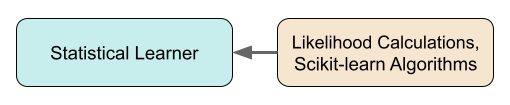
\includegraphics[width=0.7\linewidth]{./chapters/exp2/methodology2_3.png}
  \caption[Third portion of the flowchart from Figure \ref{fig:method2}]
          {Third portion of the flowchart from Figure \ref{fig:method2} being 
           described in this section.}
\end{figure}

The chosen algorithms (\textit{k}-nearest neighbors, decision trees, and
\gls{MLL} calculations) are introduced in Section \ref{sec:algs} and their
implementation details are in Section \ref{sec:statmodel1}.  This section will
therefore only cover the implementation differences from the previous work.
The \gls{MLL} calculations are implemented identically to Chapter
\ref{ch:exp1}.  However, the scikit-learn algorithms in this experiment did
undergo a new round of hyperparameter optimization.

The full list of 22 training sets that undergo training and prediction are as
follows: 
\begin{itemize}
  \item 1 set of nuclide masses (29 nuclide masses from Chapter \ref{ch:exp1})
  \item 3 sets of nuclide activities
    \begin{itemize}
      \item 32 nuclide activities (full knowledge scenario for all nuclides, 
            whether or not they are present in a quantity able to be detected)
      \item 12 nuclide activities (full knowledge for long energy windows list)
      \item 7 nuclide activities (full knowledge for short energy windows list)
    \end{itemize}
  \item 18 detector-based processed spectra sets
    \begin{itemize}
      \item Auto energy windows lists applied to six detectors (lab-based 
            \gls{HPGe}, portable \gls{HPGe}, \gls{CZT}, \gls{SrI2}, \gls{LaBr3}, 
            \gls{NaI})
      \item Short energy windows lists applied to six detectors above
      \item Long energy windows lists applied to six detectors above
    \end{itemize}
\end{itemize}

\begin{table}[!htb]
  \centering
  \begin{tabular}{@{}llcll@{}}
    \toprule
    \textbf{\begin{tabular}[c]{@{}l@{}}Training Set\\ Description\end{tabular}} &
    \textbf{\begin{tabular}[c]{@{}l@{}}Prediction\\ Parameter\end{tabular}} &
    \textbf{\begin{tabular}[c]{@{}l@{}}\textit{k} \\ (N neighbors)\end{tabular}} &
    \textbf{\begin{tabular}[c]{@{}l@{}}Max \\ Depth\end{tabular}} &
    \textbf{\begin{tabular}[c]{@{}l@{}}Max \\ Features\end{tabular}} \\ 
    \toprule
    \multirow{4}{*}{\begin{tabular}[c]
    {@{}l@{}}29 \\ Nuclide\\ Masses\end{tabular}}          & Reactor Type & 4 & 56 & 29          \\
                                                           & Burnup       & 1 & 77 & 29          \\
                                                           & Enrichment   & 1 & 73 & 29          \\
                                                           & Cooling Time & 2 & 45 & 29          \\ 
                                                           \hline
    \multirow{4}{*}{\begin{tabular}[c]
    {@{}l@{}}32\\ Nuclide\\ Activities\end{tabular}}       & Reactor Type & 1 & 41 & 32          \\
                                                           & Burnup       & 1 & 49 & 32          \\
                                                           & Enrichment   & 1 & 67 & 32          \\
                                                           & Cooling Time & 7 & 56 & 32          \\
                                                           \hline
    \multirow{4}{*}{\begin{tabular}[c]
    {@{}l@{}}7 or 12\\ Nuclide \\ Activities\end{tabular}} & Reactor Type & 1 & 67 & 7 or 12     \\
                                                           & Burnup       & 1 & 78 & 7 or 12     \\
                                                           & Enrichment   & 1 & 60 & 7 or 12     \\
                                                           & Cooling Time & 4 & 68 & 7 or 12     \\
                                                           \hline
    \multirow{4}{*}{\begin{tabular}[c]
    {@{}l@{}}Energy \\ Windows:\\ Short\end{tabular}}      & Reactor Type & 1 & 62 & 42          \\
                                                           & Burnup       & 1 & 62 & 42          \\
                                                           & Enrichment   & 4 & 64 & 42          \\
                                                           & Cooling Time & 2 & 54 & 42          \\
                                                           \hline
    \multirow{4}{*}{\begin{tabular}[c]
    {@{}l@{}}Energy \\ Windows:\\ Long\end{tabular}}       & Reactor Type & 4 & 62 & 151         \\
                                                           & Burnup       & 1 & 51 & 151         \\
                                                           & Enrichment   & 5 & 73 & 151         \\
                                                           & Cooling Time & 2 & 64 & 151         \\
                                                           \hline
    \multirow{4}{*}{\begin{tabular}[c]
    {@{}l@{}}Energy \\ Windows:\\ Auto\end{tabular}}       & Reactor Type & 2 & 61 & None or 150 \\
                                                           & Burnup       & 1 & 52 & None or 150 \\
                                                           & Enrichment   & 4 & 67 & None or 150 \\
                                                           & Cooling Time & 2 & 58 & None or 150 \\ 
    \bottomrule 
  \end{tabular}
  \caption[Optimized algorithm hyperparameters for all training sets in second 
           experiment]
          {Optimized algorithm hyperparameters; the energy lists took all 
           detectors into account.}
  \label{tbl:exp2hypparam}
\end{table}

Table \ref{tbl:exp2hypparam} lists the hyperparameter optimization results for
the 22 training sets. Because the 29 nuclide mass training set is included in
this chapter for comparison, its optimization results are also listed here.
The number of features for decision trees are not limited because the test runs
for optimization provided highly variable results. The only case where this is
not true is with the auto energy windows list for the lab-based \gls{HPGe} with
a length of 206; the maximum features for this one case are limited to 150.
Instead, optimization was carried out only on the maximum depth for decision
trees with keeping the full length of features.  This is an area that could
undergo deeper exploration than what occurs in this work, since the training
sets with large feature sets can become overfit.

The optimization took place in two rounds, where the first round had a coarser
grid of \textit{k} for \textit{k}-nearest neighbors and maximum depth for
decision trees and the second round had a finer grid of parameters. The 7 \& 12
nuclide activity training sets were optimized separately but contain averages
of the two results for the maximum depth, and the higher value of \textit{k}
when the two did not match. The \textit{k} and maximum depths were averaged
across all six detectors for each energy window list length (short, long, and
auto).  There were fairly consistent results from the short and long lists, but
the variable length of the auto-generated energy windows lists (in Table
\ref{tbl:enwindows}) gave a wider range of ideal hyperparameters.



\section{Prediction Performance Evaluation}
\label{sec:eval1}

\begin{figure}[H]
  \centering
  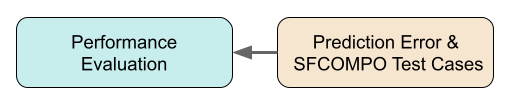
\includegraphics[width=0.7\linewidth]{./chapters/exp1/methodology1_4.png}
  \caption[Fourth portion of the flowchart from Figure \ref{fig:method1}]
          {Fourth portion of the flowchart from Figure \ref{fig:method1} being 
           described in this section.}
\end{figure}

As previously introduced in Section \ref{sec:testerr}, the prediction
performance is measured by evaluating the accuracy of the reactor type
classification or the error of the regression cases (burnup, \gls{U235}
enrichment, cooling time).  These performance metrics for all four prediction
types are compared across the three algorithms used: \textit{k}-nearest
neighbors (denoted in plots as \textit{kNN}), decision trees (denoted in plots
as \textit{Dec Tree} or \textit{DTree}), and \gls{MLL} calculations.  

\subsection{Random Error Impacts on Prediction}
\label{sec:randerr}

To judge the degradation of predictions of the algorithms with increasing
nuclide mass measurement error (i.e., reduced information quality, detailed in
Section \ref{sec:inforeduc1}), several plots are made with the introduced error
on the \textit{x}-axis and a prediction performance metric on the
\textit{y}-axis.  The \textit{y}-axis is always oriented so that lower is
poorer performance and higher is better performance. This is why Figures
\ref{fig:randburn}--\ref{fig:randcool} present a negative error on the
\textit{y}-axis. Additionally, the data points on all the plots have a small
$\Delta x$ to show error bars that are otherwise impossible to see.

In all of the results in this section, the statistics being reported is on all
$4.5 \times 10^5$ entries in the training set.

\subsubsection{Reactor Type Classification}
\label{sec:randerrA}

Figure \ref{fig:randrxtr} shows the balanced accuracy of reactor type
classification, where a score of $1$ is perfect prediction and a score of $0$
is random classification. The error bars reflect a 99\% confidence interval.
While the two scikit-learn algorithms follow a very similar path of decreased
accuracy as the error increases, the \gls{MLL} calculation approach appears to
be more robust to the nuclide mass measurement error.  Another interesting
result is that the \gls{MLL} calculation performs slightly worse for low
errors. If the expected measurement errors of nuclide masses in a training
database or in a test sample can be guaranteed to be better than ~2\%, the
\gls{MLL} calculation is no longer the obvious preferred choice for reactor
type prediction.

\begin{figure}[!htb]
  \centering
  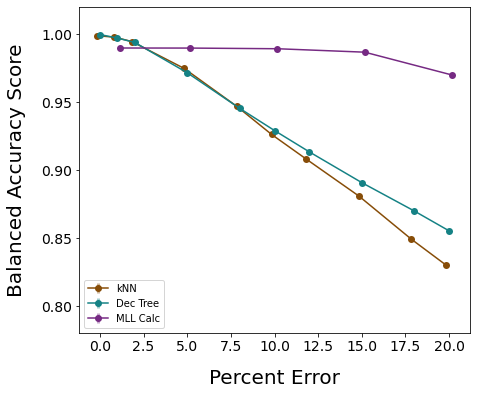
\includegraphics[width=0.5\textwidth]{./chapters/exp1/randerr_compare_nuc29_BalAcc_rxtr.png}
  \caption[Prediction performance of reactor type classification with increasing
           training set error]
          {Prediction performance of reactor type as measured by balanced 
           accuracy with respect to uniform/random error applied to the nuclide 
           mass measurements in the training set.}
  \label{fig:randrxtr}
\end{figure}

\begin{figure}[!htb]
  \centering
  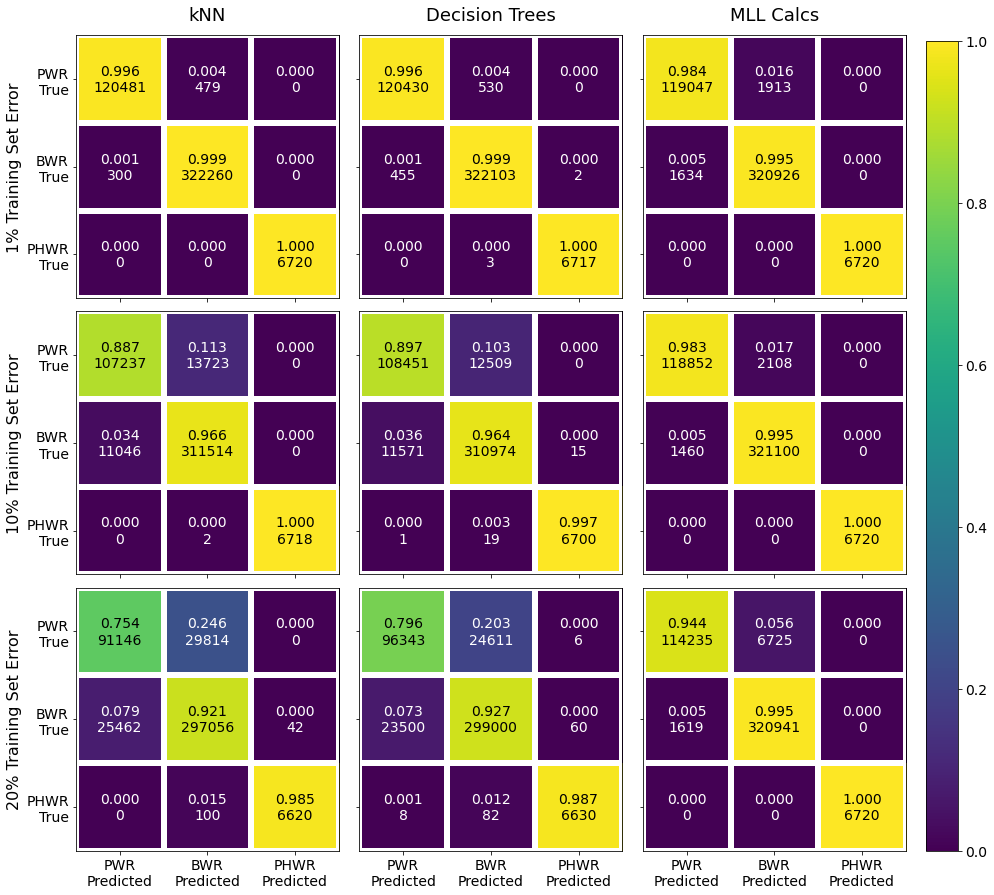
\includegraphics[width=\textwidth]{./chapters/exp1/confusion_matrix_nuc29_3errs.png}
  \caption[Confusion matrices of reactor type classification]
          {Confusion matrices of reactor type prediction for each algorithm 
           at three training set error levels: 1\%, 10\%, and 20\%, in the 
           top, middle, and bottom panels, respectively.}
  \label{fig:cm_nuc29}
\end{figure}

Although the balanced accuracy score provides more information about
classification performance for an imbalanced data set (the training set is
26.8\% \gls{PWR}, 71.6\% \gls{BWR}, and 1.5\% \gls{PHWR}), it still does not
provide much detail about what is being misclassified. To probe this further,
Figure \ref{fig:cm_nuc29} shows three sets of confusion matrices, originally
introduced in Section \ref{sec:testerr}.  The off-diagonal squares are the
fraction of false positives for each reactor type, where the predicted label
(\textit{x}-axis) is something other than the true label (\textit{y}-axis).
The false positive fractions are normalized to the number of true labels.
Below the fractions inside the pixels are the raw numbers of false positives.
The diagonal squares have three numbers in them. The top numbers are the
fraction of true positives for each reactor type (normalized to true labels),
where the predicted label (\textit{x}-axis) is equal to the true label
(\textit{y}-axis).  The middle number in parentheses is the true positive
fraction subtracted by one: $\text{TP} - 1$.  Again, the bottom number is the
raw number of true positives.  

It is ideal to have the diagonal be as close to 1 as possible and the
off-diagonal pixels be as close to 0 as possible.  To allow the fractions to be
rapidly perceived, a colorbar provides perceptually uniform shading for these
true positive and false positive fractions.  The $TP - 1$ along the diagonal is
done so that deviation from perfect classification performance of 1.0 is shaded
a different color (brown) than the off-diagonal pixels that deviate from
perfect classification performance of 0.0 (teal). Perfect performance in both
cases is the middle of the colorbar, white.  

In the top panel of Figure \ref{fig:cm_nuc29}, the three algorithms are
presented for the 1\% random error case. In Figure \ref{fig:randrxtr}, one can
see these three data points on the plot clustered near the top showing
almost-perfect performance.  (A reminder that the true positive fractions in
the confusion matrices do not map directly to the balanced accuracy score,
which puts more weight on the underrepresented classes.) The confusion matrices
give more dimension to this near-perfect reactor type classification
performance. The majority of the misclassification is in \gls{PWR}s being
classified as \gls{BWR}s: 0.4\% for \textit{k}-nearest neighbors and decision
trees, and 1.6\% for \gls{MLL} calculations. Although, there are also some
\gls{BWR}s that are misclassified as \gls{PWR}s: 0.1\% for \textit{k}-nearest
neighbors and decision trees, and 0.5\% for \gls{MLL} calculations.  There are
zero misclassified \gls{PHWR} cases and zero \gls{LWR} cases misclassified as
\gls{PHWR}; the value of 0.000 to three decimals fraction here represents a
real zero-count, but this is not necessarily the case for the other sets of
confusion matrices.  The \gls{PWR}/\gls{BWR} distinction is known to be a
difficult problem, so the correct \gls{PHWR} classifications are not
particularly notable for this discussion. 

The middle panel of Figure \ref{fig:cm_nuc29} shows confusion matrices for the
three algorithms for the 10\% random error case. In Figure \ref{fig:randrxtr},
one can see these three data points on the plot, where the \gls{MLL} point is
near a balanced accuracy score of 1, and the scikit-learn algorithms both have
score of around 0.93. As with the 1\% error case, the majority of the
misclassification is in \gls{PWR}s being classified as \gls{BWR}s: 11.3\% for
\textit{k}-nearest neighbors, 10.3\% for decision trees, and 1.7\% for
\gls{MLL} calculations.  The \gls{BWR}s are being misclassified as \gls{PWR}s
at the following percentages: 3.4\% for \textit{k}-nearest neighbors, 3.6\% for
decision trees, and 0.5\% for \gls{MLL} calculations. Note how the performance
of the \gls{MLL} calculations are nearly the same for both error levels, which
is shown by the \gls{MLL} line in Figure \ref{fig:randrxtr}. Because of the
normalization, the \gls{LWR}s that are misclassified as \gls{PHWR}s appear to
be zero. However, this does happen, just rarely: 15 \gls{BWR}s are classified
as \gls{PHWR} using decision trees. Also, \textit{k}-nearest neighbors and
decision trees misclassified \gls{PHWR} as an \gls{LWR} 2 times using the
former and 20 times using the latter (no \gls{PHWR} misclassifications happened
using \gls{MLL}).

The bottom panel of Figure \ref{fig:cm_nuc29} shows confusion matrices for the
three algorithms for the 20\% random error case. In Figure \ref{fig:randrxtr},
one can see these three data points on the plot, where the \gls{MLL} point is
near a balanced accuracy score of 0.97, \textit{k}-nearest neighbors is around
0.83, and decision trees is around 0.86. As with the previous two error cases,
the majority of the misclassification is in \gls{PWR}s being classified as
\gls{BWR}s: 24.6\% for \textit{k}-nearest neighbors, 20.3\% for decision trees,
and 5.6\% for \gls{MLL} calculations.  The \gls{BWR}s are being misclassified
as \gls{PWR}s at the following percentages: 7.9\% for \textit{k}-nearest
neighbors, 7.3\% for decision trees, and 0.5\% for \gls{MLL} calculations.
\Gls{PHWR}s are misclassified as an \gls{LWR} 100 times for \textit{k}-nearest
neighbors, 82 times for decision trees, and 0 times for \gls{MLL} calculations.
\Gls{LWR}s were misclassified as \gls{PHWR} 42 times for \textit{k}-nearest
neighbors, 66 times for decision trees, and 0 times for \gls{MLL} calculations.

\subsubsection{Regression Results}
\label{sec:randerrB}

Each set of plots for a given prediction parameter in this section shows both
the relative error (\gls{MAPE}) and the absolute error (\gls{MAE}). In addition
to the \gls{MAE} on the second plot for each regression case, the \gls{MedAE}
is represented as a triangle on the plot as well. These three errors taken
together provide more detailed information about the performance of each
algorithm when faced with training set noise.  As previously mentioned, the
\textit{x}-axis has negative errors, so that higher is always better.  

\begin{figure}[!htb]
  \centering
  \begin{subfigure}[b]{0.48\textwidth}
    \centering
    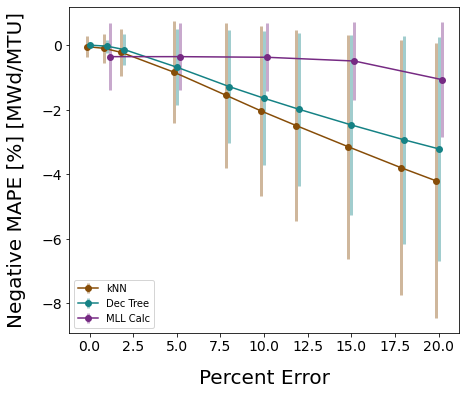
\includegraphics[width=\textwidth]{./chapters/exp1/randerr_compare_nuc29_MAPE_burn.png}
    \caption{Negative \gls{MAPE} of burnup regression with respect to 
             random error.}
    \label{fig:burnmape}
  \end{subfigure}
  \hfill
  \begin{subfigure}[b]{0.5\textwidth}
    \centering
    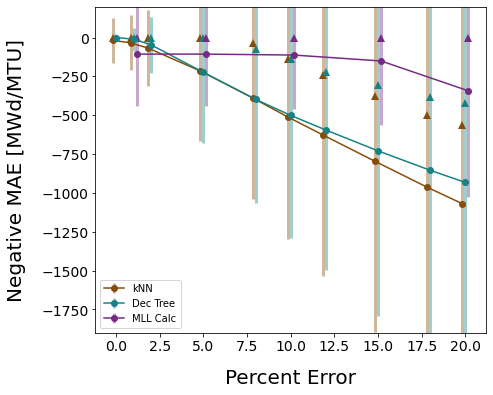
\includegraphics[width=\textwidth]{./chapters/exp1/randerr_compare_nuc29_MAE_burn.png}
    \caption{Negative \gls{MAE} of burnup regression with respect to 
             random error.}
    \label{fig:burnmae}
  \end{subfigure}
  \caption[Prediction performance of burnup regression with increasing training 
           set error]
          {Prediction performance of burnup as measured by relative and 
           absolute errors with respect to uniform/random error applied to the 
           nuclide mass measurements in the training set.}
  \label{fig:randburn}
\end{figure}

Figure \ref{fig:randburn} demonstrates the burnup prediction performance, with
the \gls{MAPE} in Figure \ref{fig:burnmape} and the \gls{MAE} and \gls{MedAE}
in Figure \ref{fig:burnmae}. In these figures, the error bars reflect one
standard deviation of the percentage errors or the absolute errors,
respectively.  As with the reactor type prediction in Figure
\ref{fig:randrxtr}, the \gls{MLL} method is robust to training set error but
performs slightly worse at low error values.  All three methods calculate
burnup with a maximum error of -5\% or $-1000\:MWd/MTU$ at 20\% error in the
training set. The \gls{MedAE}s show a more encouraging picture of the
performance as compared to the \gls{MAE}s. It is interesting that the
scikit-learn algorithms and the \gls{MLL} calculations diverge at 5\% training
set error for \gls{MAPE} and \gls{MAE}, but at 10\% training set error for the
\gls{MedAE}.

\begin{figure}[!htb]
  \centering
  \begin{subfigure}[b]{0.49\textwidth}
    \centering
    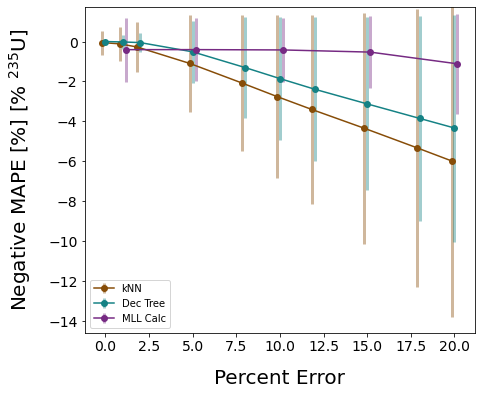
\includegraphics[width=\textwidth]{./chapters/exp1/randerr_compare_nuc29_MAPE_enri.png}
    \caption{Negative \gls{MAPE} of \gls{U235} enrichment regression with 
             respect to random error.}
    \label{fig:enrimape}
  \end{subfigure}
  \hfill
  \begin{subfigure}[b]{0.49\textwidth}
    \centering
    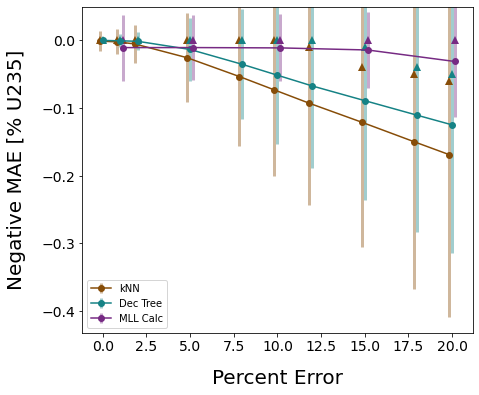
\includegraphics[width=\textwidth]{./chapters/exp1/randerr_compare_nuc29_MAE_enri.png}
    \caption{Negative \gls{MAE} of \gls{U235} enrichment regression with 
             respect to random error.}
    \label{fig:enrimae}
  \end{subfigure}
  \caption[Prediction performance of enrichment regression with increasing 
           training set error]
          {Prediction performance of enrichment as measured by relative and 
           absolute errors with respect to uniform/random error applied to the 
           nuclide mass measurements in the training set.}
  \label{fig:randenri}
\end{figure}  

Figure \ref{fig:randenri} demonstrates the \gls{U235} enrichment prediction
performance, with the \gls{MAPE} in Figure \ref{fig:enrimape} and the \gls{MAE}
and \gls{MedAE} in Figure \ref{fig:enrimae}. In these figures, the error bars
reflect one standard deviation of the percentage errors or the absolute errors,
respectively.  Again, the \gls{MLL} method is robust to training set error but
performs slightly worse at low error values.  All three methods calculate
enrichment with a maximum error of -6\% or $-0.17\:\%U235$ at 20\% error in the
training set. Again, the \gls{MedAE}s show a more encouraging picture of the
performance as compared to the \gls{MAE}s. The scikit-learn algorithms and the
\gls{MLL} calculations diverge at 10\% training set error for \gls{MAPE} and
\gls{MAE}, but at 15\% training set error for the \gls{MedAE}.

\begin{figure}[!htb]
  \centering
  \begin{subfigure}[b]{0.49\textwidth}
    \centering
    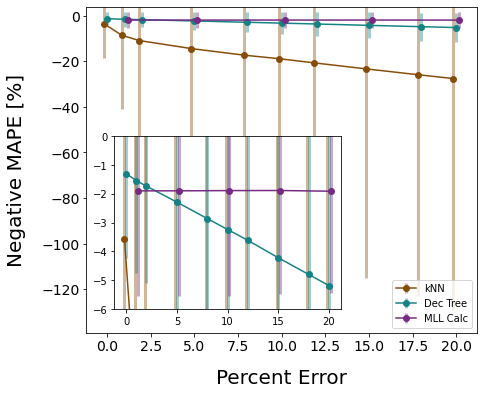
\includegraphics[width=\textwidth]{./chapters/exp1/randerr_compare_nuc29_MAPE_cool.png}
    \caption{Negative \gls{MAPE} of time since irradiation regression with 
             respect to random error.} 
    \label{fig:coolmape}
  \end{subfigure}
  \hfill
  \begin{subfigure}[b]{0.49\textwidth}
    \centering
    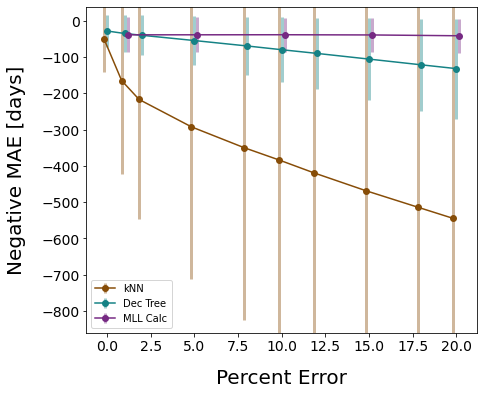
\includegraphics[width=\textwidth]{./chapters/exp1/randerr_compare_nuc29_MAE_cool.png}
    \caption{Negative \gls{MAE} of time since irradiation regression with 
             respect to random error.} 
    \label{fig:coolmae}
  \end{subfigure}
  \caption[Prediction performance of time since irradiation regression with 
           increasing training set error]
          {Prediction performance of time since irradiation as measured by 
           relative and absolute errors with respect to uniform/random error 
           applied to the nuclide mass measurements in the training set.}
  \label{fig:randcool}
\end{figure}

Last, the time since irradiation prediction performance for the three
algorithms with respect to increasing nuclide mass error is pictured in Figure
\ref{fig:randcool}.  The \gls{MAPE} is shown in Figure \ref{fig:enrimape} and
the \gls{MAE} and \gls{MedAE} are shown in Figure \ref{fig:enrimae}.  The error
bars reflect one standard deviation of the percentage errors or the absolute
errors, respectively.  The \gls{MLL} method is most robust to training set
error, but for this prediction parameter, the behavior of \textit{k}-nearest
neighbors is unique here versus the previous two regression categories.  Time
since irradiation is predicted with a maximum error of -30\% or $-550\:days$ at
20\% error in the training set using the \textit{k}-nearest neighbors
algorithm.  In Figure \ref{fig:coolmape}, there is an inset to show more detail
about the behavior of the decision trees and \gls{MLL} calculations curves, so
if one ignores the clearly anomalous \textit{k}-nearest neighbors performance
and focuses instead on decision trees, those values are -6\% and $-120\:days$.
The \gls{MLL} calculations remain nearly horizontal at approximately 2\%
prediction error for all training set error levels.  The \gls{MedAE}, as usual,
shows a more encouraging picture of the performance as compared to the
\gls{MAE}.

Overall, the robustness to training set error that is present in the \gls{MLL}
calculations applies to all of the prediction parameters. The decision trees
performance is second best, and \textit{k}-nearest neighbors performs the
worst.  In the case of time since irradiation, \textit{k}-nearest neighbors
degrades incredibly fast with introduced training set error.  While it is
difficult to draw a baseline for minimum acceptable behavior on these plots,
these performances can serve as a benchmark for the work presented in Chapter
\ref{ch:exp2}. 


\subsubsection{Model Generalization}
\label{sec:randerrC}

Although a key takeaway from Section \ref{sec:randerr} is that the \gls{MLL}
calculations are the most resilient to introduced error in the training set
features for all four prediction categories, there is another aspect of the
algorithm performance not explicitly shown in those plots: generalization.
\Gls{MLL} does not generalize to unseen data; it provides predictions based on
finding the closest training set entry to the test sample.  It (usually)
outperforms the scikit-learn methods in part because the training set is so
large. This is also true for the \textit{k}-nearest neighbor implementations
where $k=1$ (burnup and cooling time, as seen in Table \ref{tbl:exp1hypparam}).

\begin{figure}[!htb]
  \centering
  \begin{subfigure}[b]{0.495\textwidth}
    \centering
    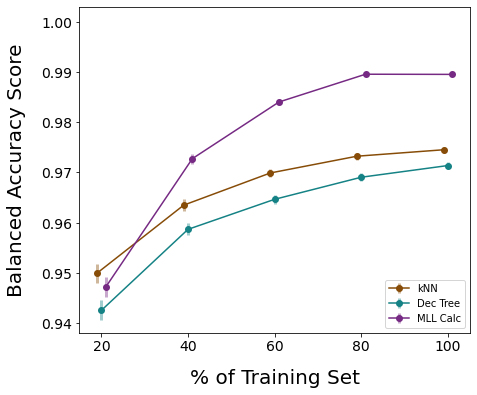
\includegraphics[width=\textwidth]{./chapters/exp1/learncurve_nuc29_err05_BalAcc_rxtr.png}
    \caption{Balanced accuracy of reactor type classification with respect 
             to training set size.}
    \label{fig:learnsA}
  \end{subfigure}
  \hfill
  \begin{subfigure}[b]{0.485\textwidth}
    \centering
    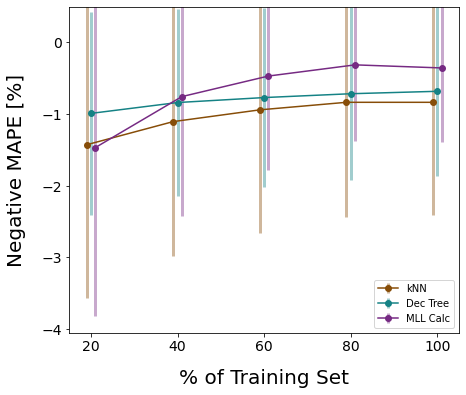
\includegraphics[width=\textwidth]{./chapters/exp1/learncurve_nuc29_err05_MAPE_burn.png}
    \caption{Negative \gls{MAPE} of burnup regression with respect to 
             to training set size.}
    \label{fig:learnsB}
  \end{subfigure}
  \vskip\baselineskip
  \begin{subfigure}[b]{0.48\textwidth}
    \centering
    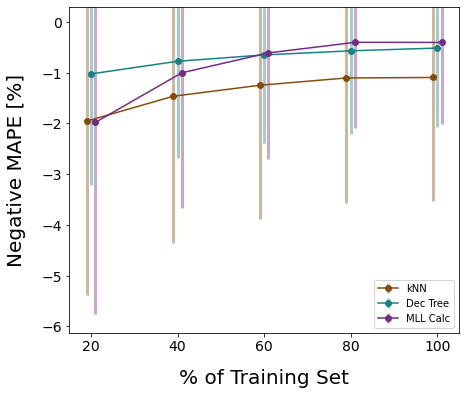
\includegraphics[width=\textwidth]{./chapters/exp1/learncurve_nuc29_err05_MAPE_enri.png}
    \caption{Negative \gls{MAPE} of \gls{U235} enrichment regression with 
             respect to training set size.}
    \label{fig:learnsC}
  \end{subfigure}
  \hfill
  \begin{subfigure}[b]{0.50\textwidth}
    \centering
    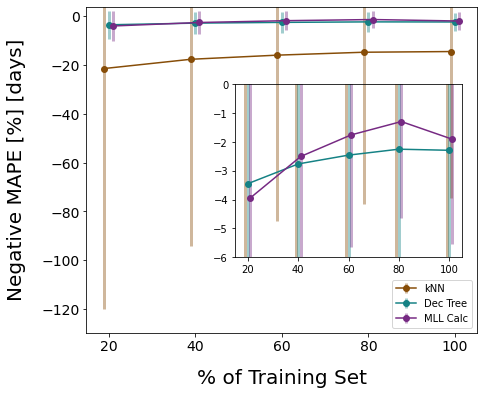
\includegraphics[width=\textwidth]{./chapters/exp1/learncurve_nuc29_err05_MAPE_cool.png}
    \caption{Negative \gls{MAPE} of time since irradiation regression with 
             respect to training set size.}
    \label{fig:learnsD}
  \end{subfigure}
  \caption[Learning curves for all four prediction parameters]
          {Learning curves for reactor type, burnup, enrichment, and time 
           since irradiation with respect to increasing fraction of the 
           training set, for 5\% training set random error.}
  \label{fig:learns}
\end{figure}

One way to show that an algorithm is generalizing well in comparison to others
is to view the shape of its learning curve (introduced in Section
\ref{sec:complexity}): the prediction performance with respect to training set
size.  It is crucial to have the training sets be identical for each algorithm,
so they were created in advance and the learning curves are constructed
manually rather than relying on the scikit-learn method.  Smaller training sets
were created from the original one by taking 80\%, 60\%, 40\%, and 20\% of the
entries. The training sets are all stratified so that the original fractions of
\gls{BWR}, \gls{PWR}, and \gls{PHWR} are retained. They are also built on top
of one another, so the 20\%-size training set is contained within the 40\%-size
set, and so forth.

Learning curves were constructed for all four prediction categories,
demonstrated in Figure \ref{fig:learns}. As in Figures
\ref{fig:randrxtr}--\ref{fig:randcool} , the vertical axis is always oriented
so that lower is poorer performance and higher is better performance; also, the
error bars reflect a 99\% confidence interval for Figure \ref{fig:learnsA}, and
one standard deviation of the average percentage errors for Figures
\ref{fig:learnsB}--\ref{fig:learnsD}.  These learning curves represent the 5\%
random error case in Figures \ref{fig:randrxtr}--\ref{fig:randcool}, so the
scores/errors in these figures are the data points at the 100\% training set
level in Figure \ref{fig:learns}.  Therefore, the leftmost data in Figure
\ref{fig:learns} will show the \gls{MLL} point being slightly above the
scikit-learn points for the reactor type, burnup, and enrichment predictions,
and the \textit{k}-nearest neighbor point is below the \gls{MLL} and decision
trees points for time since irradiation.  

Figure \ref{fig:learnsA} shows that the balanced accuracy score of reactor type
classification for the \gls{MLL} calculations decreases more at lower training
set size than for the scikit-learn algorithms. Here, the curve crosses below
the \textit{k}-nearest neighbors curve at the lowest training set size of 20\%.
For the burnup \gls{MAPE} in Figure \ref{fig:learnsB} and the enrichment
\gls{MAPE} in Figure \ref{fig:learnsC}, the \gls{MLL} curve crosses below both
of the scikit-learn algorithm curves. This happens between 20\% and 40\%
training set size for burnup, and between 40\% and 60\% training set size for
enrichment.  Lastly, Figure \ref{fig:learnsD} shows a different arrangement,
which is to be expected from the results shown in Figure \ref{fig:randcool},
where the \textit{k}-nearest neighbors performance is significantly worse than
the other two algorithms. Because the \textit{k}-nearest neighbors curve and
error bars are so large, there is an inset showing a closeup of the other two
curves above -6\%.  The decision trees and \gls{MLL} calculations curves now
appear to follow the trend in the burnup and enrichment cases, and the
\gls{MLL} curve crosses under the decision trees curve between 20\% and 40\%
training set size.  

There is a dependence on training set size for all three algorithms in Figure
\ref{fig:learns}. For the most part, the \textit{k}-nearest neighbors and
decision trees curves follow an approximately parallel path, whereas the
\gls{MLL} method shows an increased rate of degradation at low training set
sizes. Since this training set is large enough, i.e., the prediction parameters
were included in small enough steps, that \gls{MLL} has consistent performance
at the larger sizes, there is not a concern in this work about its inability to
generalize. It must be noted, however, that the \gls{MLL} approach requires a
fine grid of simulation parameters in a training database to perform better
than the simple scikit-learn algorithms.

\subsubsection{Reactor Type Prior Knowledge}
\label{sec:randerrD}

There is similar work being done to this work that focuses on similar
prediction categories but in a serial manner, i.e., first determining the
reactor type before moving forward with other predictions \cite{serial_ml}.
This work predicts reactor operation parameters while blind to the reactor
type, but it makes sense intuitively that having previous knowledge of the
reactor type would allow more accurate regression of these parameters.
Therefore, the change in regression performance from the reactor type-blind
predictions to having prior knowledge of the reactor type is discussed.

The workflow was repeated for the three regression cases where they were
trained on reactor type-specific training sets. A 5\% random error was applied
to these training sets, and the 5\% random error full training set was used as
comparison. The errors for each algorithm (\textit{k}-nearest neighbors,
decision trees, and \gls{MLL} calculations) were tallied for each regression
category (burnup, enrichment, and time since irradiation) and within that, for
each reactor type (\gls{PWR}, \gls{BWR}, \gls{PHWR}). Two sets of error were
tracked: whether the reactor type was \textit{known} or \textit{unknown} prior
to prediction.

Table \ref{tbl:knownrxtr} shows the \gls{MAPE}s for each regression category
and within that, for each reactor type (\gls{PWR}, \gls{BWR}, \gls{PHWR}).  The
columns are separated first by the algorithms and second by whether the reactor
type was known or unknown prior to prediction, denoted as \textit{K} and
\textit{U}, respectively. Most of these relative errors are quite low, and
around or under 2\%.  So, e.g., despite burnup prediction from \glspl{PHWR}s
improving, it was by 0.61\%, a precision of which may not be of concern. Still,
these performance differences can be looked at in more detail.  

\begin{table}[!htb]
  \centering
  \begin{tabular}{@{}llllllll@{}}
    \toprule
    &  &  \multicolumn{2}{c}{\textit{k}NN} 
    &     \multicolumn{2}{c}{Dec Trees} 
    &     \multicolumn{2}{c}{MLL Calcs} \\ 
    \toprule
    \begin{tabular}[c]{@{}l@{}}Prediction\\ Parameter\end{tabular} &
    \begin{tabular}[c]{@{}l@{}}Reactor \\ Type\end{tabular} &
    K & U &  K & U & K & U \\ \midrule
    \multirow{3}{*}{\begin{tabular}[c]{@{}l@{}}Burnup \\ \% {$[MWd/MTU]$} \end{tabular}}
     & PWR  & 0.60  & 0.66  & 0.54 & 0.75 & 0.24 & 0.25 \\
     & BWR  & 0.88  & 0.90  & 0.60 & 0.66 & 0.40 & 0.40 \\
     & PHWR & 0.66  & 1.27  & 0.14 & 0.54 & 0.28 & 0.28 \\ \hline
    \multirow{3}{*}{\begin{tabular}[c]{@{}l@{}}Enrichment \\ \% {$[\%\:{}^{235}\text{U}]$} \end{tabular}}
     & PWR  & 0.85  & 0.99  & 0.36 & 0.48 & 0.26 & 0.29 \\
     & BWR  & 1.14  & 1.16  & 0.51 & 0.54 & 0.45 & 0.46 \\
     & PHWR & 0.00  & 0.00  & 0.00 & 0.02 & 0.00 & 0.00 \\ \hline
    \multirow{3}{*}{\begin{tabular}[c]{@{}l@{}}Time Since \\ Irradiation \\ \% {$[days]$} \end{tabular}}
     & PWR  & 11.44 & 10.48 & 2.35 & 2.19 & 1.55 & 1.46 \\
     & BWR  & 15.39 & 15.48 & 2.27 & 2.28 & 2.06 & 2.05 \\
     & PHWR & 19.32 & 34.41 & 4.96 & 4.52 & 2.30 & 2.30 \\ \bottomrule
  \end{tabular}
  \caption[\acrshort{MAPE}s for three regression cases comparing known versus 
           unknown reactor type prior knowledge]
          {\acrshort{MAPE}s for the three prediction cases for each algorithm 
           at 5\% training set error. \textit{K} refers to \textit{known} 
           reactor type and \textit{U} refers to \textit{unknown} reactor type 
           prior to regression.}
  \label{tbl:knownrxtr}
\end{table}

To better see these performance differences, the percent change in prediction
\gls{MAE} for each algorithm and reactor type between the reactor type being
known versus unknown prior to prediction was calculated as: $100 \cdot
\frac{MAE_{unknown} - MAE_{known}}{MAE_{unknown}}$.  This was chosen to be
relative to the unknown error since that is the benchmark in this case.  Figure
\ref{fig:knownrxtr} is three heatmaps that show this percent change for each
prediction category, algorithm, and reactor type.  This value is reflected by a
diverging color bar as well as a positive or negative percentage in each
square.  The positive percentages indicate the error decreased/improved from
the unknown reactor type case to the known reactor type case.  The negative
percentages indicate the error increased/worsened from the unknown to the known
case. 

\begin{figure}[!htb]
  \centering
  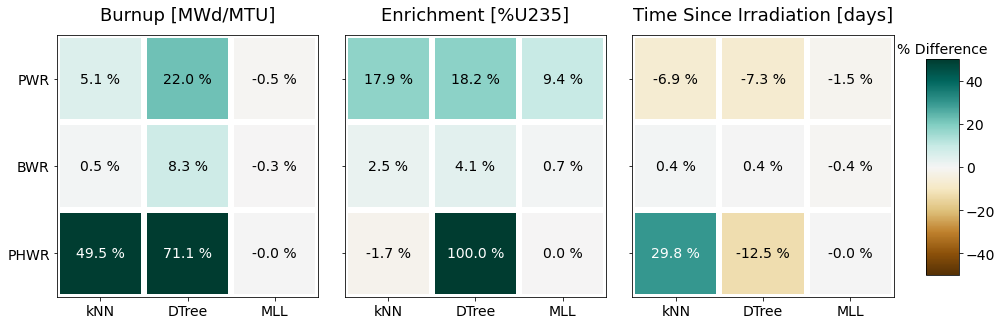
\includegraphics[width=\textwidth]{./chapters/exp1/rxtr-type_known-unknown_diff_err05.png}
  \caption[Heatmaps for three regression cases comparing known versus 
           unknown reactor type prior knowledge]
          {Heatmaps for the three regression cases showing the percent 
           difference in prediction error between a known reactor type 
           and unknown reactor type using a 5\% training set error.}
  \todo[inline]{would this be better shown with a plot that has little arrows? or leave like this?}
  \label{fig:knownrxtr}
\end{figure}

For burnup prediction, most differences are within $\pm10\%$ except for three
scenarios.  The decision tree algorithm has improved burnup prediction for
\glspl{PWR}s by 22.0\% and for \glspl{PHWR}s by 71.1\% given a known reactor
type.  The \textit{k}-nearest neighbors algorithm has 49.5\% improved burnup
prediction for the \gls{PHWR}. For \gls{U235} enrichment, the \gls{PWR}
predictions improve by approximately 18\% for the scikit-learn algorithms.
Even though the value is within $\pm10\%$, this is the only scenario where
there is an appreciable difference in \gls{MLL} performance. The decision tree
enrichment prediction of \glspl{PHWR}s also has a sizeable improvement of
100.0\%.  The time since irradiation predictions for the most part do not show
improvement outside of $\pm10\%$. Of note is some volatile behavior for the
\gls{PHWR} case with the scikit-learn algorithms.  While \textit{k}-nearest
neighbors improves by 29.8\%, the decision tree predictions were worse by
12.5\%.  Since the main concern here is showing how prediction performance
improves with prior reactor type knowledge, this reduction in performance is
odd but not worthy of further investigation.

The improvements in the \gls{PHWR} predictions are not surprising since the
generalization of the scikit-learn algorithms could lead to the unique
\gls{PHWR} cases being ignored, since they are after all only 1.5\% of the
training set.  Another interesting result is that the \gls{BWR} predictions
experience no large changes, which makes sense given that they comprise 72\% of
the training set. Also, the \gls{MLL} predictions are approximately the same,
which is expected because this algorithm does not generalize, and the
prediction comes as a set of labels and is therefore already linked to the
reactor type. Overall, it is important to be aware that the regression labels
coming from a \gls{PHWR} will be unlikely to be optimal results (except for
those from \gls{MLL} calculations).

%\begin{table}[!htb]
%  \centering
%  \begin{tabular}{@{}llllllll@{}}
%    \toprule
%    &  &  \multicolumn{2}{c}{\textit{k}NN} 
%    &     \multicolumn{2}{c}{Dec Trees} 
%    &     \multicolumn{2}{c}{MLL Calcs} \\ 
%    \toprule
%    \begin{tabular}[c]{@{}l@{}}Prediction\\ Parameter\end{tabular} &
%    \begin{tabular}[c]{@{}l@{}}Reactor \\ Type\end{tabular} &
%    K & U &  K & U & K & U \\ \midrule
%    \multirow{3}{*}{\begin{tabular}[c]{@{}l@{}}Burnup \\ \% {$[MWd/MTU]$} \end{tabular}}
%     & PWR  & 0.08  & 0.08  & 0.03 & 0.04 & 0.24 & 0.25 \\ 
%     & BWR  & 0.11  & 0.10  & 0.03 & 0.03 & 0.40 & 0.40 \\ 
%     & PHWR & 0.13  & 0.19  & 0.01 & 0.03 & 0.29 & 0.29 \\ \hline
%    \multirow{3}{*}{\begin{tabular}[c]{@{}l@{}}Enrichment \\ \% {$[\%\:{}^{235}\text{U}]$} \end{tabular}}
%     & PWR  & 0.10  & 0.11  & 0.02 & 0.02 & 0.26 & 0.29 \\ 
%     & BWR  & 0.12  & 0.12  & 0.02 & 0.02 & 0.46 & 0.46 \\ 
%     & PHWR & 0.00  & 0.00  & 0.00 & 0.00 & 0.00 & 0.00 \\ \hline
%    \multirow{3}{*}{\begin{tabular}[c]{@{}l@{}}Time Since \\ Irradiation \\ \% {$[days]$} \end{tabular}}
%     & PWR  & 6.47  & 6.13  & 1.50 & 1.43 & 1.55 & 1.46 \\ 
%     & BWR  & 9.18  & 9.15  & 1.56 & 1.53 & 2.07 & 2.05 \\ 
%     & PHWR & 13.78 & 18.62 & 4.51 & 3.71 & 2.30 & 2.30 \\ \bottomrule
%  \end{tabular}
%  \caption{\gls{MAPE}s for the three prediction cases for each algorithm at 1\% 
%           training set error. \textit{K} refers to \textit{known} reactor 
%           type and \textit{U} refers to \textit{unknown} reactor type prior 
%           to regression.}
%  \label{tbl:knownrxtr}
%\end{table}

%\begin{figure}[!htb]
%  \centering
%  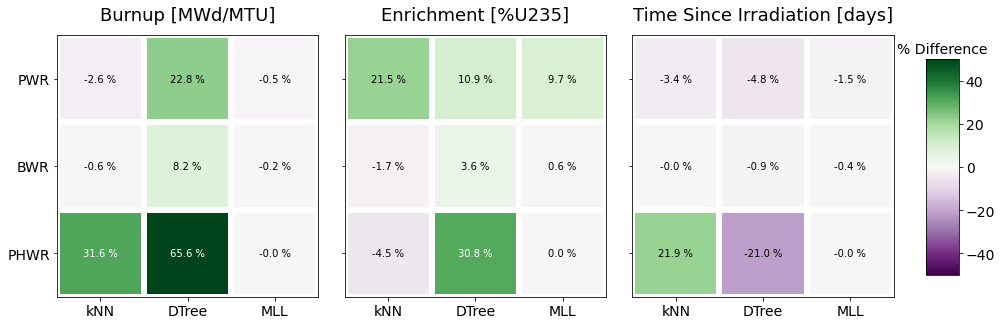
\includegraphics[width=\textwidth]{./chapters/exp1/rxtr-type_known-unknown_diff_err01.png}
%  \caption{Heatmaps for the three regression cases showing the percent 
%           difference in prediction error between a known reactor type 
%           and unknown reactor type.}
%  \label{fig:knownrxtr}
%\end{figure}



\subsection{SFCOMPO Test Set}
\label{sec:sfcompo}

\todo[inline]{1. all of my commentary on performance improvement for the
sfcompo test set is outlined to go into the future work section. or should it
go here?  2. also, there may be some useful information from the model
generalization or rxtr type prior knowledge sections that could be useful here
for more in depth discussion. 3. this ended up really motivating the use of
relative error versus absolute (really, both) so it could maybe go first, then
the random error results section could go second using the relative error
plots?}

The testing described in Section \ref{sec:randerr} describes the process of
evaluating the methodology with test cases drawn from the training database.
It is also helpful to test the methodology against real assays of \gls{SNF}.
The \gls{SFCOMPO} database was created to allow access to these sorts of
measurements linked to the reactor operation parameters being predicted in this
work. \cite{sfcompo}. The only parameter not part of the \gls{SFCOMPO} database
is the time since irradiation, so that is not predicted here. 

\begin{figure}[!htb]
  \centering
  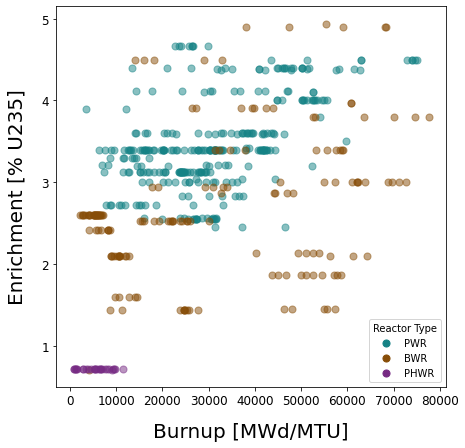
\includegraphics[width=0.7\textwidth]{./chapters/exp1/sfcompo_scatter_viz.png}
  \caption{Scatter plot showing the range of reactor operation parameters in 
           the \gls{SFCOMPO} testing set that are being predicted.}
  \label{fig:sfcoscatter}
  \todo[inline]{maybe show comparison against training E v B scatter plot}
\end{figure}

There are 505 test cases that are able to be compared against the training
database.  The number of each reactor type is as follows: 312 \gls{PWR}s, 165
\gls{BWR}s, and 28 \gls{PHWR}s. The space of enrichment and burnup values is
visualized in Figure \ref{fig:sfcoscatter}. These are sufficiently represented
in the training set design, as pictured in Figure \ref{fig:trainhist}, although
the proportions of \gls{PWR} and \gls{BWR} are approximately opposite to the
training set. The assays in \gls{SFCOMPO} are presented as nuclide
concentrations with the units \textit{milligrams per grams of initial uranium},
or $mg/gU_i$. The training set of nuclide measurements in \textit{grams} is
converted to these concentration units prior to prediction is converted to
these concentration units prior to prediction. 

There is one main issue with using \gls{SFCOMPO} as a testing set: missing
nuclide measurements.  The feature set of 29 nuclides in Table
\ref{tbl:nucmass} was chosen based on the frequency of these measurements being
present in the database at an arbitrary level of 100 measurements. This
happened before filtering, so there are some nuclide measurements present at
under 100 counts.  Each nuclide's frequency in \gls{SFCOMPO} is listed in Table
\ref{tbl:missing}.  While every assay contains several plutonium measurements
and most contain uranium measurements as well, the remaining nuclides are
present at a much lower rate. 

\begin{table}[!htb]
  \centering
  \begin{tabular}{>{\raggedleft}m{0.6in}
                                m{0.4in}
                  >{\raggedleft}m{0.6in}
                                m{0.4in}
                  >{\raggedleft}m{0.6in}
                                m{0.4in}}
    \toprule
    \rowcolor[gray]{0.88} am241  & 237 & nd145 & 162 & sm147 & 97  \\  
    \rowcolor[gray]{0.95} am242m & 110 & nd146 & 139 & sm149 & 97  \\ 
    \rowcolor[gray]{0.88} am243  & 203 & nd148 & 275 & sm150 & 97  \\ 
    \rowcolor[gray]{0.95} cm242  & 214 & nd150 & 121 & sm151 & 97  \\ 
    \rowcolor[gray]{0.88} cm244  & 269 & np237 & 155 & sm152 & 97  \\ 
    \rowcolor[gray]{0.95} cs134  & 113 & pu238 & 369 & u234  & 355 \\ 
    \rowcolor[gray]{0.88} cs137  & 185 & pu239 & 505 & u235  & 479 \\ 
    \rowcolor[gray]{0.95} eu154  & 100 & pu240 & 505 & u236  & 462 \\ 
    \rowcolor[gray]{0.88} nd143  & 162 & pu241 & 504 & u238  & 433 \\ 
    \rowcolor[gray]{0.95} nd144  & 113 & pu242 & 505 &       &     \\ \bottomrule
  \end{tabular}
  \caption{Number of assays each nuclide is measured for in the \gls{SFCOMPO}
           database.}
  \label{tbl:missing}
\end{table}

Although some algorithms in theory can handle null values in the training
stage, scikit-learn does not currently include this capability. The \gls{MLL}
method is designed to handle null values, however. This is done by converting
them to zero and filtering out all zero-valued nuclides during the likelihood
calculations. But there is a technique more commonly applied than converting
missing values to zero: imputation. This involves taking the mean or median of
the existing features and applying that value to the assays in which it is
missing.  The remainder of this section dicusses using the three algorithms to
predict the \gls{SFCOMPO} test cases where the nulls are both converted to zero
and imputed using the mean.  \todo[inline]{is converting to zero technically
imputation as well?}

\subsubsection{Reactor Type Classification}

Table \ref{tbl:sfcorxtr} presents two metrics for the two missing value
techniques: the accuracy and balanced accuracy scores. The accuracy scores for
both the imputed nulls and zero-nulls test sets are mostly under 0.62, which is
the fraction of \gls{PWR} entries.  Therefore, a classifier could predict
\gls{PWR} every time and do better than these accuracy scores.  For the
zero-nulls test set predictions using \gls{MLL}, however, the accuracy of 0.72
does exceed the "majority guess" accuracy of 0.62.  Since \gls{MLL}
calculations filter out null values, it is expected that the scores will be
higher for all prediction categories where \gls{MLL} is being used with the
zero-nulls test set. This expected \gls{MLL} performance also holds true when
looking at the balanced accuracy score.  A balanced accuracy score of 0 denotes
random guessing, but it can also be negative if the classifications are worse
than random guessing. The balanced accuracy of 0.63 for the zero-nulls case is
a promising result. The balanced accuracies of \textit{k}-nearest neighbors and
decision trees are all quite low. Also, the higher accuracies correspond to lower
balanced accuracies, and vice versa. Therefore, further investigation is
necessary.

\begin{table}[!htb]
  \centering
  \begin{tabular}{@{}m{1.5in}llllll@{}}
    \toprule
    & \multicolumn{3}{m{2in}}{Accuracy Scores} 
    & \multicolumn{3}{l}{Balanced Accuracy Scores} \\ 
    \toprule
    Null Handling    & kNN   & DTree  & MLL   & kNN   & DTree  & MLL    \\ \midrule
    Imputed Nulls    & 0.52  & 0.60   & 0.39  & 0.09  & 0.12   & -0.01  \\
    Zero-value Nulls & 0.45  & 0.42   & 0.72  & 0.21  & 0.30   & 0.63   \\ \bottomrule
    \end{tabular}
  \caption{Accuracy and balanced accuracy scores for reactor type prediction 
           of the \gls{SFCOMPO} test cases.}
  \label{tbl:sfcorxtr}
\end{table}

\begin{figure}[!htb]
  \centering
  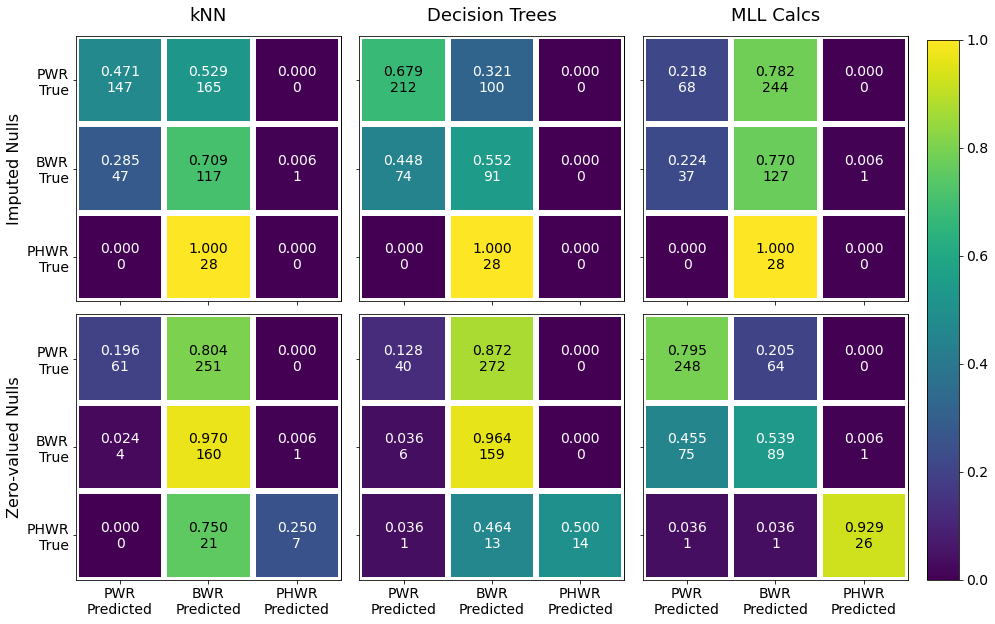
\includegraphics[width=\textwidth]{./chapters/exp1/confusion_matrix_sfco.png}
  \caption{Confusion matrices of reactor type prediction for each algorithm 
           using two missing entry techniques: imputation with mean values (top 
           panel) and replacement with zero (bottom panel).}
  \label{fig:cm}
\end{figure}

Figure \ref{fig:cm} allows for a deeper look into what is happening with the
reactor type predictions for both of the \gls{SFCOMPO} test sets.  The matrices
from using mean-imputed null values are in the top panel and the matrices from
using zero-filled null values are in the bottom panel.  The scikit-learn
algorithms have a higher accuracy for the imputed null values test set than
their zero-null values counterparts, but the balanced accuracies follow the
opposite direction. For \textit{k}-nearest neighbors, imputed nulls cause more
than half of the \gls{PWR}s and all of the \gls{PHWR}s to be misclassified as
\gls{BWR}s. Additionally, 28.5\% \gls{BWR}s are misclassified as \gls{PWR}s.
For the zero-nulls test set, there is a much larger correct \gls{BWR}
classification percentage, but also a much larger \gls{PWR} misclassification
percentage. The \gls{PHWR} true positive percentage increases from 0 to 25\%.
\Gls{BWR} (32\% of test cases) and \gls{PHWR} (5.5\% of test cases) are the two
minority classes in the database.  Because they both have higher true positive
fractions but there were overall fewer correct predictions (from a much higher
\gls{PWR} misclassification) from the imputed nulls to the zero-nulls, the
accuracy went down but the balanced accuracy went up.

Decision trees follows a similar pattern the the \textit{k}-nearest neighbors
example.  The \gls{PWR} misclassification increases from the imputed nulls to
the zero-nulls test set in a similar manner, although the original \gls{PWR}
true positive fraction is higher (leading to a higher accuracy for the imputed
nulls case).  As before, the \gls{BWR} correct classification increases
drastically from the imputed nulls to zero-nulls case.  Additionally, the
\gls{PHWR} classifiction improvement from imputed nulls to zero-nulls is better
for decision trees than for \textit{k}-nearest neighbors.  Therefore, again,
the accuracy decreased and the balanced accuracy increased. The larger
improvement for the minority classes has led to the larger balanced accuracy
improvement for decision trees.

In Figure \ref{fig:cm}, the confusion matrices for the \gls{MLL} calculations
tell a very different story than those for the scikit-learn algorithms.  The
only similarity is that using imputed nulls causes all \gls{PHWR}s to be
classified as \gls{BWR}s. \gls{PWR}s are misclassified as \gls{BWR}s at 78.2\%,
and \gls{BWR}s are misclassified as \gls{PWR}s at 22.4\%. For the zero-nulls
test set, \gls{PHWR}s and \gls{PWR}s true positive percentages sharply improve
to 92.9\% and 79.5\%, respectively.  The true positive rate for \gls{BWR}s,
however, decreases from 77.0\% to 53.9\%. This is the opposite trend from both
of the scikit-learn algorithms.  Despite the misclassification increase for
\gls{BWR}s, both the accuracy score and balanced accuracy score increase for
\gls{MLL} calculations when moving from using imputed null values to zero-null
values in the test set. The improvement in \gls{MLL} classification is likely
because the imputed nulls test set hides information rather than removing it
from consideration, which is what the zero-nulls test set does. 

All three algorithms using both test sets tend towards misclassifying
\gls{PHWR}s as \gls{BWR}s (except for \gls{MLL} calculations using zero-null
missing values).  This is likely because \gls{BWR}s comprise the majority of
the training set (72\%), and no matter how the missing measurements are handled
there may be too little information to predict these well with most algorithms.
For the two scikit-learn algorithms, the zero-nulls test set predicts
\gls{BWR}s the majority of the time (despite there being 50\% correct
\gls{PHWR} prediction for decision trees). This also is likely from \gls{BWR}
being the training set majority class, so with many nuclides measuring at zero,
there are likely to be few good matches, and the majority class becomes the
most likely prediction. This explanation is possibly applicable to the imputed
nulls test set as well, but the behavior pattern is less clear because the
imputed nulls give more information for these algorithms than zero-value nulls
(since the zero-values cannot be removed from consideration), so a larger
proportion of \gls{PWR}s are being predicted properly.  \todo[inline]{look up
paper that uses only U/Pu to predict, because that would be the only way these
505 cases would be able to be predicted without having so much missing
information. MLL essentially does this for 0 null case which is why it does
better than the rest}

\subsubsection{Regression Cases}

Next, the prediction of \gls{SFCOMPO} test samples for the regression cases
will be discussed. There is no time since irradiation value in the database, so
only burnup and \gls{U235} enrichment are discussed here.  While the mean and
median errors for burnup and enrichment prediction are listed in Tables
\ref{tbl:sfcoburn} and \ref{tbl:sfcoenri}, respectively, there are also box
plots inlcuded for both absolute and relative errors in Figures
\ref{fig:sfcoburn} and \ref{fig:sfcoenri}, respectively.  Box plots were chosen
since they can provide a larger amount of information than just a mean or
median value.  The white triangles represent the mean error, and the white line
in notched box is the median error. The box itself is the 25\% (Q1) and 75\%
(Q3) quartiles at the bottom and top, respectively. The error bars or whiskers
are meant to represent the spread of all errors minus the outliers.  The bottom
whisker reaches to $Q1 - 1.5*(Q3-Q1)$ and the top whisker reaches to $Q3 +
1.5*(Q3-Q1)$. Any values outside of this range are considered outliers.
\cite{matplotlib}

\noindent \textbf{Burnup}

The expected results that \gls{MLL} will perform better with the zero-nulls
test set also holds true for the regression cases, as shown in Table
\ref{tbl:sfcoburn}.  While the scikit-learn algorithms have a moderate increase
in both the mean and median burnup errors from the imputed nulls to the
zero-nulls, the \gls{MLL} calculations have an order of magnitude decrease in
error when moving in that same direction.  Seeing this trend between Figures
\ref{fig:burnimp} and \ref{fig:burn0} is a little difficult due to the
different ranges on the \textit{y}-axes, but the drastic improvement in
\gls{MLL} burnup error from the imputed nulls in Figure \ref{fig:burnimp} to
the zero-nulls in Figure \ref{fig:burn0} is still visually clear. In the latter
figure, there is one outlier for \textit{k}-nearest neighbors and 39 for
\gls{MLL} calculations.

\begin{table}[!htb]
  \centering
  \begin{tabular}{@{}m{1.5in}llllll@{}}
    \toprule
                     & \multicolumn{3}{m{2in}}{Mean Errors [GWd/MTU]} & \multicolumn{3}{c}{Median Errors [GWd/MTU]} \\ \toprule
    Null Handling    & kNN           & DTree         & MLL           & kNN            & DTree          & MLL    \\ \midrule
    Imputed Nulls    & 9.43          & 10.89         & 13.17         & 7.26           & 8.28           & 10.84  \\
    Zero-value Nulls & 14.88         & 15.18         & 3.53          & 11.47          & 8.79           & 1.70   \\ \bottomrule
  \end{tabular}
  \caption{Mean and median errors for burnup prediction of the \gls{SFCOMPO} 
           test cases.}
  \label{tbl:sfcoburn}
\end{table}

Although the mean and median errors are contained in the range of $1-15
GWd/MTU$, the large spread in burnup errors in Figures \ref{fig:burnimp} and
\ref{fig:burn0} for all three algorithms was broad enough to warrant an
investigation into the range of relative errors, expressed as percent errors in
Figures \ref{fig:burnimppct} and \ref{fig:burn0pct}.  In Figure
\ref{fig:burnimppct} there are 75, 72, and 73 outliers (all around 15\% of the
test database) for the \textit{k}-nearest neighbors, decision trees, and
\gls{MLL} calculations, respectively.  In Figure \ref{fig:burn0pct} there are
45 outliers for the \gls{MLL} calculations.

\begin{figure}[!htb]
  \centering
  \begin{subfigure}[b]{0.49\textwidth}
    \centering
    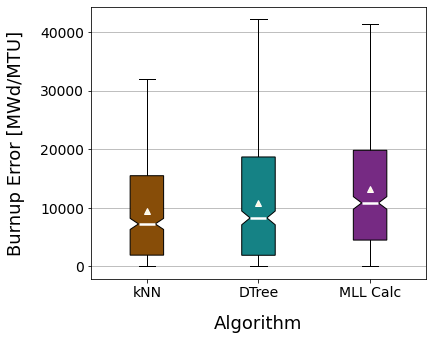
\includegraphics[width=\textwidth]{./chapters/exp1/sfcompo_boxplots_impnull_burn.png}
    \caption{Box plots of burnup errors using mean-imputed null values.}
    \label{fig:burnimp}
  \end{subfigure}
  \hfill
  \begin{subfigure}[b]{0.49\textwidth}
    \centering
    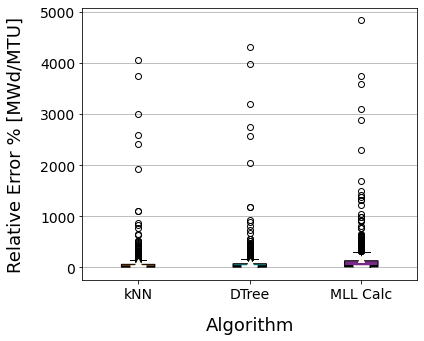
\includegraphics[width=\textwidth]{./chapters/exp1/sfcompo_boxplots_impnull_pcterr_burn.png}
    \caption{Box plots of burnup percentage errors using mean-imputed null values.}
    \label{fig:burnimppct}
  \end{subfigure}
  \vskip\baselineskip
  \begin{subfigure}[b]{0.49\textwidth}
    \centering
    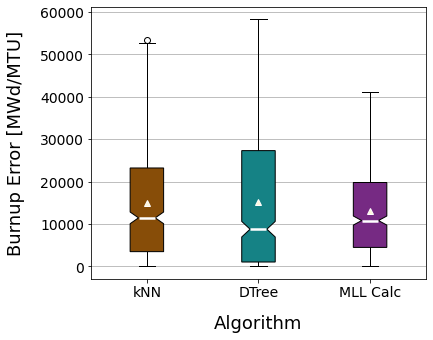
\includegraphics[width=\textwidth]{./chapters/exp1/sfcompo_boxplots_0null_burn.png}
    \caption{Box plots of burnup errors using zero-replaced null values.}
    \label{fig:burn0}
  \end{subfigure}
  \hfill
  \begin{subfigure}[b]{0.49\textwidth}
    \centering
    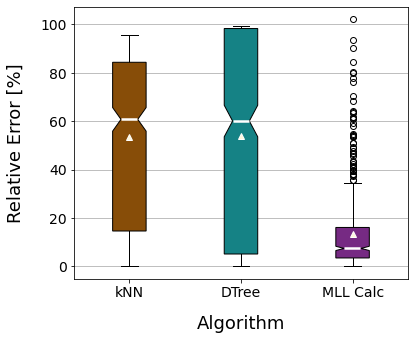
\includegraphics[width=\textwidth]{./chapters/exp1/sfcompo_boxplots_0null_pcterr_burn.png}
    \caption{Box plots of burnup percentage errors using zero-replaced null values.}
    \label{fig:burn0pct}
  \end{subfigure}
  \caption{Box plots of burnup prediction errors and percentage errors for each 
           algorithm using two missing entry techniques: imputation with mean 
           values and replacement with zero.}
  \label{fig:sfcoburn}
\end{figure}

The ranges seen for the imputed nulls test set in Figure \ref{fig:burnimppct}
are as large as they are from low burnups ($< 10 GWd/MTU$) being far
overpredicted, since a small number in the denominator will yield a high
percentage error. A large subset of the low burnup cases are \gls{PHWR}s.
Their burnups are also unlikely to be predicted well because of the inability
of \gls{PHWR} reactors to be represented accurately with this methodology.
Removing the \gls{PHWR} reactors from the results removes all outliers with
percentage errors larger than 1750\%. That is still a very high relative error,
but there are other low burnup cases in the database.  Removing \gls{PHWR}s
does not significantly alter the zero-nulls results in Figure
\ref{fig:burn0pct}.

The range of percentage errors for the zero-nulls test set in Figure
\ref{fig:burn0pct} tells a different story. There is only one case (an
\gls{MLL} outlier) that is above 100\% error.  While the absolute errors for
the scikit-learn algorithms in Figure \ref{fig:burn0} span a larger range than
their counterparts in Figure \ref{fig:burnimp}, their relative errors remain
within $0-100\%$. The only case that predicts the burnup well is the \gls{MLL}
method with the zero-null missing values treatment of the \gls{SFCOMPO} test
set, but about 8\% of the test cases are outliers.  If the best-case median
error of $1.7 GWd/MTU$ in Table \ref{tbl:sfcoburn} were to also correspond to a
lower relative error, then that would be an acceptable result.  However, while
the \gls{MLL} calculations have a percentage error below 20\% at the 75\%
quartile, the non-outlier data reaches almost 40\% and the 8\% of the data
reaches 100\%.

Overall, the absolute errors in Table \ref{tbl:sfcoburn} tell a much more
encouraging story than the box plots in Figure \ref{fig:sfcoburn}, so
investigating beyond the mean and median absolute errors was necessary to show
the real picture of this unique testing scenario. 

\noindent \textbf{\gls{U235} Enrichment}

For both reactor type classification and burnup regressoion, the zero-nulls
test set predicted by \gls{MLL} calculations far outperform all other
algorithm/test set scenarios. However, the enrichment regression results break
this trend.  Table \ref{fig:sfcoenri} shows that decision trees outperform the
other methods, and furthermore, there isn't a large difference in performance
between the two test sets, expecially seeing that the median absolute error is
the same for both test sets.  The other two algorithms follow their previous
behavior: moving from imputed nulls to zero-nulls, \textit{k}-nearest neighbors
has worse performance and \gls{MLL} calculations has better performance.

\begin{table}[!htb]
  \centering
  \begin{tabular}{@{}m{1.5in}llllll@{}}
    \toprule
                     & \multicolumn{3}{m{2in}}{Mean Errors [\% U235]} & \multicolumn{3}{l}{Median Errors [\% U235]} \\ \toprule
    Null Handling    & kNN           & DTree          & MLL          & kNN            & DTree          & MLL    \\ \midrule
    Imputed Nulls    & 0.72          & 0.31           & 1.25         & 0.50           & 0.22           & 1.13   \\
    Zero-value Nulls & 1.67          & 0.36           & 0.49         & 2.02           & 0.22           & 0.35   \\ \bottomrule
  \end{tabular}
  \caption{Mean and median errors for enrichment prediction of the \gls{SFCOMPO} 
           test cases.}
  \label{tbl:sfcoenri}
\end{table}

The mean and median absolute errors are also visible with more statistical
information in the box plots in Figure \ref{fig:sfcoenri}. The outliers for
decision trees and \gls{MLL} calculations are 30 and 16 for the imputed nulls
in Figure \ref{fig:enriimp}, respectively. So although decision trees provides
a typically low absolute error, the outliers reach nearly as far as the spread
of \textit{k}-nearest neighbors. The number of outliers for the zero-nulls
results in Figure \ref{fig:enri0} are 45 and 16 for decision trees and
\gls{MLL} calculations, respectively.  The spread of the outliers for these
algorithms is similar to the previous figure, but \textit{k}-nearest neighbors
has a larger spread of absolute error.

\begin{figure}[!htb]
  \centering
  \begin{subfigure}[b]{0.49\textwidth}
    \centering
    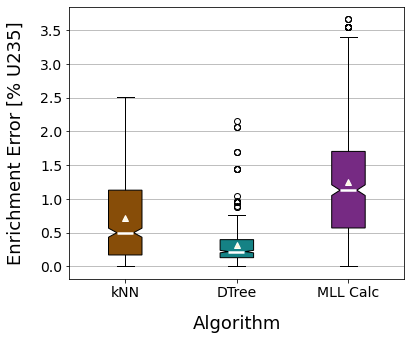
\includegraphics[width=\textwidth]{./chapters/exp1/sfcompo_boxplots_impnull_enri.png}
    \caption{Box plots of enrichment errors using mean-imputed null values.}
    \label{fig:enriimp}
  \end{subfigure}
  \hfill
  \begin{subfigure}[b]{0.49\textwidth}
    \centering
    \includegraphics[width=\textwidth]{./chapters/exp1/sfcompo_boxplots_impnull_pcterr_enri.png}
    \caption{Box plots of enrichment percentage errors using mean-imputed null values.}
    \label{fig:enriimppct}
  \end{subfigure}
  \vskip\baselineskip
  \begin{subfigure}[b]{0.49\textwidth}
    \centering
    \includegraphics[width=\textwidth]{./chapters/exp1/sfcompo_boxplots_0null_enri.png}
    \caption{Box plots of enrichment errors using zero-replaced null values.}
    \label{fig:enri0}
  \end{subfigure}
  \hfill
  \begin{subfigure}[b]{0.49\textwidth}
    \centering
    \includegraphics[width=\textwidth]{./chapters/exp1/sfcompo_boxplots_0null_pcterr_enri.png}
    \caption{Box plots of enrichment percentage errors using zero-replaced null values.}
    \label{fig:enri0pct}
  \end{subfigure}
  \caption{Box plots of enrichment prediction errors and percentage errors for 
           each algorithm using two missing entry techniques: imputation with 
           mean values and replacement with zero.}
  \label{fig:sfcoenri}
\end{figure}

Again, a look at the relative errors gives a different sense of these results.
Figures \ref{fig:enriimppct} and \ref{fig:enri0pct} present the percent error
statistics for the imputed nulls and zero-nulls test sets, respectively.  In
Figure \ref{fig:enriimppct} there are 57, 39, and 49 outliers for the
\textit{k}-nearest neighbors, decision trees, and \gls{MLL} calculations,
respectively.  In Figure \ref{fig:enri0pct} there are 44 and 23 outliers for
the decision trees and \gls{MLL} calculations, respectively.

As with the burnup regression, the high percentage errors are caused by a large
overprediction of enrichments that are of low value. All of the \gls{PHWR}s fit
into this category, and removing them from the results removes the outliers
with the highest errors from the imputed nulls results in Figure
\ref{fig:enriimppct}, leaving a maximum of 250\% enrichment error. This is
still a high maximum error because there are other low enrichments not
belonging to the \gls{PHWR} class that remain overpredicted.  As with the
burnup, removing \gls{PHWR}s does not significantly alter the zero-nulls
results in Figure \ref{fig:enri0pct}.

Unlike the case with burnup, the decision trees algorithm gives a better
performance that is null handling-independent than the other algorithm/test set
scenarios. Although there was a slightly worse mean absolute error for the
zero-nulls test set (the median absolute error was the same), the relative
error remains below 100\% for all outliers, as seen in Figure
\ref{fig:enri0pct}.  This makes the decision trees algorithm with the
zero-nulls test set the best performing case for enrichment regression.

It is again true that investigating relative error statistics alongside
absolute error statistics provides a fuller picture of the regression of the
\gls{SFCOMPO} database entries.  It is an unexpected result to have either one
of the scikit algorithms outperform \gls{MLL} calculations for the zero-nulls
test set, since they tended to have lower errors using the imputed nulls test
set. 




\section{Summary}

This chapter covers the details of the methodology in four main sections:
training set simulations, information reduction, statistical methods
implementation, and performance evaluation. This approach focuses on the
situation where there is a full set of well-measured nuclides, some of which
require destructive techniques to measure, which will later be contrasted to a
set of nuclides that are measured in a non-destructive manner. 

First, in Section \ref{sec:training1}, the training data is simulated, which
provides an array of nuclide measurements as the features. The prediction
parameters are the simulation inputs: reactor type, burnup, \gls{U235}
enrichment, and time since irradiation.  The reactor types are one of three
common commercial reactors: \gls{PWR}, \gls{BWR}, or \gls{PHWR}.  The burnup is
measured in $MWd/MTU$ and ranges from 0 to about $68,000$ in 21-28 timesteps
depending on the reactor type.  The enrichment is $\%U235$ and is centered
around the following percentages: 0.5, 1.5, 2.0, 3.0, 4.0, 5.0, and 0.711
(natural \gls{U235} enrichment for the \gls{PHWR}s).  The time since
irradiation is measured in $days$ and ranges from 0 to 6000, or 16 years, in
$100-day$ time steps with 61 total steps. Given these simulation inputs, the
makeup of 4.5e5 \gls{SNF} entries are simulated using \gls{ORIGEN} \cite{scale,
origen, origenarp}.

Second, in Section \ref{sec:inforeduc1}, information reduction on the training
set is carried out using randomly injected uniform error. The random error is
used to study the robustness of the methodology to artificial noise in the
feature set, which is comprised of 29 nuclide masses.  The introduced training
set error is increased up to 20\%.

Third, in Section \ref{sec:statmodel1}, three algorithms, \textit{k}-nearest
neighbors, decision trees, and \gls{MLL} calculations, are used to train models
to predict the four reactor parameters of interest.  The first two are
algorithms implemented using the scikit-learn python \gls{ML} toolkit, and
\gls{MLL} is implemented in python leveraging SciPy and NumPy for fast
likelihood calculations \cite{scikit, scipy, numpy}.  For the scikit
algorithms, the hyperparameters governing model complexity were optimized to
minimize the prediction errors.  The scripts written to run the scikit-learn
predictions and the \gls{MLL} calculations were deployed using
\gls{UW}--Madison's \gls{CHTC} resources, the \gls{UW} campus grid, and the
\gls{OSG} \cite{osg07, osg09}.  

Fourth, in Section \ref{sec:eval1}, the prediction errors are evaluated to draw
conclusions about the capability of the chosen statistical methods to inform
\gls{SNF} attribution with increasingly less precise material measurements.
Sections \ref{sec:randerrA} and \ref{sec:randerrB} show the results of
information reduction by injecting noise into the training set (randomly
applied uniform error).  Next, the impacts of training set size are evaluated
to understand the effects of model generalization in Section
\ref{sec:randerrC}. After this, the impacts of having prior knowledge of the
reactor type on the quality of prediction of the regression cases are studied
in Section \ref{sec:randerrD}. Last, the external testing set, the
\gls{SFCOMPO} database, is used to test this methodology in Section
\ref{sec:sfcompo}. 

For Sections \ref{sec:randerrA}--\ref{sec:randerrD}, the prediction performance
is measured by using the training set to provide testing samples. The entire
training set is tested at some point; when a test sample is used, it is first
removed from the training set so that there is no exact replica of it in the
training stage. For the scikit-learn algorithms, this is accomplished via
5-fold \gls{CV}, and the \gls{MLL} calculations test one training set entry at
a time.  Impacts of increasing training set error on the four prediction
parameters are covered in Sections \ref{sec:randerrA} and \ref{sec:randerrB}
The \gls{MLL} calculations method is the most resilient to introduced error,
followed by decision trees then \textit{k}-nearest neighbors. The behaviors of
each algorithm's performance degradation for reactor type, burnup, and
enrichment all behave in a similar fashion. But the \textit{k}-nearest
neighbors prediction of time since irradiation has a drastic drop that
starts with even 1\% introduced training set error. The prediction performance
at 20\% training set error is used as a baseline for future work. 

In Section \ref{sec:randerrC}, the impacts of fewer training set entries are
implemented to investigate how the algorithms each generalize to unseen samples. Using the
training set that has 5\% error, it was reduced in four steps from its full
size, the lowest size being 20\% of the full training set. Although the
\gls{MLL} calculations perform above the scikit-learn algorithms at most sizes,
the data points at 20\% training set size show \gls{MLL} below one or both of
the scikit-learn algorithms. The takeaway is that while this training set is
more than large enough to achieve good performance from a high variance
approach, the performance may not hold with a different training set design. 

Section \ref{sec:randerrD} shows whether the burnup, enrichment, and time since
irradiation predictions benefit from having the prior knowledge of reactor
type.  The largest improvement is for the \gls{PHWR} (only 1.5\% of training
set) regression cases for the scikit-learn algorithms, whereas there is no
improvement for \gls{MLL} calculations. Because the \gls{BWR} class dominates
the training set, there is modest improvement in \gls{PWR} regression cases as
well for the scikit-learn algorithms.

Last in this chapter is Section \ref{sec:sfcompo}, where the performance of
this methodology using real world test cases of nuclide concentration
measurements via the \gls{SFCOMPO} database is demonstrated.  While the
training set design spans the label space that exists in \gls{SFCOMPO}, there
are many missing measurements from the features in the training set, which is
comprised of 29 nuclide masses.  Because of an imbalanced training set and the
method used to handle the null values, the reactor type classification results
are poor, which translates to the regression cases as well.  The \gls{MLL}
calculations perform the best, but many of the prediction errors are still
large. It is possible that because most of the 505 entries contain many of the
of-interest uranium and plutonium isotopes, that this testing set should be
used only in a study limited to those isotopes. They are known to provide good
discrimination on their own \cite{pu_discrimination, nicolaou_2006,
nicolaou_pu, nicolaou_2009, nicolaou_2014, nicolaou_2015}.


\begin{frame}
  \frametitle{Statistical Learning with Gamma Spectra}
  \textbf{Goals} : Understand limits of real-world scenario
  \begin{enumerate}
    \item Level of reduction in reactor parameter prediction
    \item Best performing methods
  \end{enumerate}

  \textbf{Variables}
  \begin{enumerate}
    \item the complexity of the ML algorithm used, 
    \item feature reduction (implicit), and 
    \item quality of training and/or testing data set.
  \end{enumerate}
\end{frame}

\begin{frame}
  \frametitle{Statistical Learning with Gamma Spectra}
  \textbf{Qualitative Hypotheses}
  \begin{itemize}
    \item Complex algorithm will provide best behavior
    \item Indirect isotopics $=$ implicit feature reduction: less accurate
    \item Higher quality gamma spectra will yield better results
  \end{itemize}

  \textbf{Risk Mitigation}
  \begin{itemize}
    \item New algorithms: tree-based, neural nets, Bayesian MLE
    \item Further manual or statistical preprocessing
    \item Add isotope identification step
  \end{itemize}
\end{frame}


\chapter{Conclusions and Future Work}
\label{ch:concl}

This chapter focuses on concluding remarks and future work.  First, a summary
is outlined in Section \ref{sec:summary}, Next, in Section \ref{sec:concl}, the
main experimental results from each section are brought together to discuss the
bigger picture of this work.  Additionally, there are areas of the methodology
that are simplified and several avenues this work could pursue, so this is
discussed in Section \ref{sec:future}.

\section{Summary}
\label{sec:summary}

The main research question that this work addresses is as follows: \textit{How
does the ability to determine forensic-relevant spent nuclear fuel attributes
using machine-learning techniques degrade as less information is available?}. 
The workflow to examine this question takes place in four steps.  

First, the training data is simulated, which provides an array of nuclide
measurements as the features. The prediction parameters are the simulation
inputs: reactor type, burnup, \gls{U235} enrichment, and time since
irradiation.  The reactor types are one of three common commercial reactors:
\gls{PWR}, \gls{BWR}, or \gls{PHWR}.  The burnup is measured in $MWd/MTU$ , the
enrichment is measured in $\%{}^{235}\text{U}$, and the time since irradiation
is measured in $days$. The size of the training set is $4.5 \times 10^5$
\gls{SNF} entries, which were simulated using \gls{ORIGEN} \cite{scale, origen,
origenarp}.  These steps are covered in Sections \ref{sec:training1} and
\ref{sec:training2}.

Second, information reduction on the training set is carried out using randomly
injected uniform error or computationally generated gamma spectra. For the
former, the training set is comprised of nuclide masses and the random error is
used to study the robustness of the methodology to artificial noise in the
feature set.  For the latter, the training set becomes lists of summed energy
windows of the gamma spectra, which were computed from nuclide activity
measurements using \gls{GADRAS} \gls{DRF}s for six detectors \cite{gadras}.
Each detector-based training set undergoes three different methods of
processing the gamma spectra, denoted as auto, short, and long energy windows
lists.  These steps are covered in Sections \ref{sec:inforeduc1} and
\ref{sec:inforeduc2}.

Third, three algorithms are used to predict the four reactor operation
parameters in this work: \textit{k}-nearest neighbors, decision trees, from the
scikit-learn python \gls{ML} toolkit, and \gls{MLL} calculations, implemented
in python using SciPy and NumPy \cite{scikit, scipy, numpy}.  For the scikit
algorithms, the hyperparameters governing model complexity were optimized to
minimize the prediction errors.  All of the code was run using
\gls{UW}--Madison's \gls{CHTC} resources, the \gls{UW} campus grid, and the
\gls{OSG} \cite{osg07, osg09}.  These steps are covered in Sections
\ref{sec:statmodel1} and \ref{sec:statmodel2}.

Fourth, the prediction errors are evaluated to understand the increase in error
as the information supplied is less precise. This impacts the conclusions that
can be formed about the capability of simple statistical methods to inform
nuclear material attribution.  The testing samples come directly from the
training set, and the prediction errors from  these testing sample are what is
studied for the performance.  When a test sample is used, it is first removed
from the training set so that there is no exact replica of it in the training
stage.  This testing scheme allows the entire training set to be tested
eventually.  It is accomplished via 5-fold \gls{CV} for the scikit-learn
algorithms and by testing one training set entry at a time for the \gls{MLL}
calculations.  These results are presented in Sections \ref{sec:eval1} and
\ref{sec:eval2}, and are summarized as follows.

\section{Conclusions}
\label{sec:concl}

\noindent \textbf{Reactor Parameter Prediction Using Nuclide Masses}

%This experiment is a demonstration of the methodology with the
%"perfect knowledge" of nuclide masses. Information reduction is accomplished by
%adding noise to the training set in the form of randomly applied uniform error.
%The results are in Sections \ref{sec:randerrA} and \ref{sec:randerrB}.  In
%order to understand the ability of the models to generalize, the performance
%with respect to training set size is studied in Section \ref{sec:randerrC}.
%Section \ref{sec:randerrD} introduces the impacts of having prior knowledge of
%the reactor type on the quality of prediction of the regression cases.  Last,
%the external testing set, the \gls{SFCOMPO} database, is used to test this
%methodology against sometimes complicated real world data sets in Section
%\ref{sec:sfcompo}. 

Sections \ref{sec:randerrA} and \ref{sec:randerrB} demonstrate the impacts of
injected training set noise on the prediction parameters. Aside from the
\textit{k}-nearest neighbors prediction of time since irradiation, all of the
algorithms follow a similar pattern for each prediction scenario.  The
\gls{MLL} calculations are the most resilient to introduced error, followed by
decision trees then \textit{k}-nearest neighbors.  \textit{It is difficult to
state whether or not these results are "good enough" on their own, but they do
serve as a useful baseline for the results in Chapter \ref{ch:exp2}.} 

Next, the model generalization is studied in Section \ref{sec:randerrC} by
creating learning curves using $20-100\%$ of the training set.  It shows that
the training set is large enough for the \gls{MLL} calculations to remain the
best performing method until the 20\% training set size, when those data points
dip below one or both of the scikit-learn algorithms depending on the
prediction parameter.  \textit{This performance is highly dependent on the
training set design because these are qualitatively high variance methods
(compared to common algorithms not shown in this work) that do not generalize
well.}

Section \ref{sec:randerrD} investigates the effect of having reactor type prior
knowledge on burnup, enrichment, and time since irradiation prediction.  There
is modest and significant improvement for \gls{PWR} and \gls{PHWR} cases,
respectively, since they are both the minority classes in the training set.
These improvements only exist for the scikit-learn algorithms, since the
\gls{MLL} calculations are not affected by reactor type knowledge. \textit{The
key takeaway is that regression cases linked to \glspl{PHWR}s are not expected
to perform well.}

The last study in this chapter is in Section \ref{sec:sfcompo}, where an
external test set is used that is comprised of measurements from real
commercial power \gls{SNF} from around the world: the \gls{SFCOMPO} database.
The main challenge with this database are that many entries only contain
measurements for uranium and plutonium isotopes, and the missing measurements
are inconsistent. Two methods were implemented: imputing the null values with
the mean of a given feature, and imputing the null values with zero.  The
reactor type classification results are very poor except for the \gls{MLL}
predictions using zero-valued nulls.  This combination also best predicts the
burnup, but oddly, the decision trees for both methods of null handling best
predicts the enrichment.  \textit{Overall, the errors are still quite large, so
the \gls{SFCOMPO} database presents challenges to being used with this
methodology. The techniques for improving the performance are discussed next in
the future work suggestions, Section \ref{sec:future}.}

\noindent \textbf{Reactor Parameter Prediction Using Processed Gamma Spectra}

%This experiment's purpose is to probe the
%usefulness of field-deployable detectors for giving rapid information about
%presumed \gls{SNF}. The information reduction is achieved by using
%computational gamma spectra of various detectors with decreasing detector
%energy resolution.  The gamma spectra of each \gls{SNF} entry are processed in
%three different manners, resulting in three energy windows lists, denoted by
%auto, short, and long.  

The reactor type classification results are first covered in Section
\ref{sec:exp2_rxtr}.  Unsurprisingly, the \gls{MLL} calculations consistently
perform the best across the algorithms. There is a slightly better overall
performance by the short energy windows list as compared to the others,
although the large variation by the auto energy windows lists has some data
points performing better.  The confusion matrices show the details of every
data point, but most of the misclassifications are \gls{PWR} and \gls{PHWR}
being labeled as \gls{BWR}.  The only algorithm-detector combinations that
exceed the baseline are the \gls{MLL} calculations for the lab-based \gls{HPGe}
with all three energy windows lists and the \gls{MLL} calculations for the
\gls{SrI2} detector with the auto energy windows list. \textit{Given the choice
in baseline, reactor type classification is only acceptable for the four cases
exceeding it and the three full-knowledge training sets.}

Next, the regression cases are shown in Section \ref{sec:exp2_reg}.  Regardless
of the energy windows list, the detector-based training sets all do the
following for the \gls{MAPE} and \gls{MAE}: the burnup tends to far outperform
the baseline, the enrichment consistently underperforms with respect to the
baseline, and the time since irradiation has values along the baseline, where
many are below line but close to it.  The spread of absolute errors including
the outliers shows that there is a significant portion of the training set that
is being predicted with very large errors; the spread of outliers encompassed
$3-17\%$ of the training set depending on the case.  Studying these results
with respect to the \gls{MedAE}, the burnup and time since irradiation
predictions do well with respect to their baselines.  \textit{Relative to the
baseline, the burnup prediction performs well over an acceptable level,
enrichment prediction performs well under an acceptable level, and time since
irradiation prediction has several cases that perform at or near the acceptable
level.} Additionally, there is not a large difference in performance among the
three energy windows lists.  \textit{This suggests that the performance is
indepedent of the gamma spectra processing approaches.} 

\noindent \textbf{Post-Conclusions Discussion}

Despite many of the nuclides that are included in the short and long energy
windows lists having known poor simulation quality \cite{pwr_benchmark_2010,
skutnik_2021}, the burnup prediction clearly had enough information to do well.
The poor enrichment prediction is likely because the detected radionuclides are
not enrichment indicators, although ${}^{152}\textit{Eu}$ is and should be
included in the long energy windows list.\todo{152Eu was in top feature impt
list} The time steps in the training set being about $100\:days$ was a limiting
factor in its quality of prediction; many of the \gls{MAE} values were around
this level in the second experiment. 

There is a clear leader throughout all of the results in terms of being a
consistent best performer: the \gls{MLL} calculations. The reason it can
perform well, though, is because of the large number of simulations.  If there
were to be a training set of much higher fidelity but larger steps between the
training set labels, it is possible \gls{MLL} would not be a top performer. 

The two scikit-learn algorithms still had some interesting variation in their
prediction capabilities despite usually under-performing. Decision trees best
predicted the enrichment for the external testing set scenario with
\gls{SFCOMPO}. For all of the 0\% training set error cases in the first
experiment, the scikit-learn algorithms performed better.  The \gls{MLL}
robustness to error is likely from the different manners in which the error was
applied.  The scikit-learn approach was to change the training set feature
itself to a new value within some range based on the error, but the \gls{MLL}
approach was to include this error instead as uncertainty. In this way, it is
not affecting the features directly, just the resulting uncertainty of the
log-likelihood calculation. If the same approach was used, or some error
existed in the measurements, \gls{MLL} again might not be the best choice. 

Another way in which the implementation differed was the 5-fold \gls{CV} being
used as the testing protocol for the scikit-learn algorithms. For 5 rounds,
20\% of the training set is removed as a testing set, where eventually all 5
folds are tested.  By contrast, the \gls{MLL} test samples get removed a single
entry at a time.  If the training set were to be more sparsely populated with
the same range of each label, this would be of larger concern.  From the
learning curves in Figure \ref{fig:learns}, it appears that reducing the
training set by 20\% would in theory not impact the \gls{MLL} performance, but
it is still a major difference in implementation. 

It should be noted that the injection of error in the training set in the same
manner as the test samples is not necessarily realistic. In a real-world
scenario, the training database would be quite accurate and the testing samples
might have variable error. 

The nuclide-based feature sets (i.e., 29 nuclide masses and 32 nuclide
activities) in both experiments were determined by external factors, i.e., the
\gls{SFCOMPO} database measurements and the radionuclides available in
\gls{GADRAS}.  Since each training set is designed to be able to predict all
four labels, not all features are relevant to a given label. This could add
noise for a given label prediction if there are only a handful of relevant
features. 

With respect to the number of features affecting the prediction performance for
the detector-based training sets, the overall similarity of performance among
the three energy windows lists might mean that the feature numbers are not
impacting the algorithms much.  Another explanation is that they all include
too many features (outside of the scintillator detectors with the auto energy
windows list).  It is possible that even the short list with 42 features has
too high of a dimension for these methods to perform well. The statement from
above also applies, that if only a few features are relevant, the remaining
ones only add noise. 

The automatic peak searching approach results in erratic behavior for the
scikit-learn algorithms. Noting the poor performance of the high energy
resolution detectors, this is presumably from the added noise of including all
peaks instead of just targeted peaks like the other two lists.  It is still a
promising approach for the lower energy resolution detectors, and possibly even
the high energy resolution detectors since in theory one could filter the noise
from the detector peak searches. 

\section{Future Work}
\label{sec:future}

When designing any study, simplifications and assumptions must be made to take
a first-order look at the problem. Additionally, any good exploration is likely
to generate more questions than answers. This final section covers a list of
future work based on the the simplifications made and questions created.

\subsection{Training Set Features}

\noindent \textbf{Simulation Fidelity}

\gls{ORIGEN-ARP} not only offers computational expediency, but the training set
creation was able to be fully scripted and automatically carried out. The $4.5
\times 10^5$ entries in the training set were simulated in a matter of hours on
a personal computer.  

Section \ref{sec:fidelity} discusses the fidelity of the simulations used to
create the training database, and how the ground truth in this work is
therefore not perfect truth.  The first improvement to be made with the
training set is filtering out problematic-to-simulate nuclides, such as
${}{125}\text{Sb}$. An exercise was carried out to compare \gls{ORIGEN-ARP}
simulations to an entry in \gls{SFCOMPO}, and there were some nuclide
discrepancies that reached 40\%. It would be better to remove these from
consideration if they are systematically poorly simulated.

One level beyond this would be to forego the convenience that \gls{ORIGEN-ARP}
provides and use higher fidelity simulations in \gls{SCALE}.  Maximizing the
accuracy of the training set is worthwhile, since it is a static entity that is
only simulated once. 

\noindent \textbf{Feature Set Study}

The lists of training set features in this work were not chosen based on
knowledge of nuclear reactor operation and the best signatures for the various
labels being predicted (reactor type, burnup, ${}^{235}\text{U}$ enrichment,
time since irradiation).  Instead, they were chosen based on the nuclide
availability in the \gls{SFCOMPO} database and the computational gamma spectra
tool, \gls{GADRAS}, which gave 29 and 32 nuclides, respectively. 

For the 29 nuclide mass training set, a small feature importance exercise was
carried out to determine if these lists could be reduced further. This was
carried out by using \texttt{SelectKBest(score\_func=f\_regression,
k=29).fit(X,y)} (or \texttt{f\_classif} for reactor type classification),
sorting the scores of the features, choosing the top $N$ features for each
label, and taking the set of features together for all labels.  The resulting
set of best-scoring features for all the labels included most or all of the
original list depending on the arbitrary decision of $N$.  This could be
further refined by combining domain knowledge of reactor physics and a more
structured statistical feature importance approach. Furthermore, because mass
spectrometry provides ratios of nuclides, studying how various ratios perform
versus nuclide masses or nuclide concentrations with respect to initial uranium
mass would be prudent. 

\noindent \textbf{Gamma Spectra Processing}

For the 32 nuclide activity training set, the most detectable gamma energies
emerged from the short and long energy windows lists to include from 7 and 12
nuclides, respectively, shown in Table \ref{tbl:enlistnucs}. So in this way,
nuclear physics performed the feature selection.  It is clear from the results
that the 7- and 12-nuclide lists performed quite well, and exceeded the
baseline for all four prediction scenarios.  However, there were many high
energy photopeaks excluded from these lists that might provide more
information. These were captured via the auto peak search method, but the
resulting energy windows list did not provide better results (and in some cases
with \textit{k}-nearest neighbors, provided worse performance).  This simple
approach should be refined with a study on the latest gamma spectra processing
tools and which are suitable to process a training set of $4.5 \times 10^5$
spectra within a reasonable amount of time. 

There are also more advanced detection techniques being studied, some which
could be simulated with \gls{GADRAS}.  This would provide easier peak
processing for nuclides of interest, e.g., with peaks at the high energy end of
the spectrum.

Citations:

targeted or advanced measurement techniques \cite{snf_gamma, compton_supp,
bwr_high-res_gamma, pwr_bwr_gamma}

innovative spectra evaluation and radioisotope identification methods
\cite{riid_09, rapid_riid_18, sull_gen_07, sull_valid_15, sull_auto_17,
sull_unc_17}.

\todo{finish and update citations}

\subsection{Statistical Method Optimization}

The methods in this work all have high variance, and so it would have seemed
prudent to apply stronger regularization. However, hyperparameter optimization
did not shift the high variance defaults much towards more bias.  The resulting
inability to generalize likely was a contributing factor to the large errors in
the results when using the \gls{SFCOMPO} database as a testing set. A closer
look at optimization is warranted in tandem with the above work on the feature
sets for each label.

Since the \gls{MLL} approach is essentially \textit{k}-nearest neighbors with
$k=1$ and a different loss metric, the \gls{MLL} calculations could be expanded
to include the option to have \textit{k} samples averaged for a response, which
would increase the bias.  Another option would be to use the likelihood
calculations as custom sample weights within the \textit{k}-nearest neighbors
algorithm. The implementation of \textit{k}-nearest neighbors in this work used
Manhattan distance $d_i$ with samples weighted by $1/d_i$. This would change
the sample weights to $L(M|x_{test})$, the likelihood as calculated in Equation
\ref{eq:like}.

It is entirely possible that optimizing the methods in this work can only
improve the prediction performance by a minimal amount, and that more complex
methods could be beneficial. Because of this possibility, a broader survey of
statistical methods with this training set is another possible next step. 

\subsection{Serial Prediction}

Figure \ref{fig:knownrxtr} shows that for some combinations of prediction label
and algorithm, there is an improvement in the regression performance for the
\gls{PHWR} class, and less so for some \gls{PWR} cases.  (There was no
significant improvement seen for any reactor type/regression case combination
for the \gls{MLL} calculations.) Given the majority of the database is
comprised of \gls{BWR} entries, the improvement is not surprising; it is the
lack of improvement in the other cases that is unexpected. Either way, it makes
sense to first determine the reactor type before performing the other
predictions if not using the \gls{MLL} approach. One example of this being
done is in Reference \cite{serial_ml}.

Performing regression after first classifying the reactor type means much care
should be taken to have a robust reactor type classification algorithm. One way
to ensure better classification is by implementing a study that leverages
\gls{ROC} curves. \Gls{ROC} curves plot the true positive rate (vertical axis,
$\frac{\text{True Positives}}{\text{True Positives + False Negatives}}$) with
respect to the false positive rate (horizontal axis, $\frac{\text{False
Positives}}{\text{False Positives + True Negatives}}$) for various
\textit{decision thresholds}, as shown in Figure \ref{fig:roc} \cite{roc}.

\begin{figure}[!htb]
  \centering
  \includegraphics[width=0.8\linewidth]{./chapters/concl/roc.png}
  \caption[Example of an \acrshort{ROC} curve]
          {Example of an \acrshort{ROC} curve showing the decision threshold 
           (probability of class belonging) changing from $\infty$ to 0.1; this 
           is borrowed from Reference \cite{roc}.}
  \label{fig:roc}
\end{figure}

During prediction of a test sample, the scikit-learn classifiers calculate a
probability that the sample belongs to a given class. In binary prediction, the
default threshold is 0.5. A probability above this threshold means the sample
will be predicted to belong to the positive class, and below that the sample
will belong to the negative class.  In multi-class prediction, the highest
probability is chosen as the predicted class.

An ideal classifier would have values along the vertical axis and then straight
across the top, meaning beyond some threshold value there are zero false
positives. On the other end of the spectrum, if the classifier being used in
Figure \ref{fig:roc} were only choosing classes randomly, it would follow an
$x=y$ diagonal line. The one shown here performs somewhere in between these two
extremes. 

If the algorithm returns the probabilities of class belonging instead of the
predicted class, the threshold can be tuned after the fact to complete
predictions.  With this work, e.g., the decision threshold  could be manually
tuned to require a higher threshold for \gls{BWR} classification. If that were
the case, there could be fewer misclassifications of \glspl{PHWR}s and
\glspl{PWR}s as \glspl{BWR}s. The issues with regression of \glspl{PHWR}s could
then be resolved if they were accurately classified as such beforehand. T

\subsection{SFCOMPO}

The \gls{SFCOMPO} database being used as an external test set within the
framework of this methodology performed poorly in the sense that some relative
errors were extremely large.  Section \ref{sec:sfcompo} shows the results using
two different methods for handling the missing measurement values: imputation
with the mean value of a given nuclide, and replacing the null values with
zero. 

One way to improve the results is using the previously discussed serial
prediction approach, where the reactor type is first determined before the
regression cases are predicted using training sets that only include entries
from the predicted reactor type.  This was partially touched on in Section
\ref{sec:sfcompo} by discussing the largest relative errors disappearing when
\glspl{PHWR}s were removed from consideration.  Another way that might improve
the results is with better simulation fidelity, also previously discussed. 

A third approach is revisiting the method by which the missing measurements are
handled.  One option is to side-step the missing nuclide measurements all
together.  Reducing the training set to only consider uranium and plutonium
isotopes accomplishes this; the majority of measurements in the training set
would exist and there would be very few missing measurements.  This is
essentially what the zero-valued nulls with \gls{MLL} calculations does, and
likely why it performed the best for the reactor type and burnup predictions
(and a close second for the ${}^{235}\text{U}$ enrichment prediction). 

Although the zero-null values approach is likely to always perform the best
with \gls{MLL} calculations, there are better approaches than mean (or median)
null value imputation. For example, one could take a \textit{k}-nearest
neighbors approach to imputation where the mean, median, or mode of the
\textit{k}-closest samples are used for imputation (rather than the mean,
median, or mode of the entire column in that testing set). Another approach for
handling missing values is outlined in Reference \cite{nf_missingdata}, where a
novel imputation approach for the \gls{SFCOMPO} database, called Monte Carlo
Bayesian Database Generation, is discussed.



%% Do you have appendices?  If so, add them here, just like chapters.
% \begin{appendices}
% \include{backmatter/appendix1}
% \end{appendices}

%% McBride is a very nice style (some version is included in this distribution)
\bibliographystyle{mcbride}
\bibliography{dissertation}

\end{document}
